%% Apêndices

\begin{apendicesenv}

\partapendices

\chapter{Telas da Aplicação -- Creator Workbench}

Este apêndice apresenta as principais telas do Creator Workbench na versão final, agrupadas pelas partes do sistema.

\section{Acesso e cadastro}

\begin{figure}[H]
    \centering
    \caption{Tela de \textit{login}, com acesso por e-mail e senha e atalhos para recuperar a senha e solicitar cadastro}
    \label{fig:tela-01}
    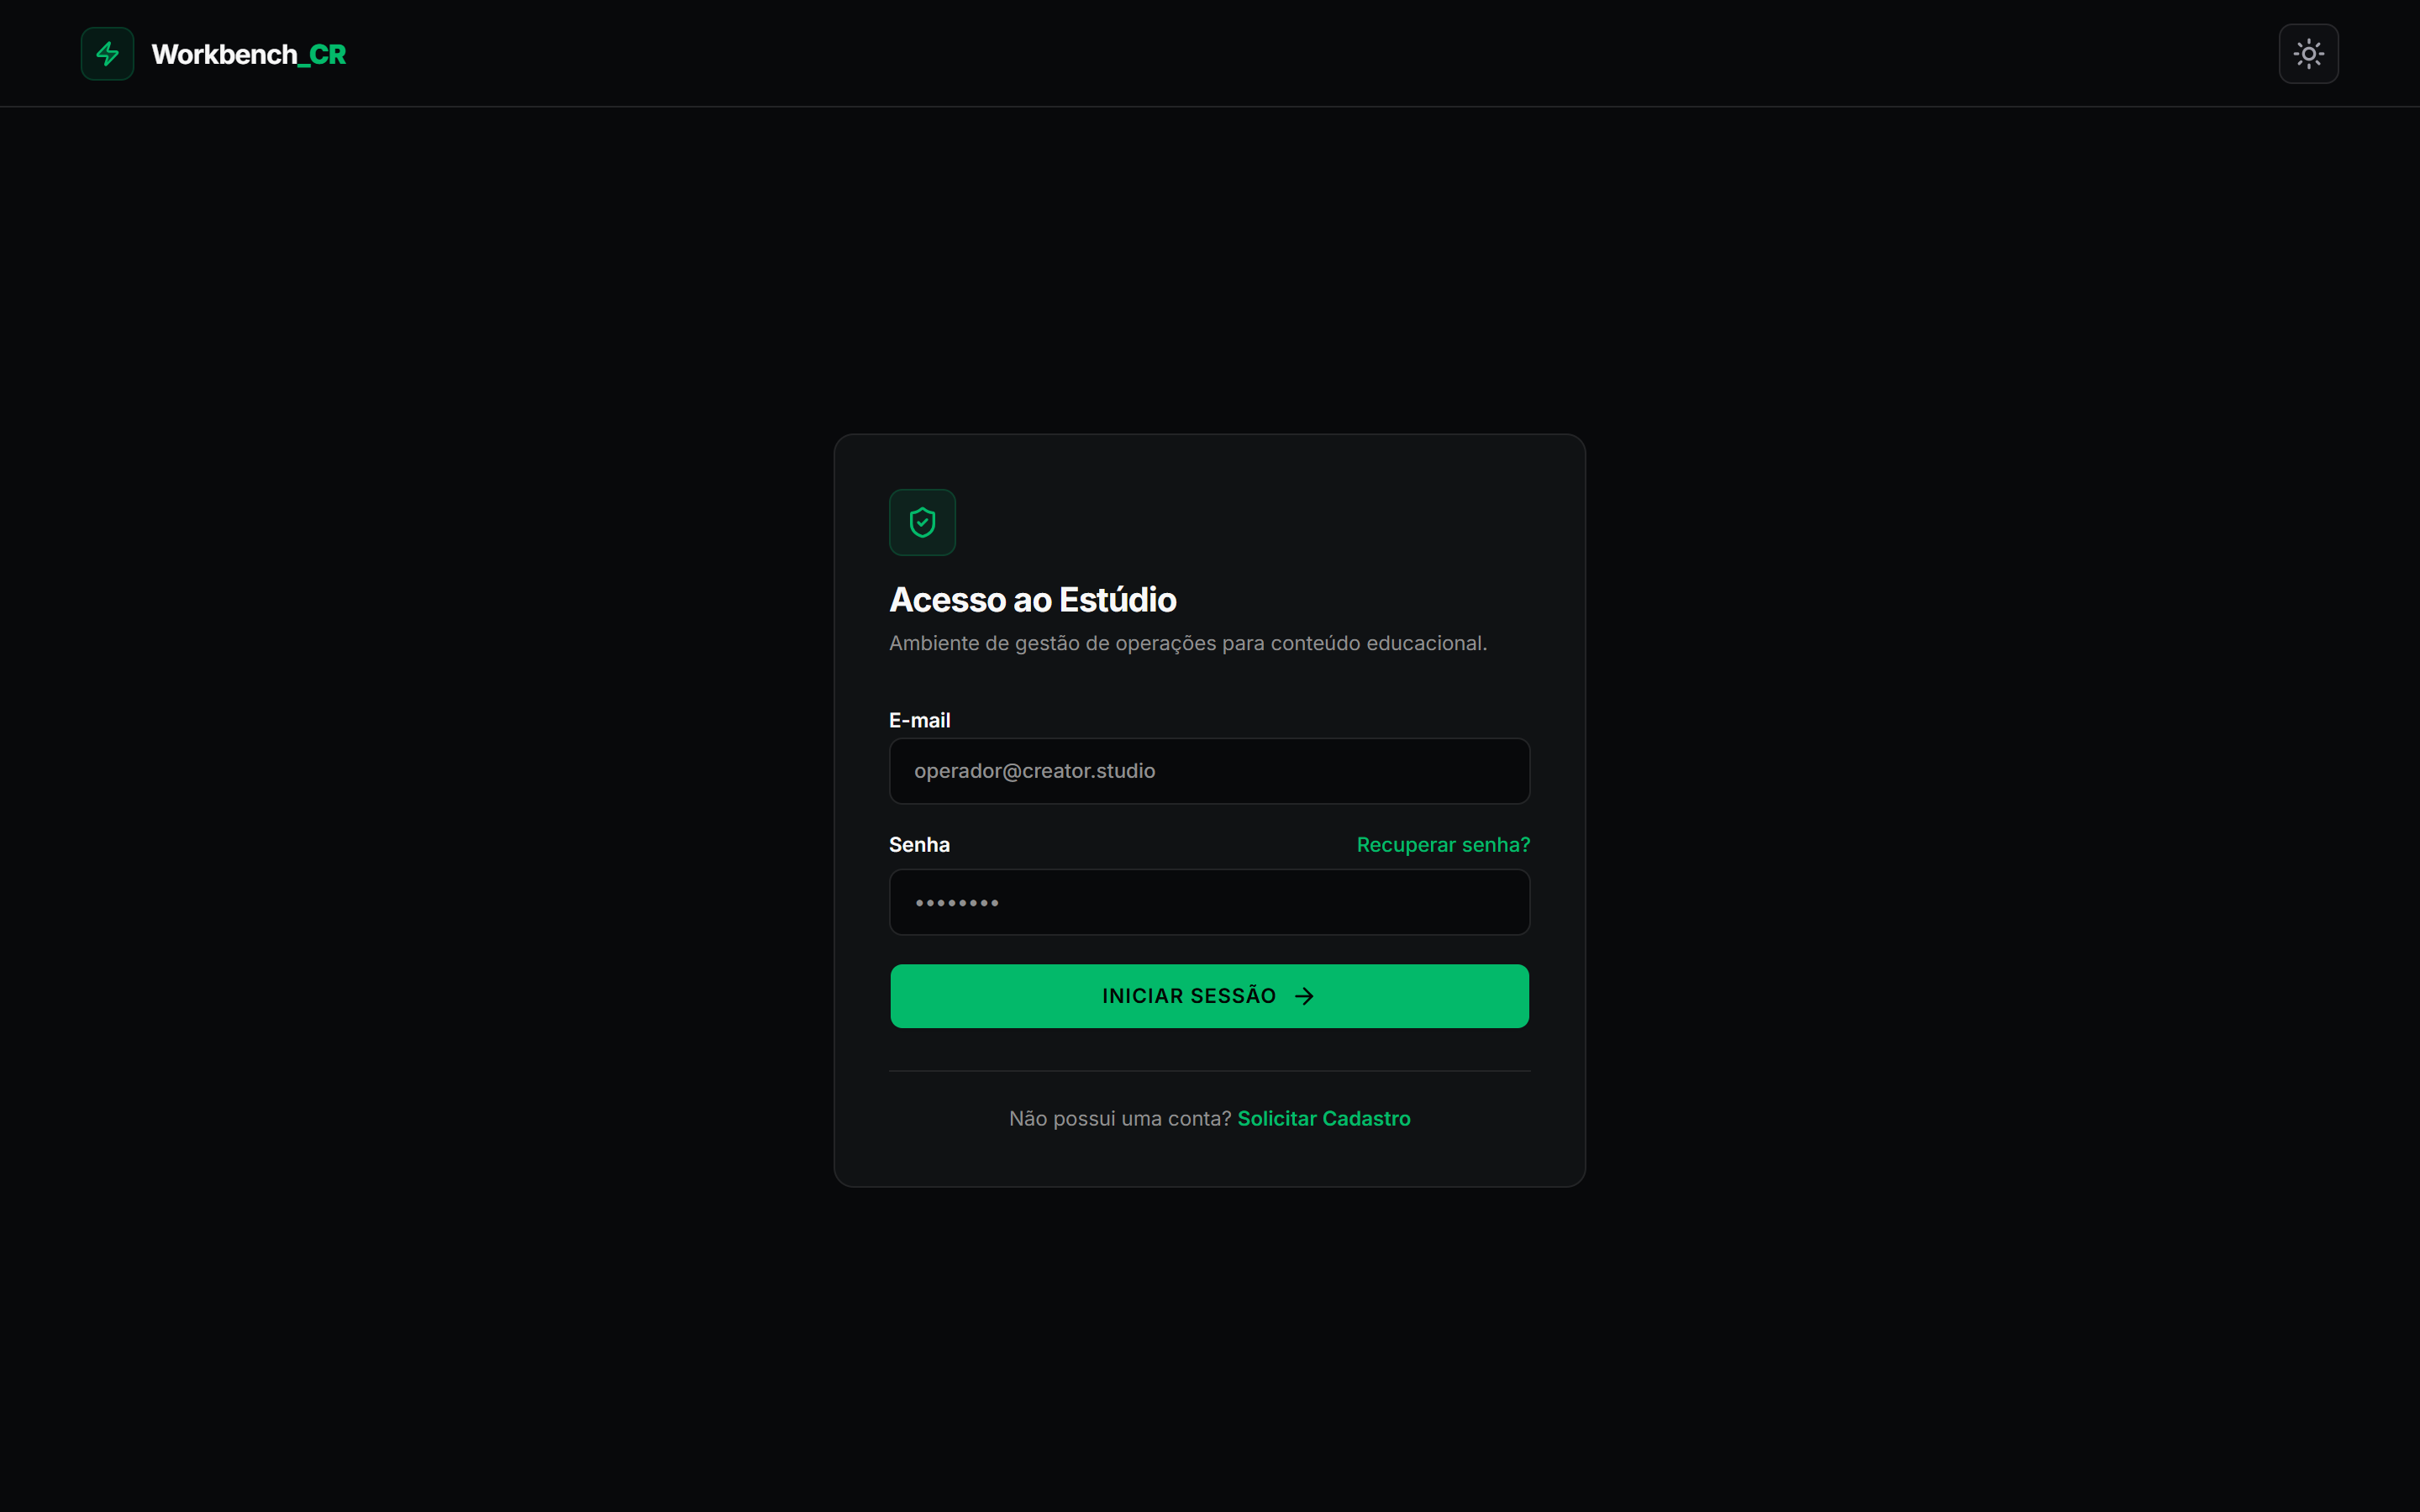
\includegraphics[width=0.85\textwidth]{imagens/01-login.png}
    \legend{Fonte: Produzido pelos autores.}
\end{figure}

\begin{figure}[H]
    \centering
    \caption{Recuperação de senha, com envio de um código de 6 dígitos para o e-mail cadastrado}
    \label{fig:tela-02}
    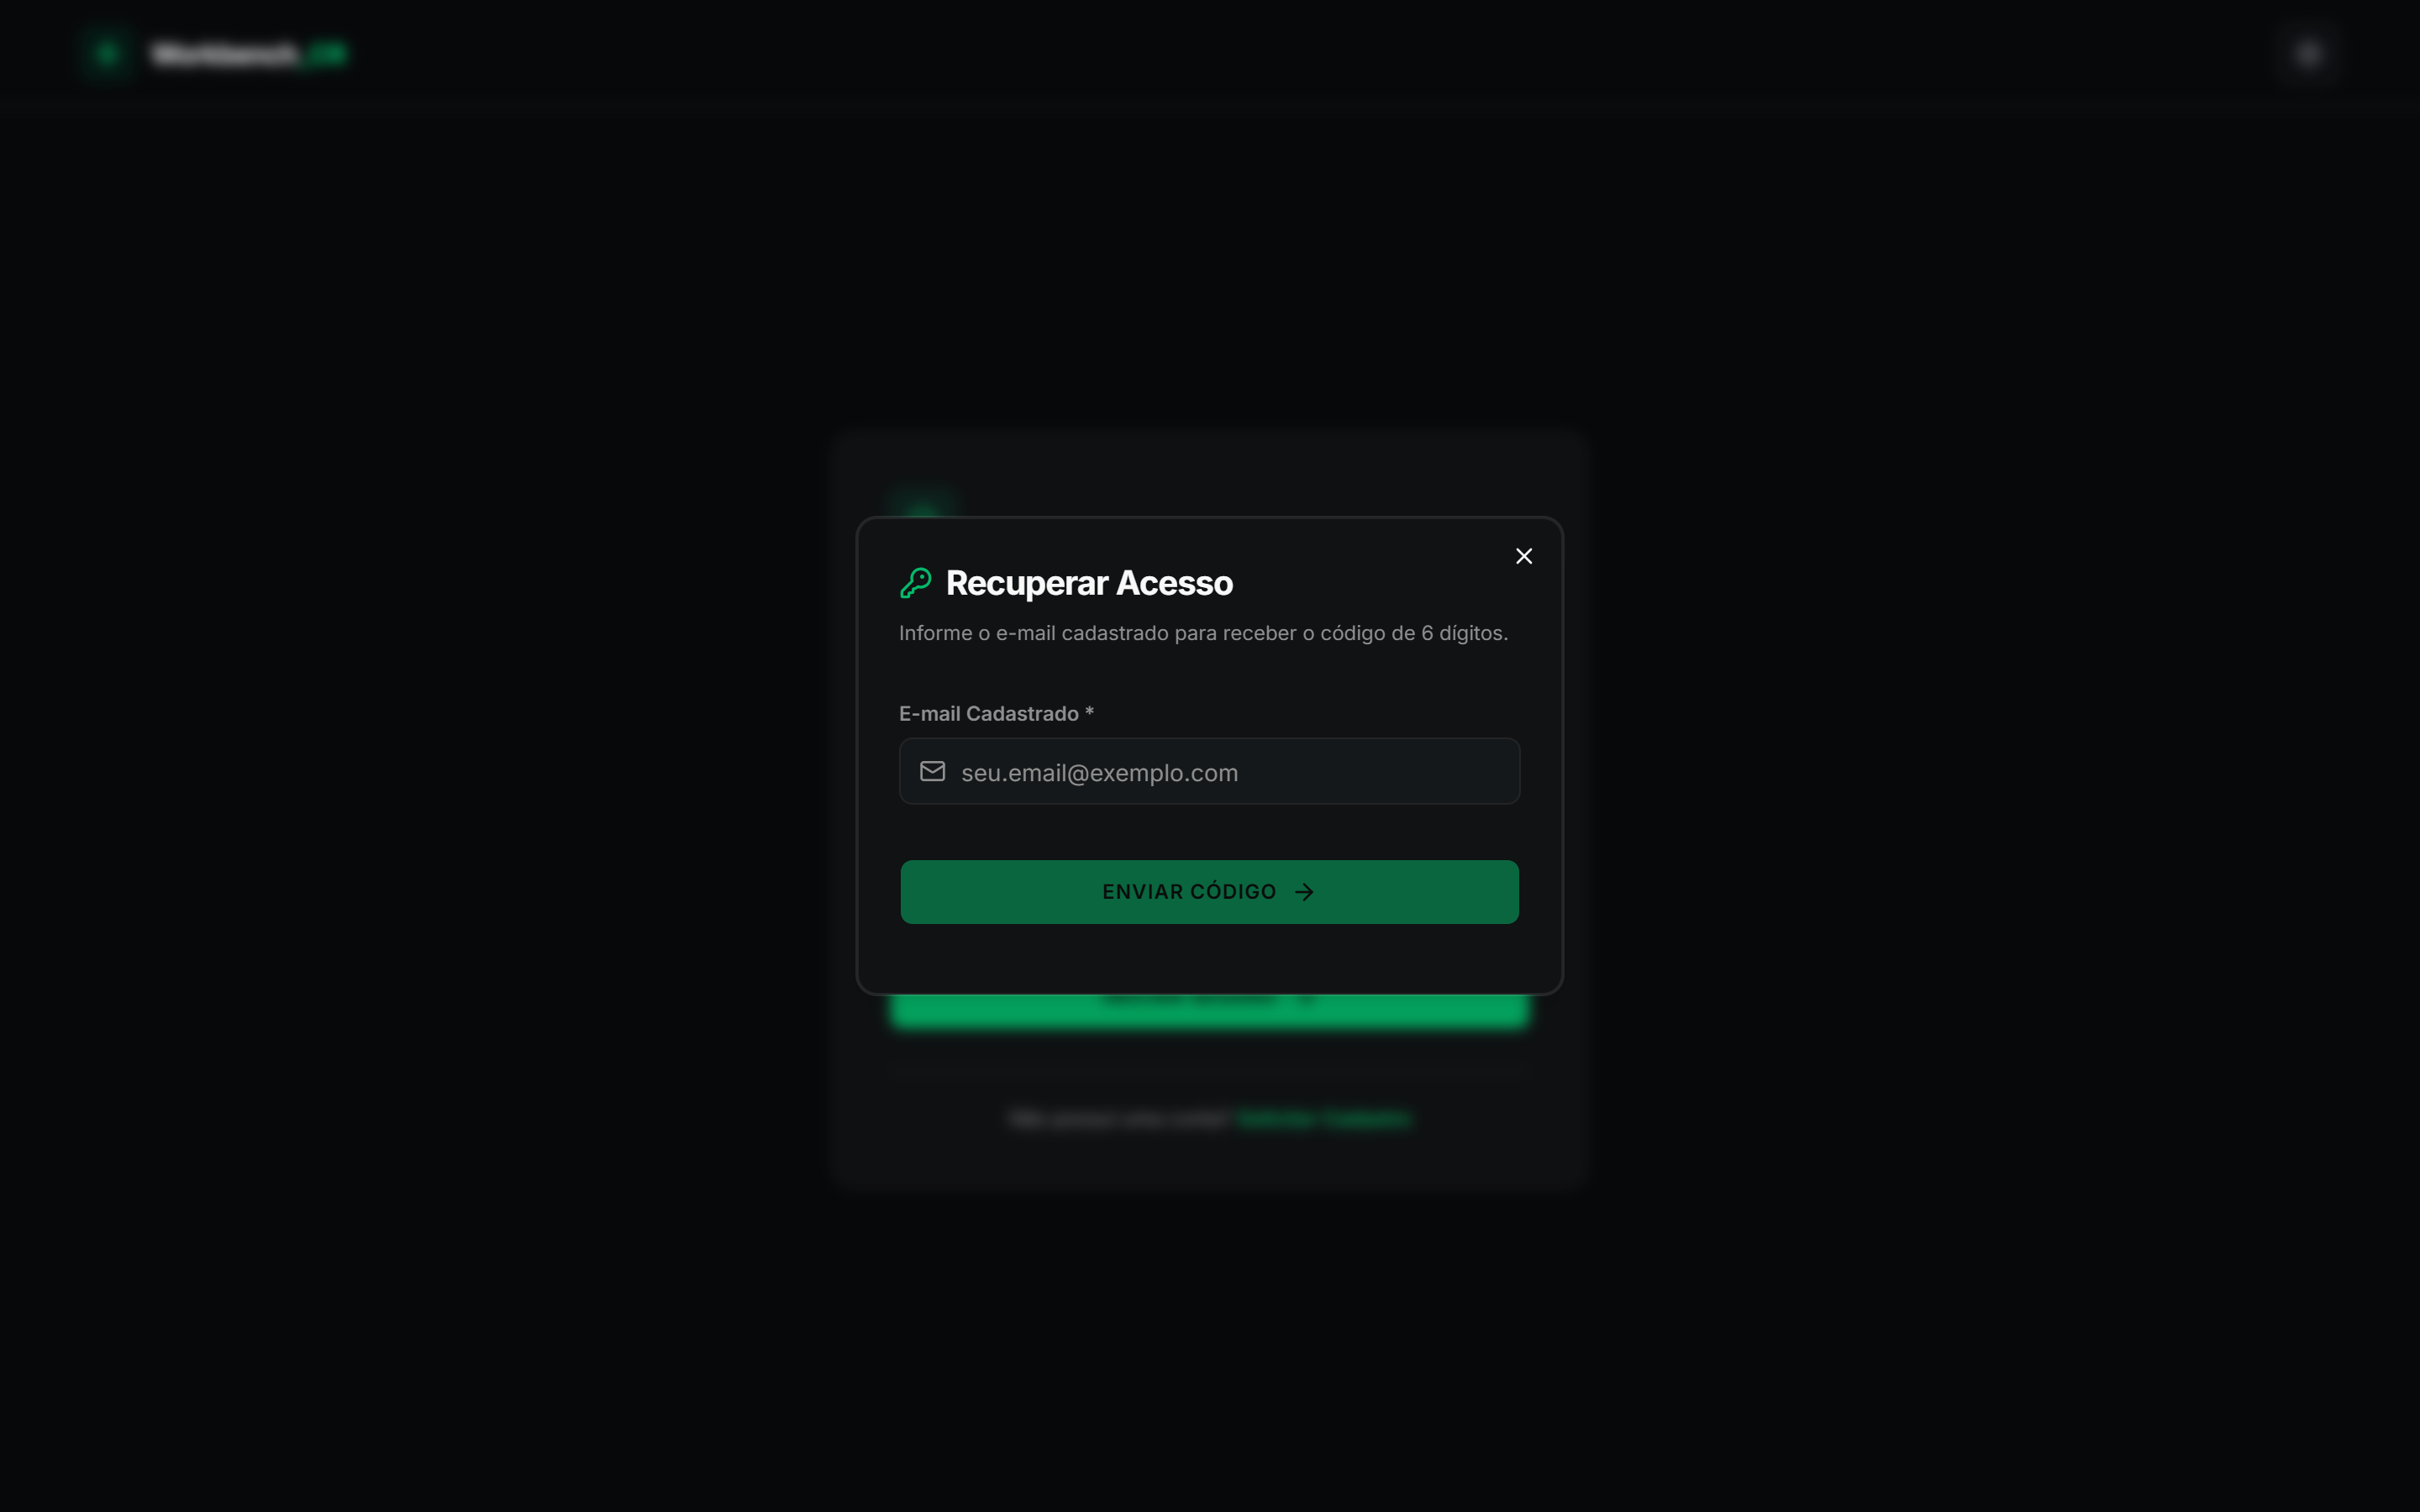
\includegraphics[width=0.85\textwidth]{imagens/02-recuperacao-de-senha.png}
    \legend{Fonte: Produzido pelos autores.}
\end{figure}

\begin{figure}[H]
    \centering
    \caption{Primeira etapa do cadastro, em que o usuário informa nome e e-mail para receber o código de acesso}
    \label{fig:tela-03}
    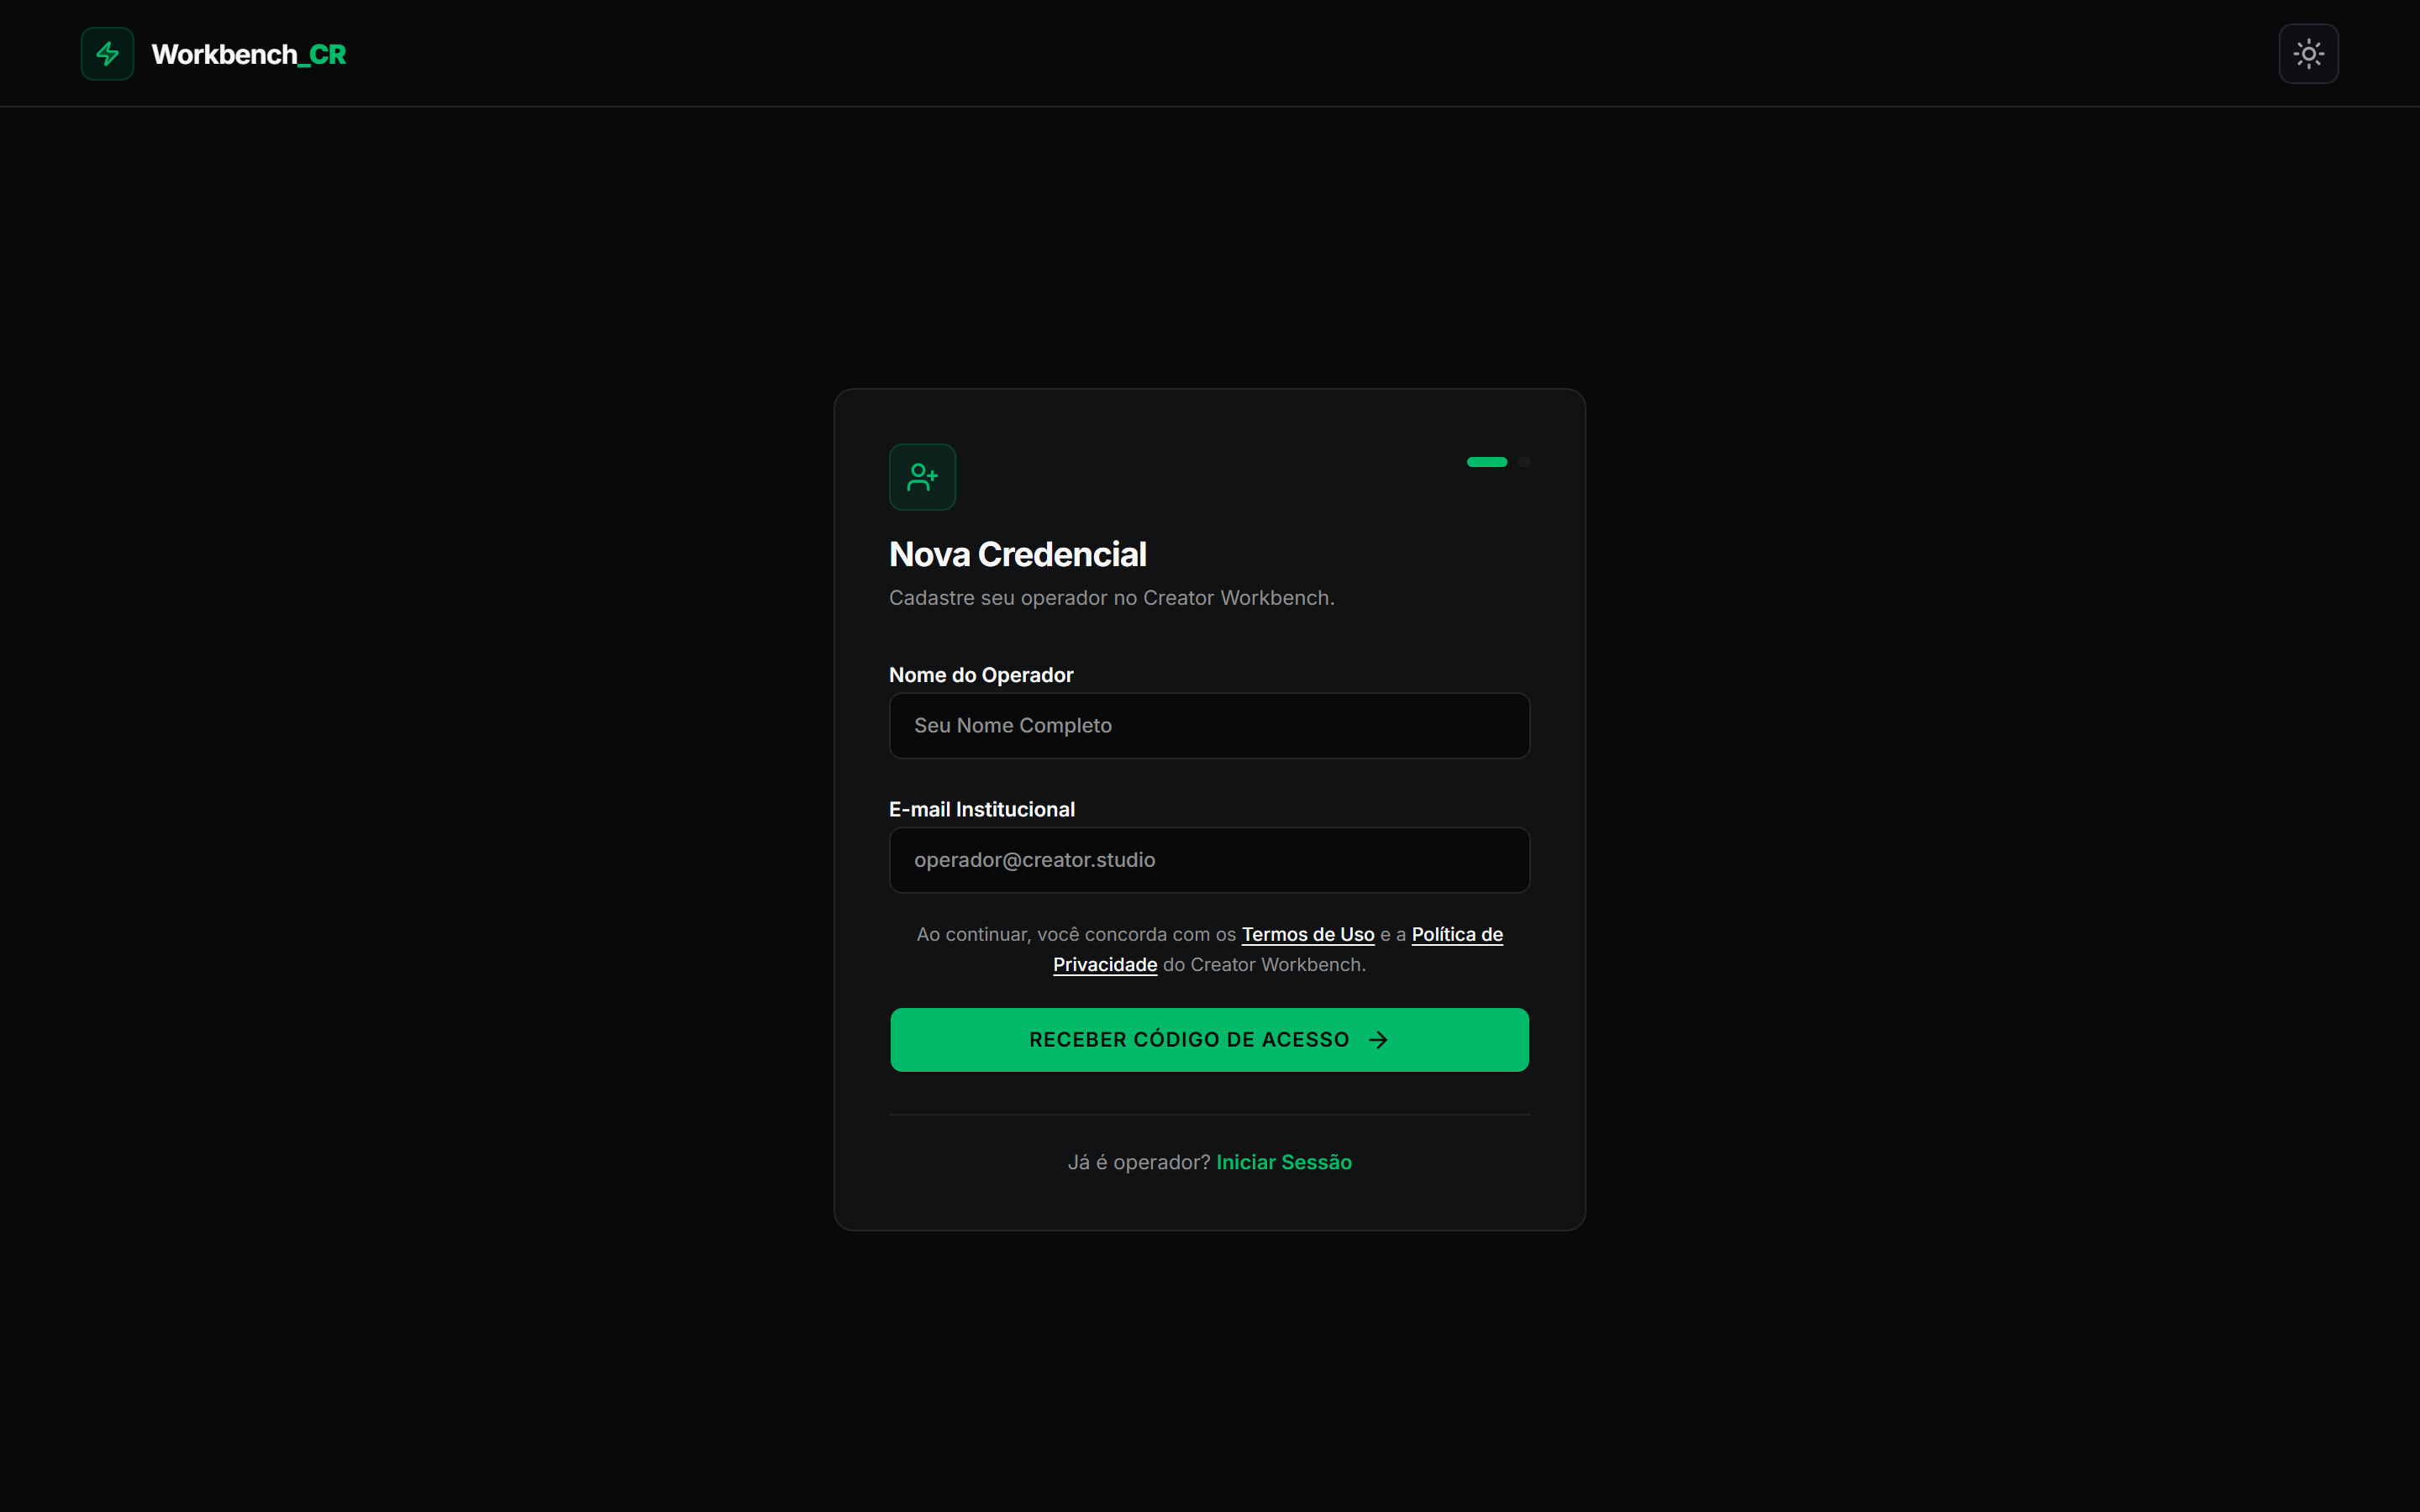
\includegraphics[width=0.85\textwidth]{imagens/03-cadastro.png}
    \legend{Fonte: Produzido pelos autores.}
\end{figure}

\begin{figure}[H]
    \centering
    \caption{Página de convite (\texttt{/convite}), com a equipe, o papel oferecido e o e-mail do convidado}
    \label{fig:tela-04}
    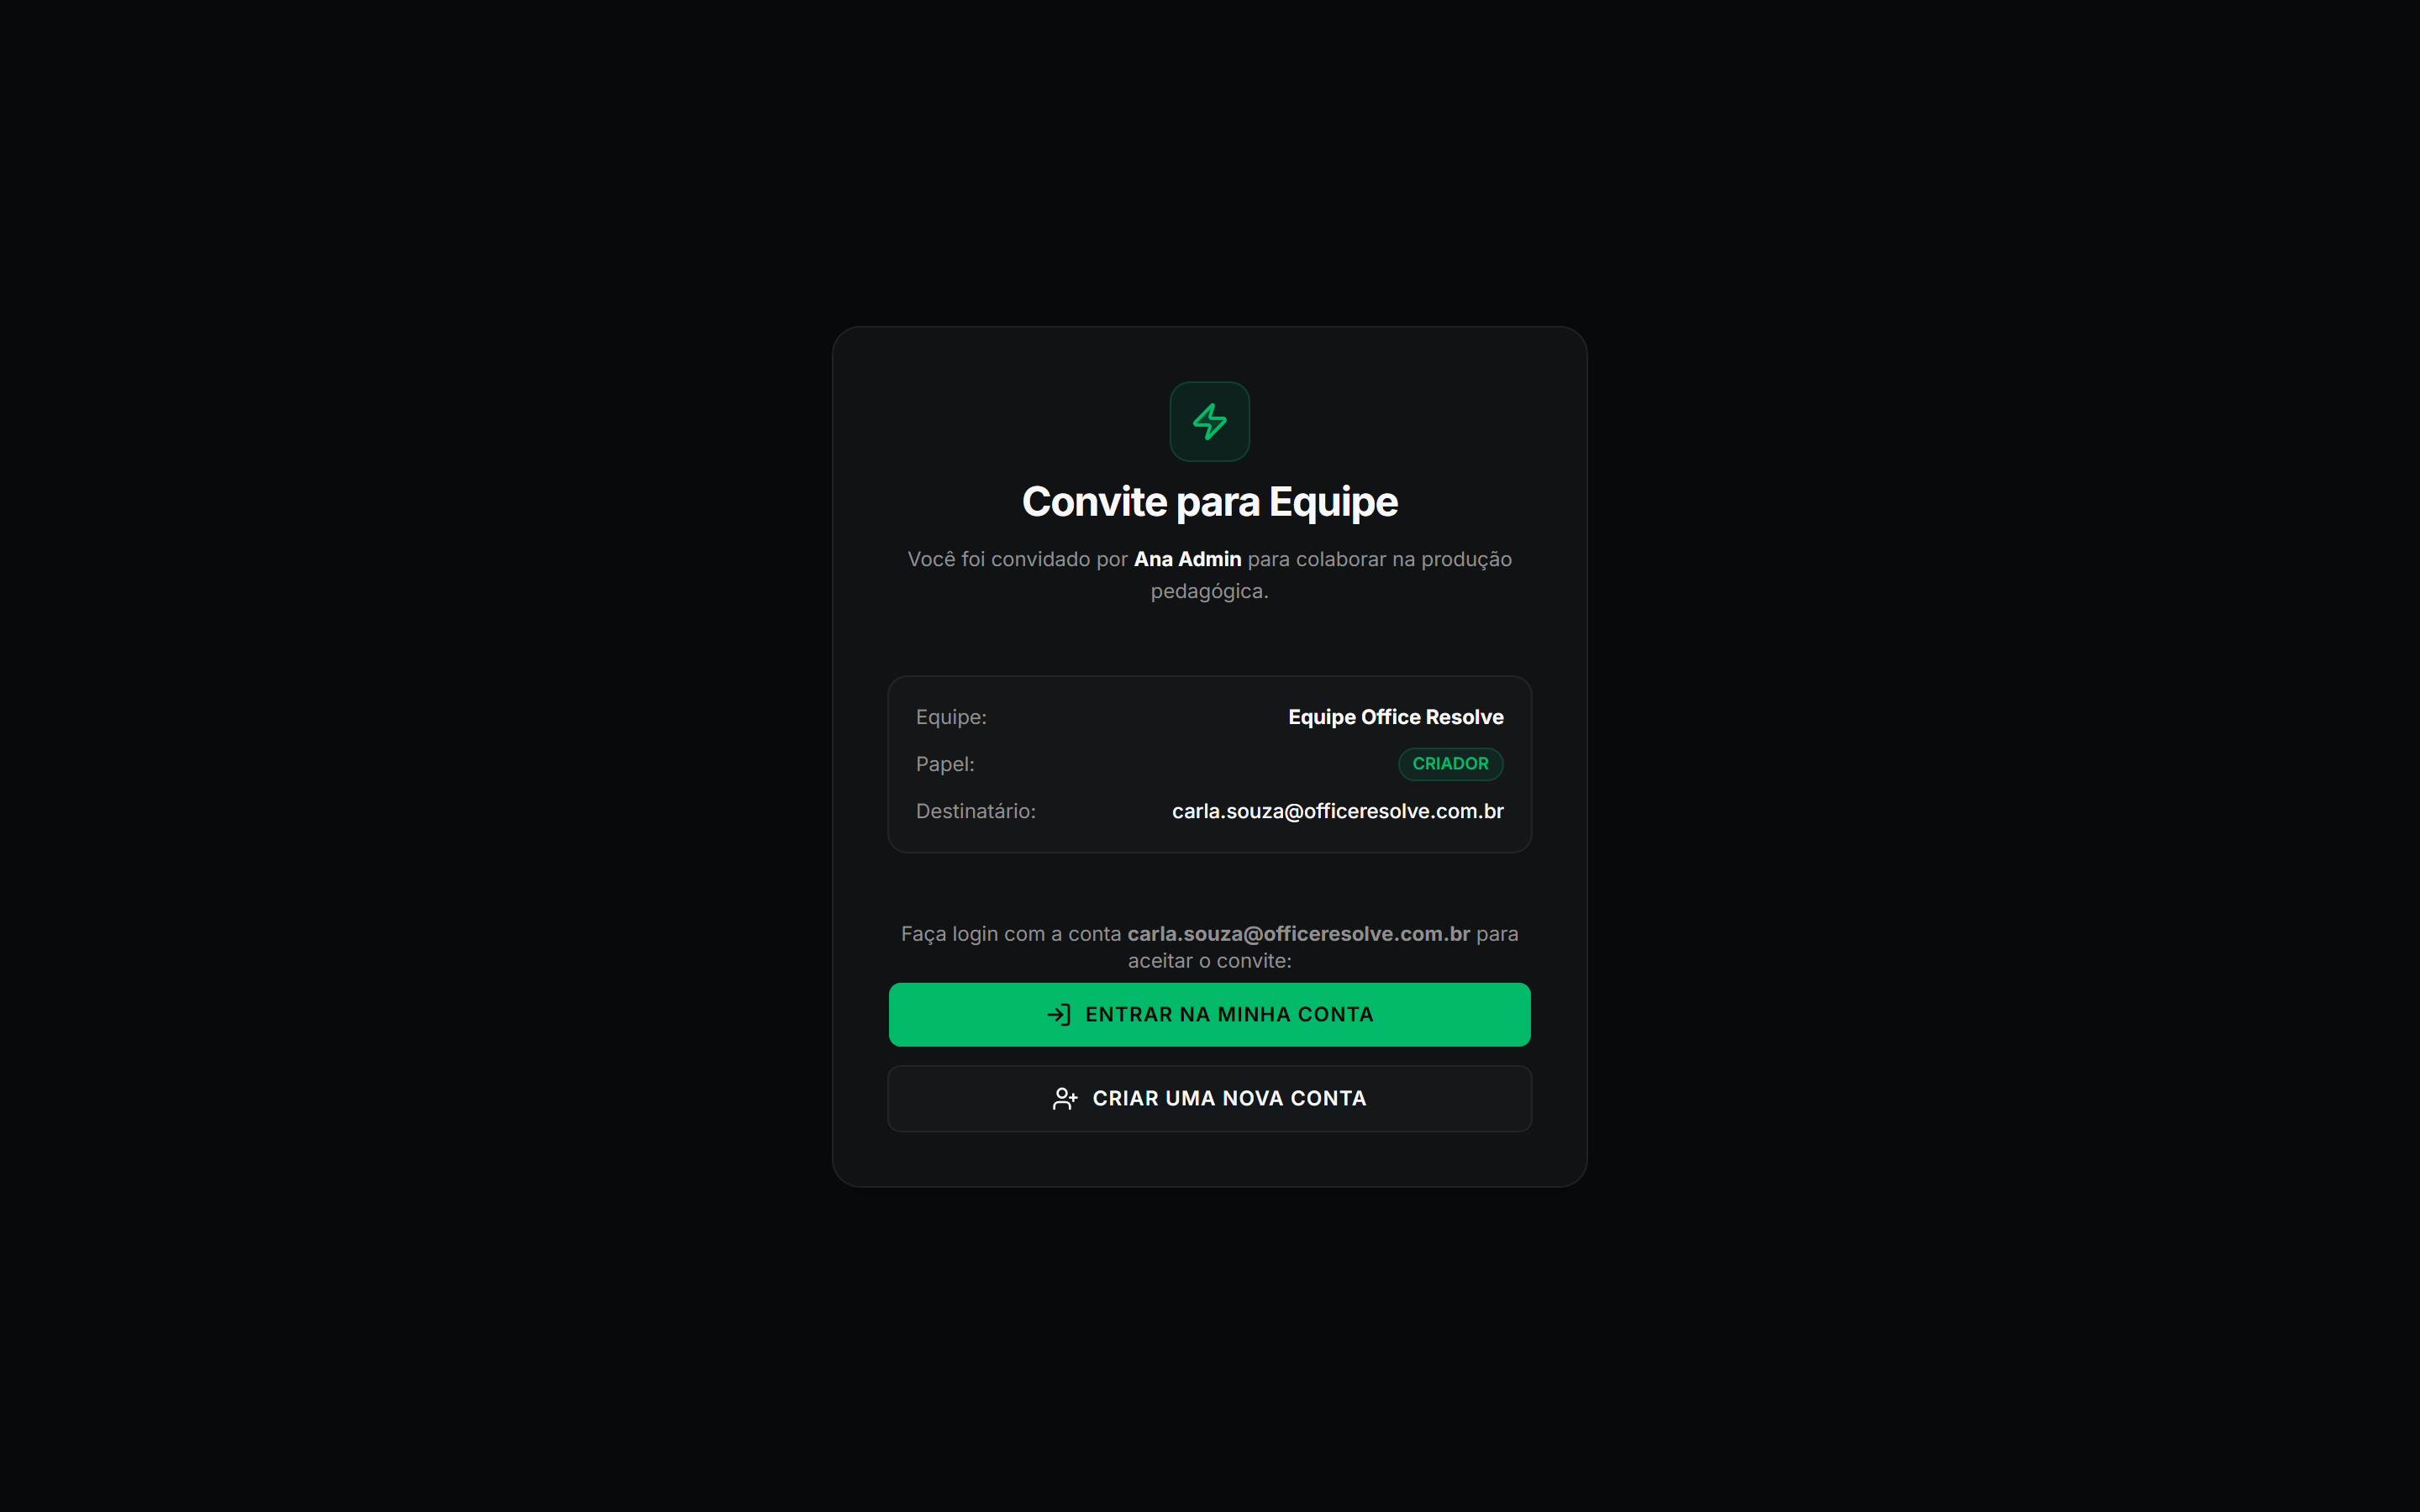
\includegraphics[width=0.85\textwidth]{imagens/04-convite-para-equipe.png}
    \legend{Fonte: Produzido pelos autores.}
\end{figure}

\section{Painel e quadro de produção}

\begin{figure}[H]
    \centering
    \caption{Painel de Controle com o quadro \textit{Kanban} da equipe, em colunas configuráveis, com prazos e progresso das tarefas de cada projeto}
    \label{fig:tela-05}
    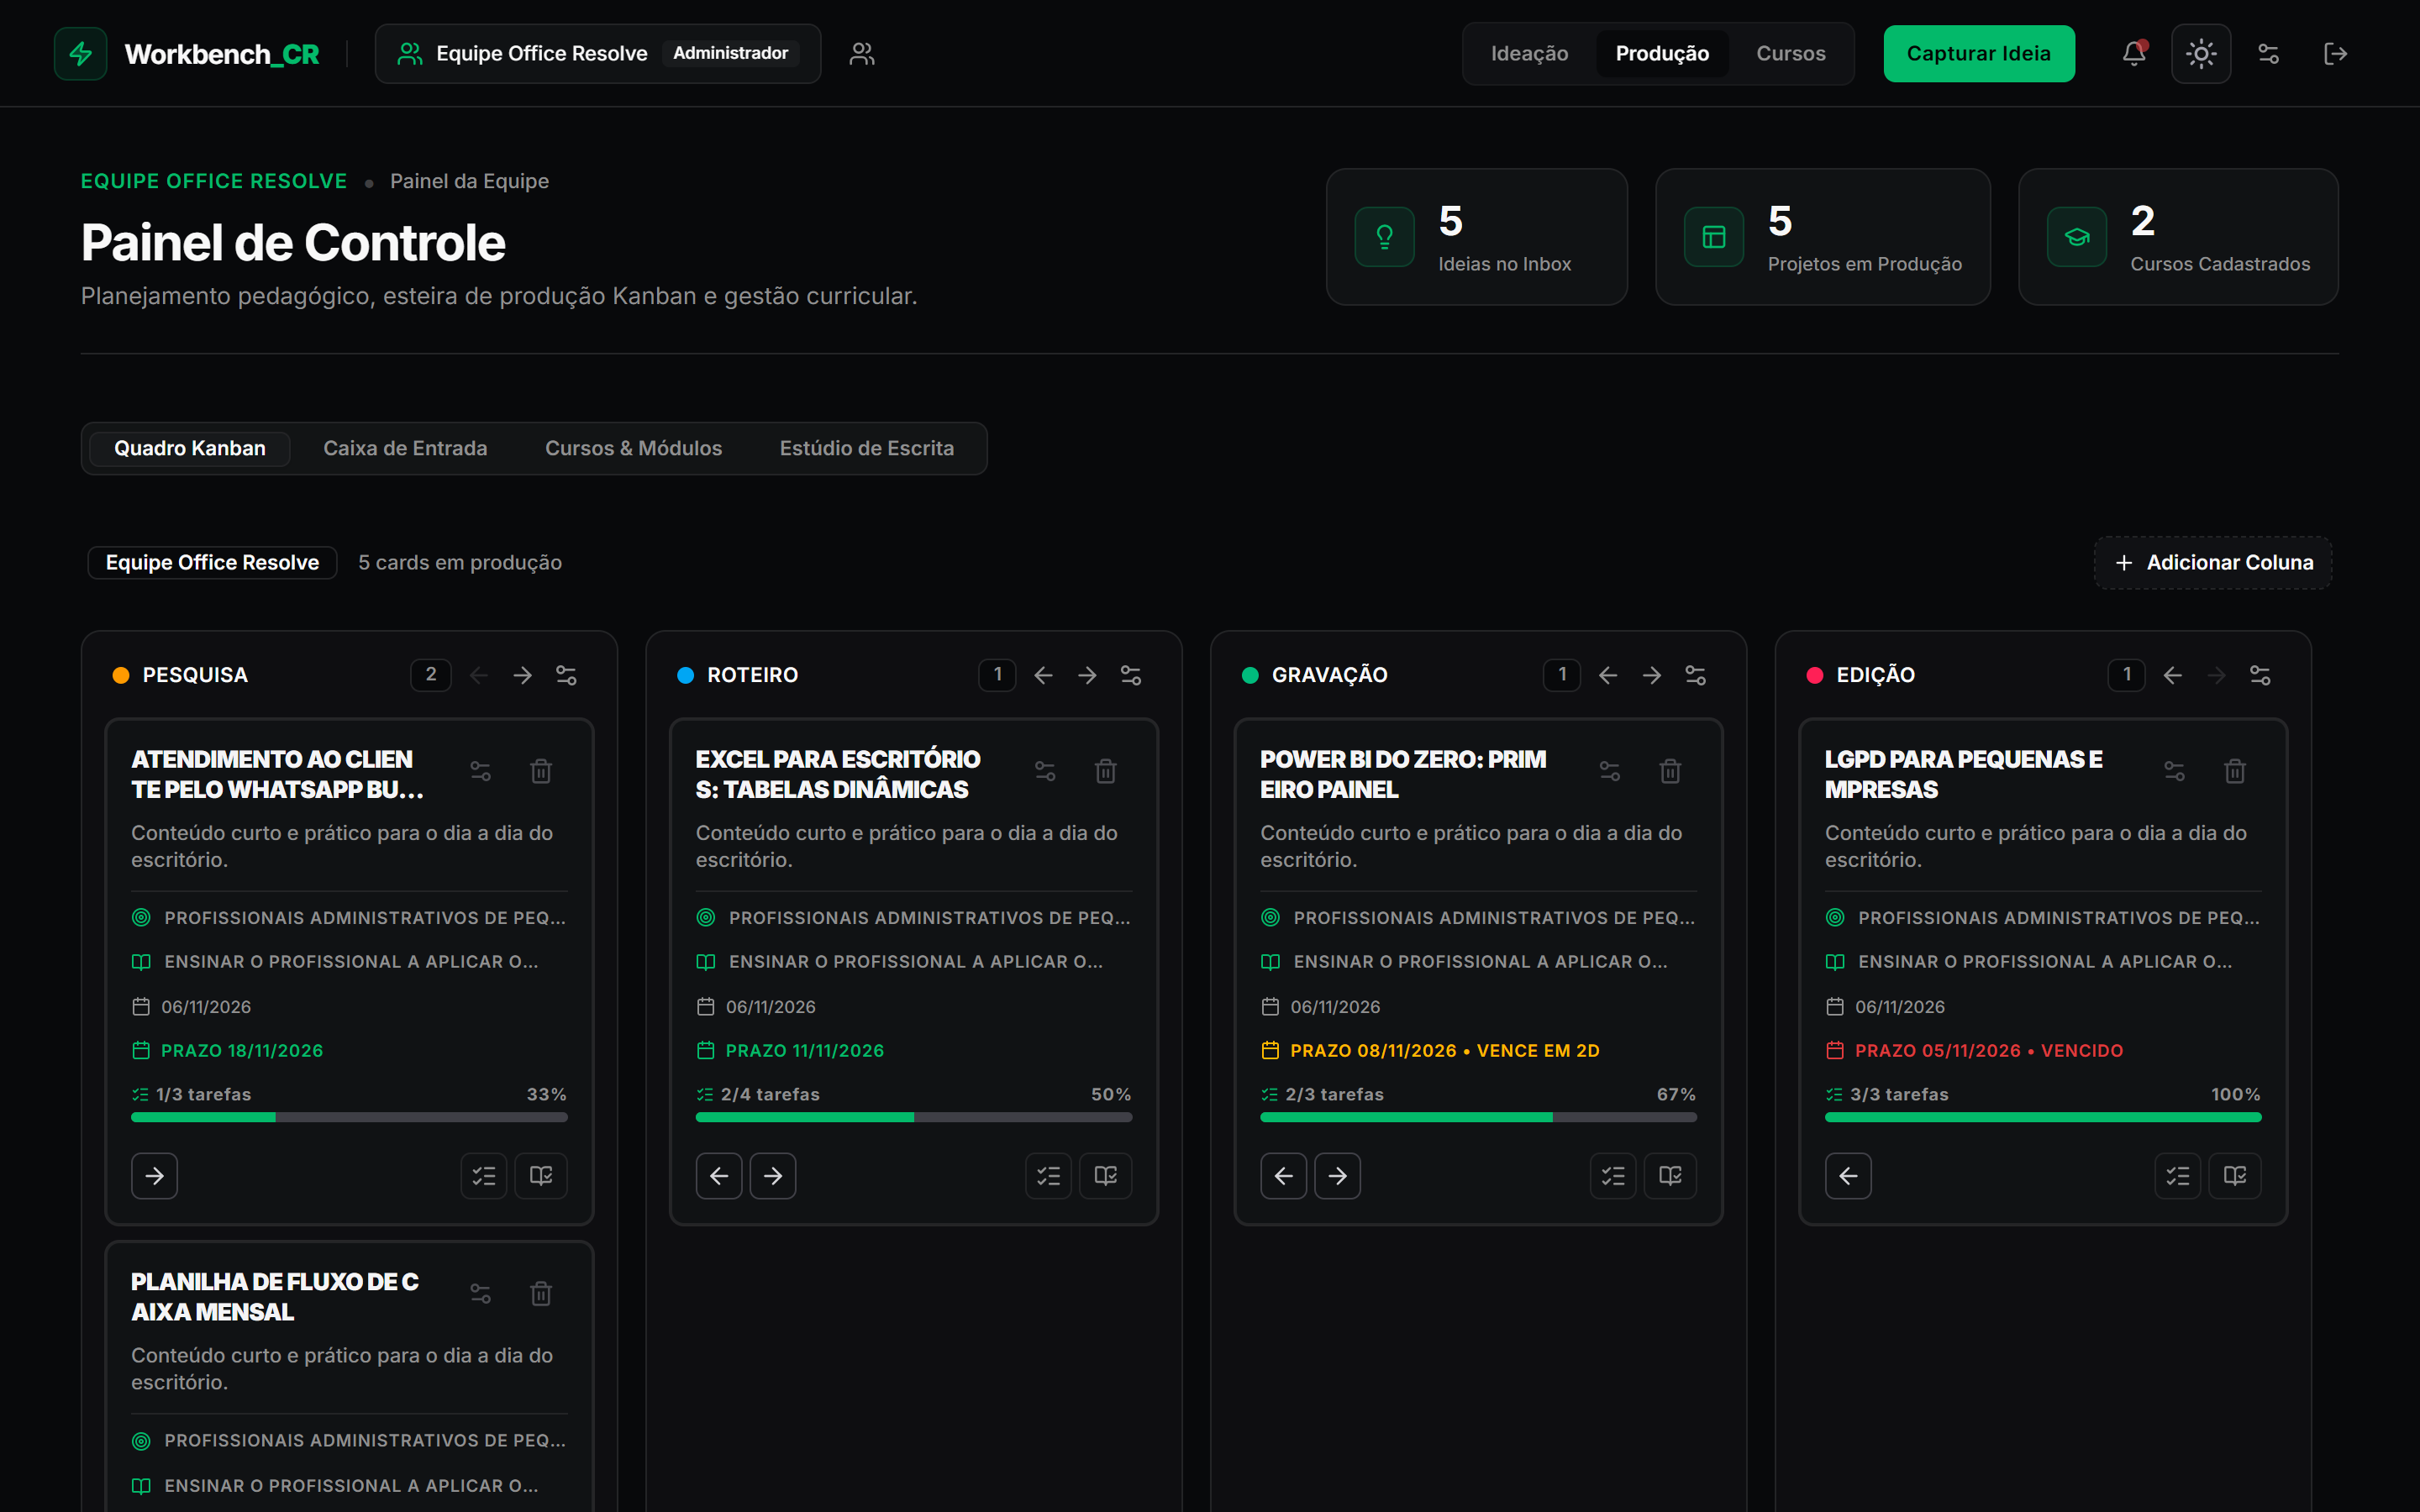
\includegraphics[width=0.85\textwidth]{imagens/05-painel-quadro-kanban.png}
    \legend{Fonte: Produzido pelos autores.}
\end{figure}

\begin{figure}[H]
    \centering
    \caption{Painel de alertas de prazo, com os projetos e as tarefas atrasados ou que vencem nos próximos dias (RF09)}
    \label{fig:tela-06}
    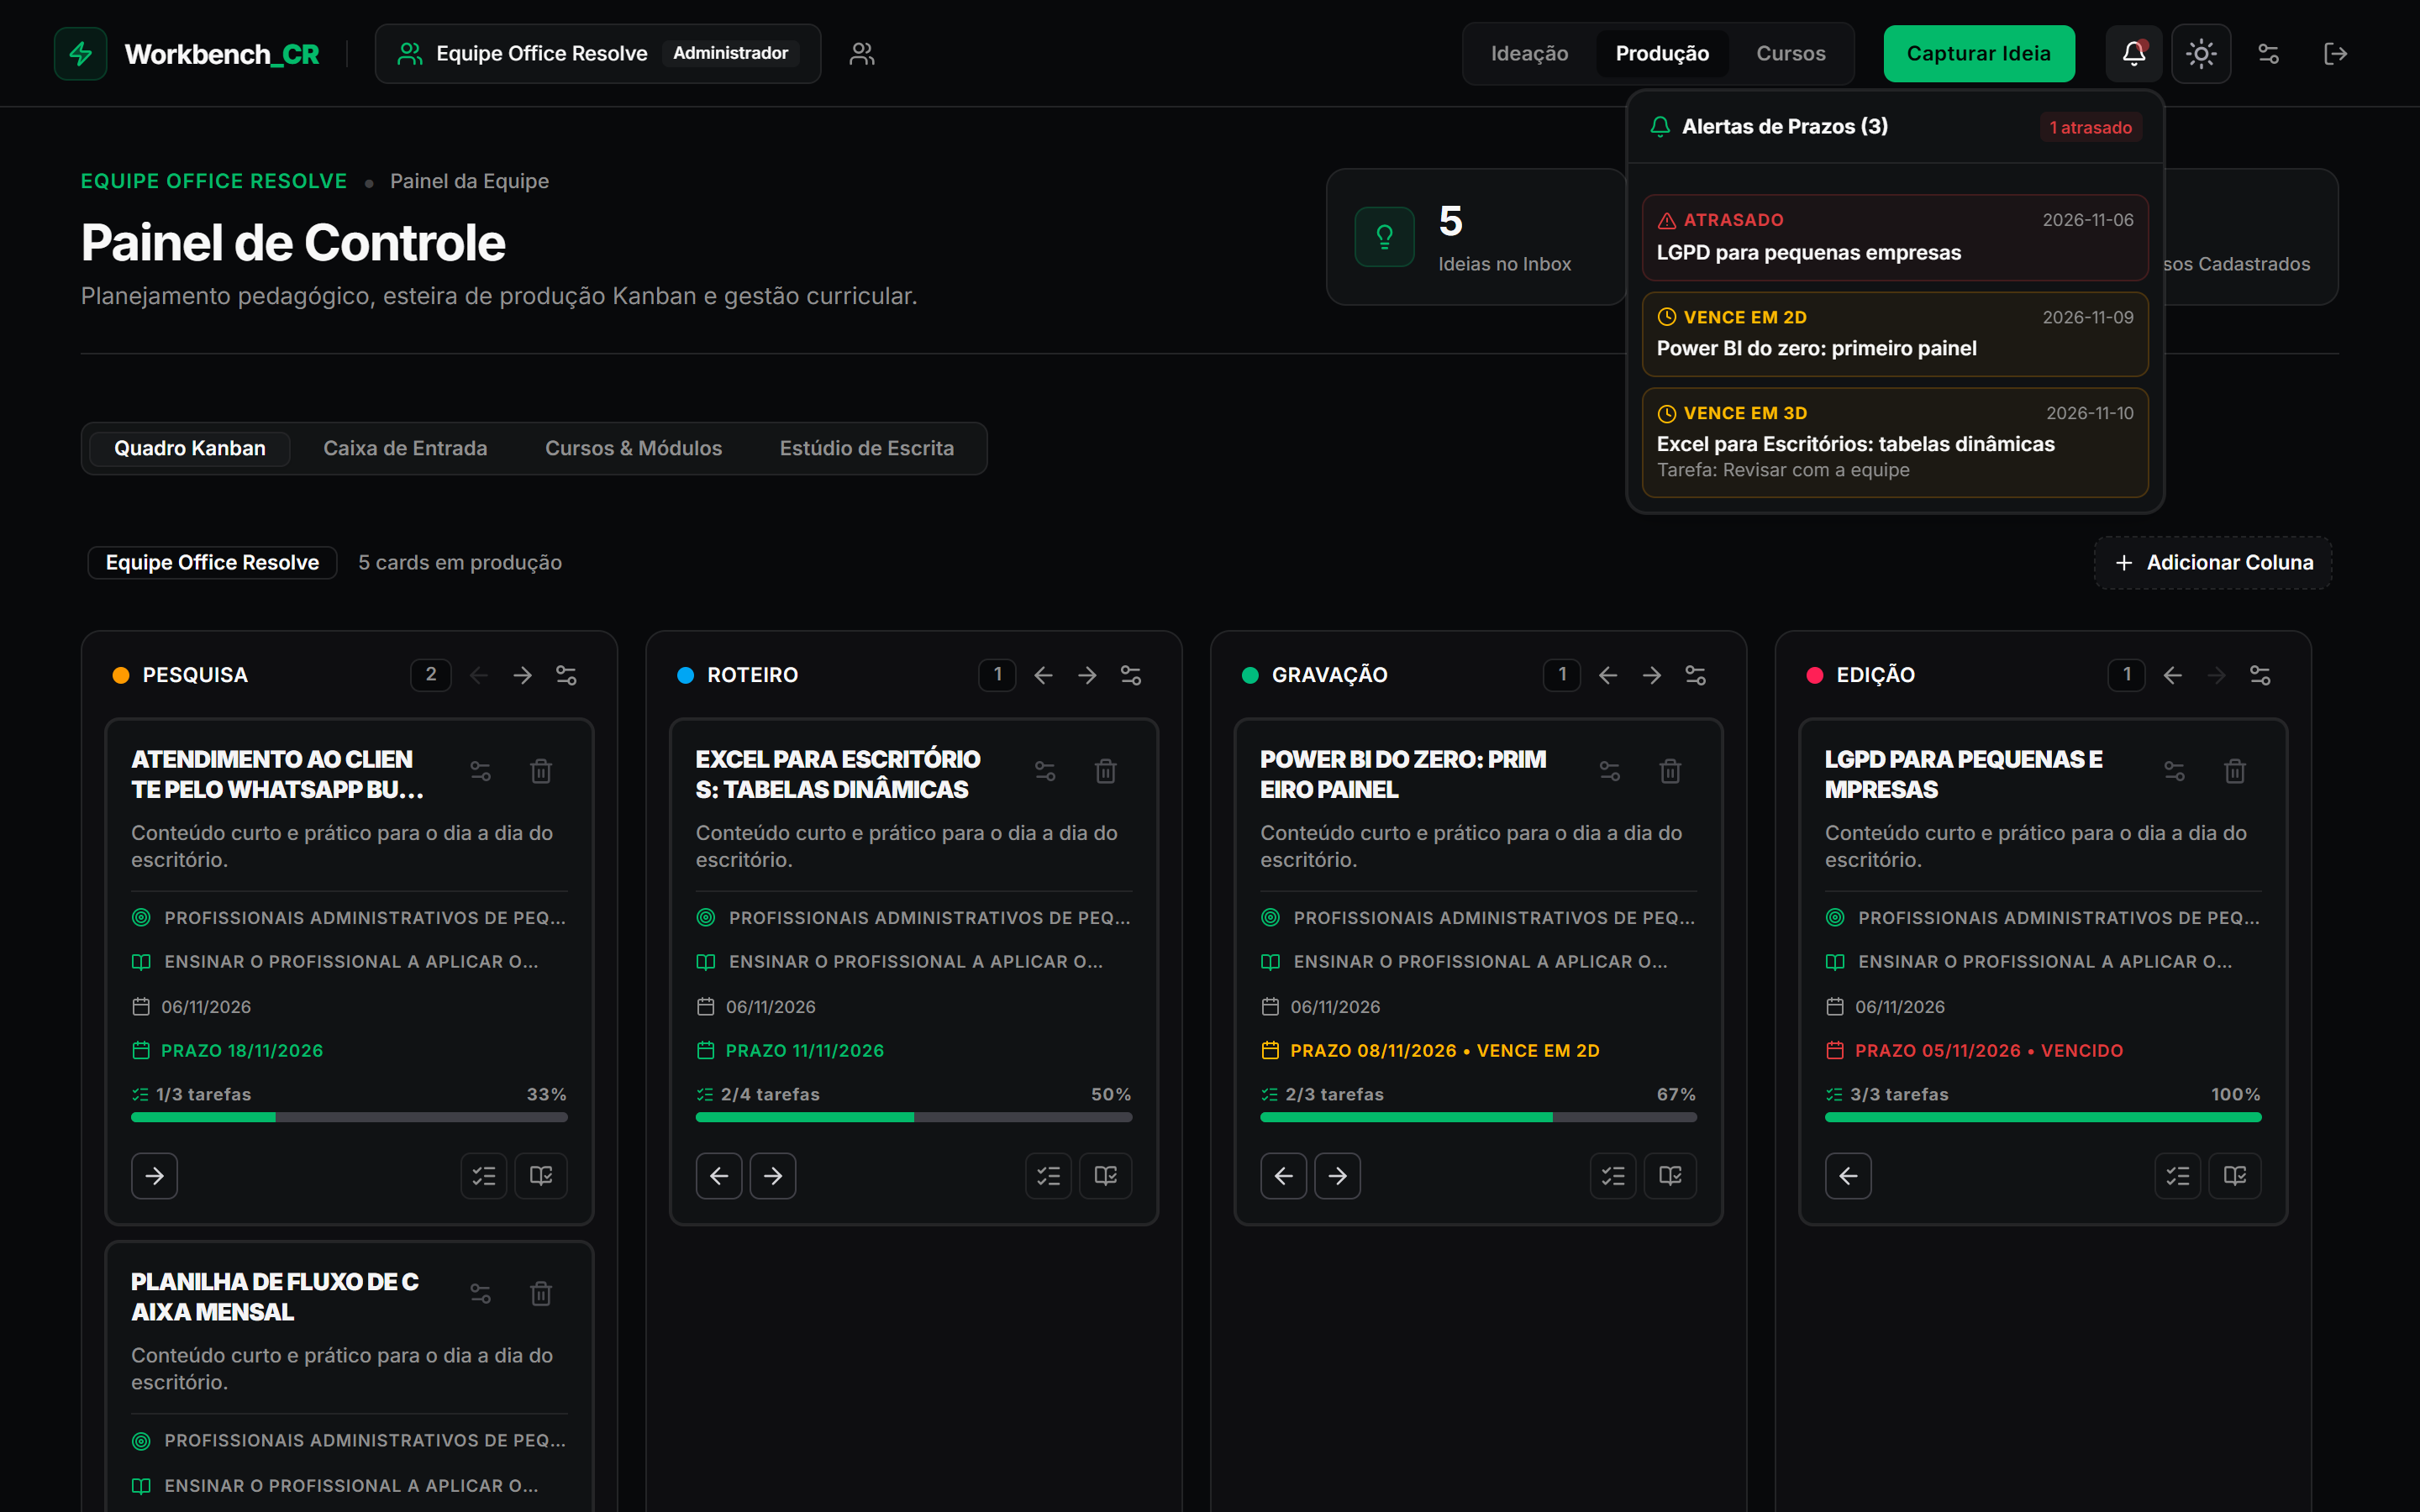
\includegraphics[width=0.85\textwidth]{imagens/06-alertas-de-prazo.png}
    \legend{Fonte: Produzido pelos autores.}
\end{figure}

\section{Ideias}

\begin{figure}[H]
    \centering
    \caption{Caixa de Entrada de ideias, com etiquetas, votos e botão para converter a ideia em projeto}
    \label{fig:tela-07}
    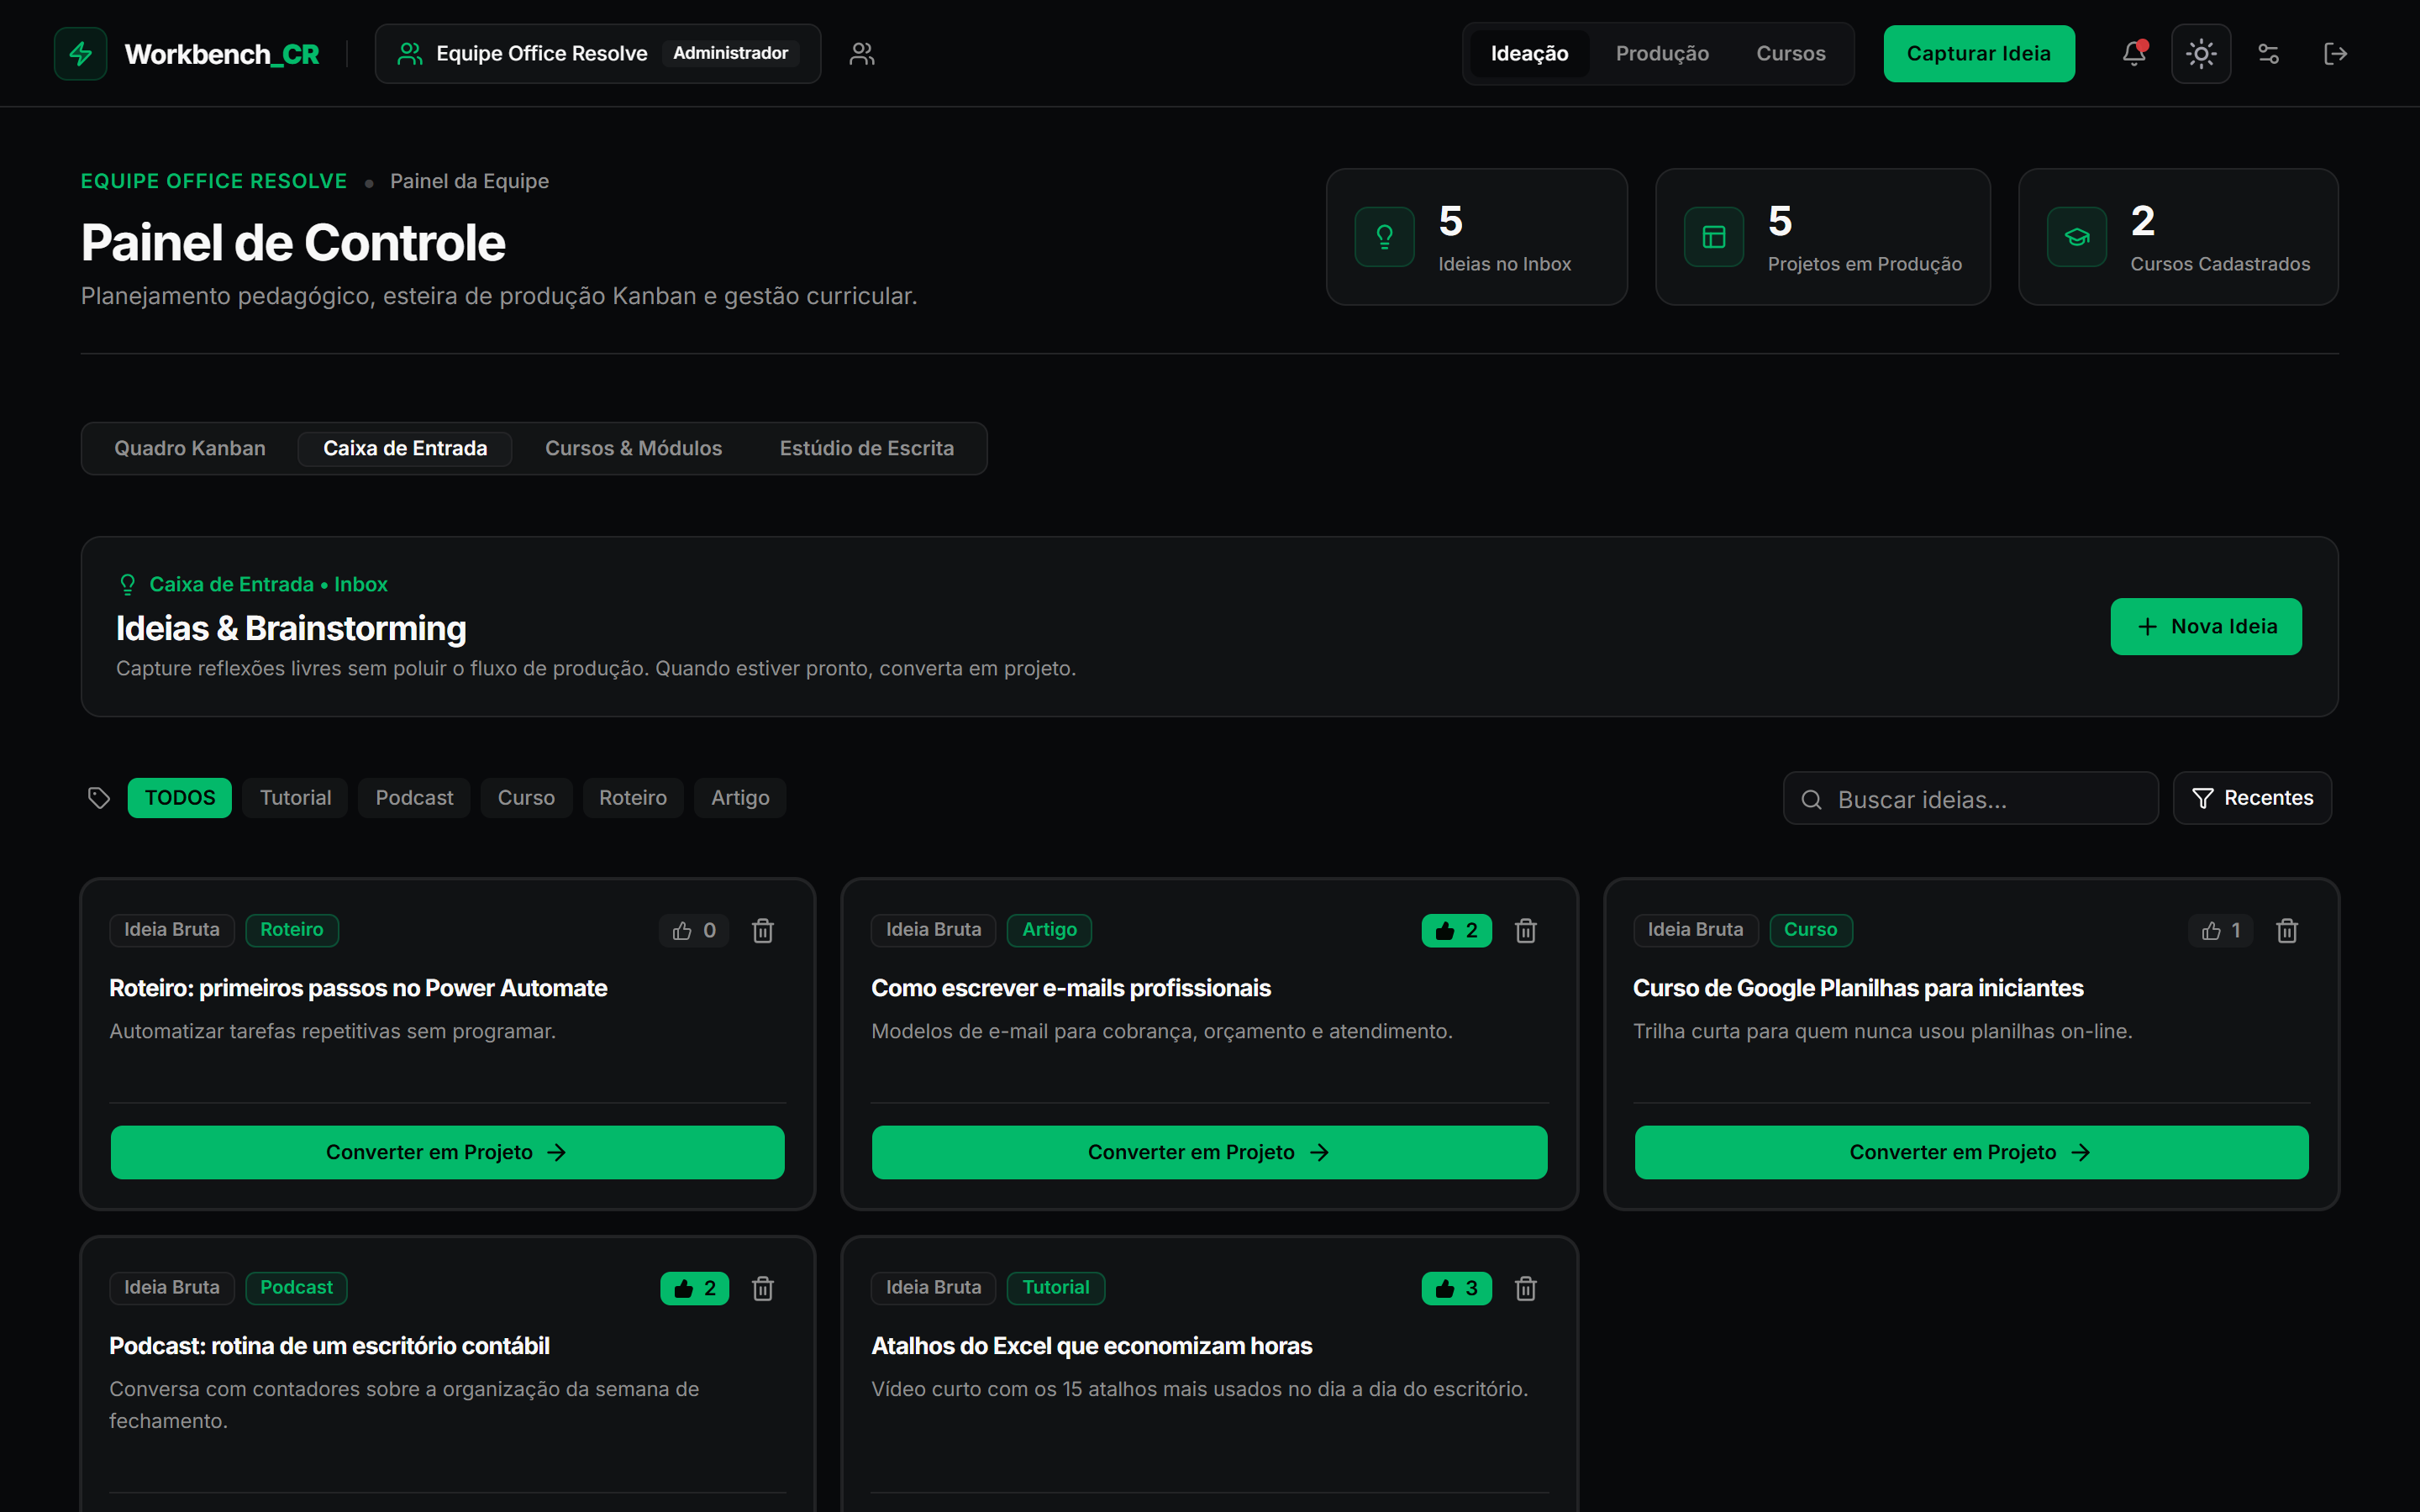
\includegraphics[width=0.85\textwidth]{imagens/07-caixa-de-entrada.png}
    \legend{Fonte: Produzido pelos autores.}
\end{figure}

\begin{figure}[H]
    \centering
    \caption{Captura de nova ideia, com título, descrição, público-alvo, objetivo pedagógico e etiqueta}
    \label{fig:tela-08}
    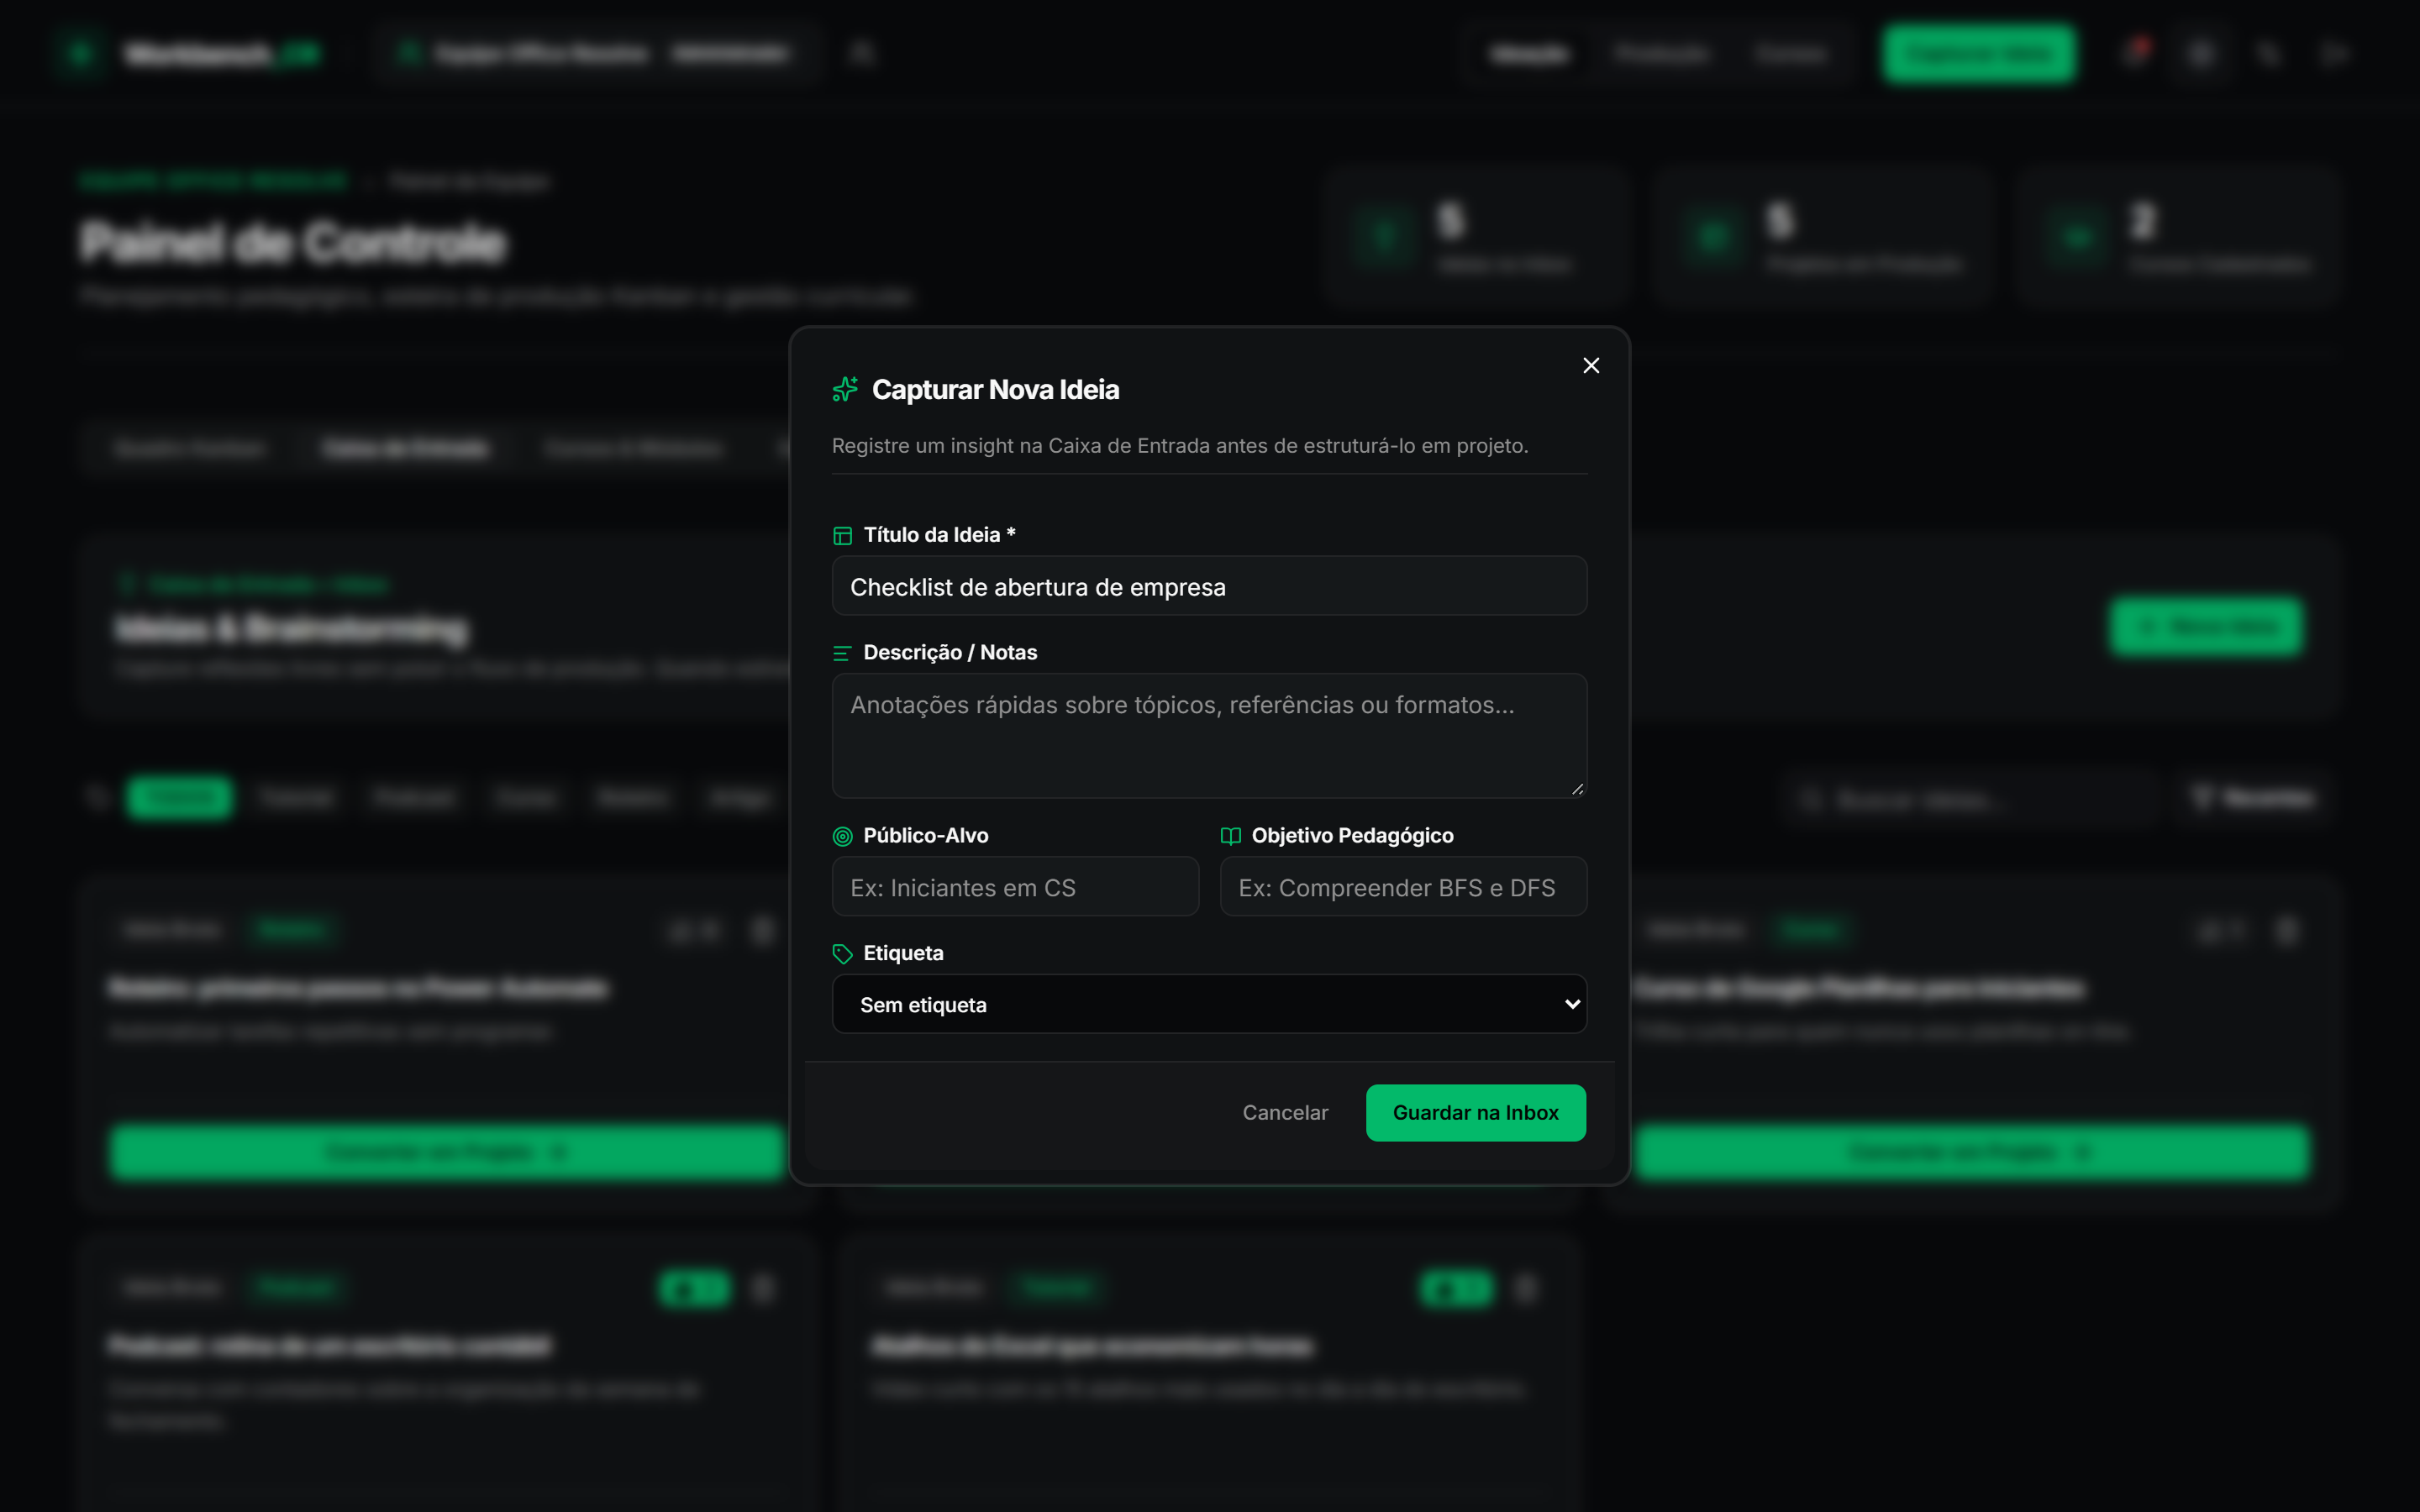
\includegraphics[width=0.85\textwidth]{imagens/08-nova-ideia.png}
    \legend{Fonte: Produzido pelos autores.}
\end{figure}

\begin{figure}[H]
    \centering
    \caption{Conversão de ideia em projeto, que exige público-alvo e objetivo pedagógico (RN01) e permite escolher a coluna inicial do quadro}
    \label{fig:tela-09}
    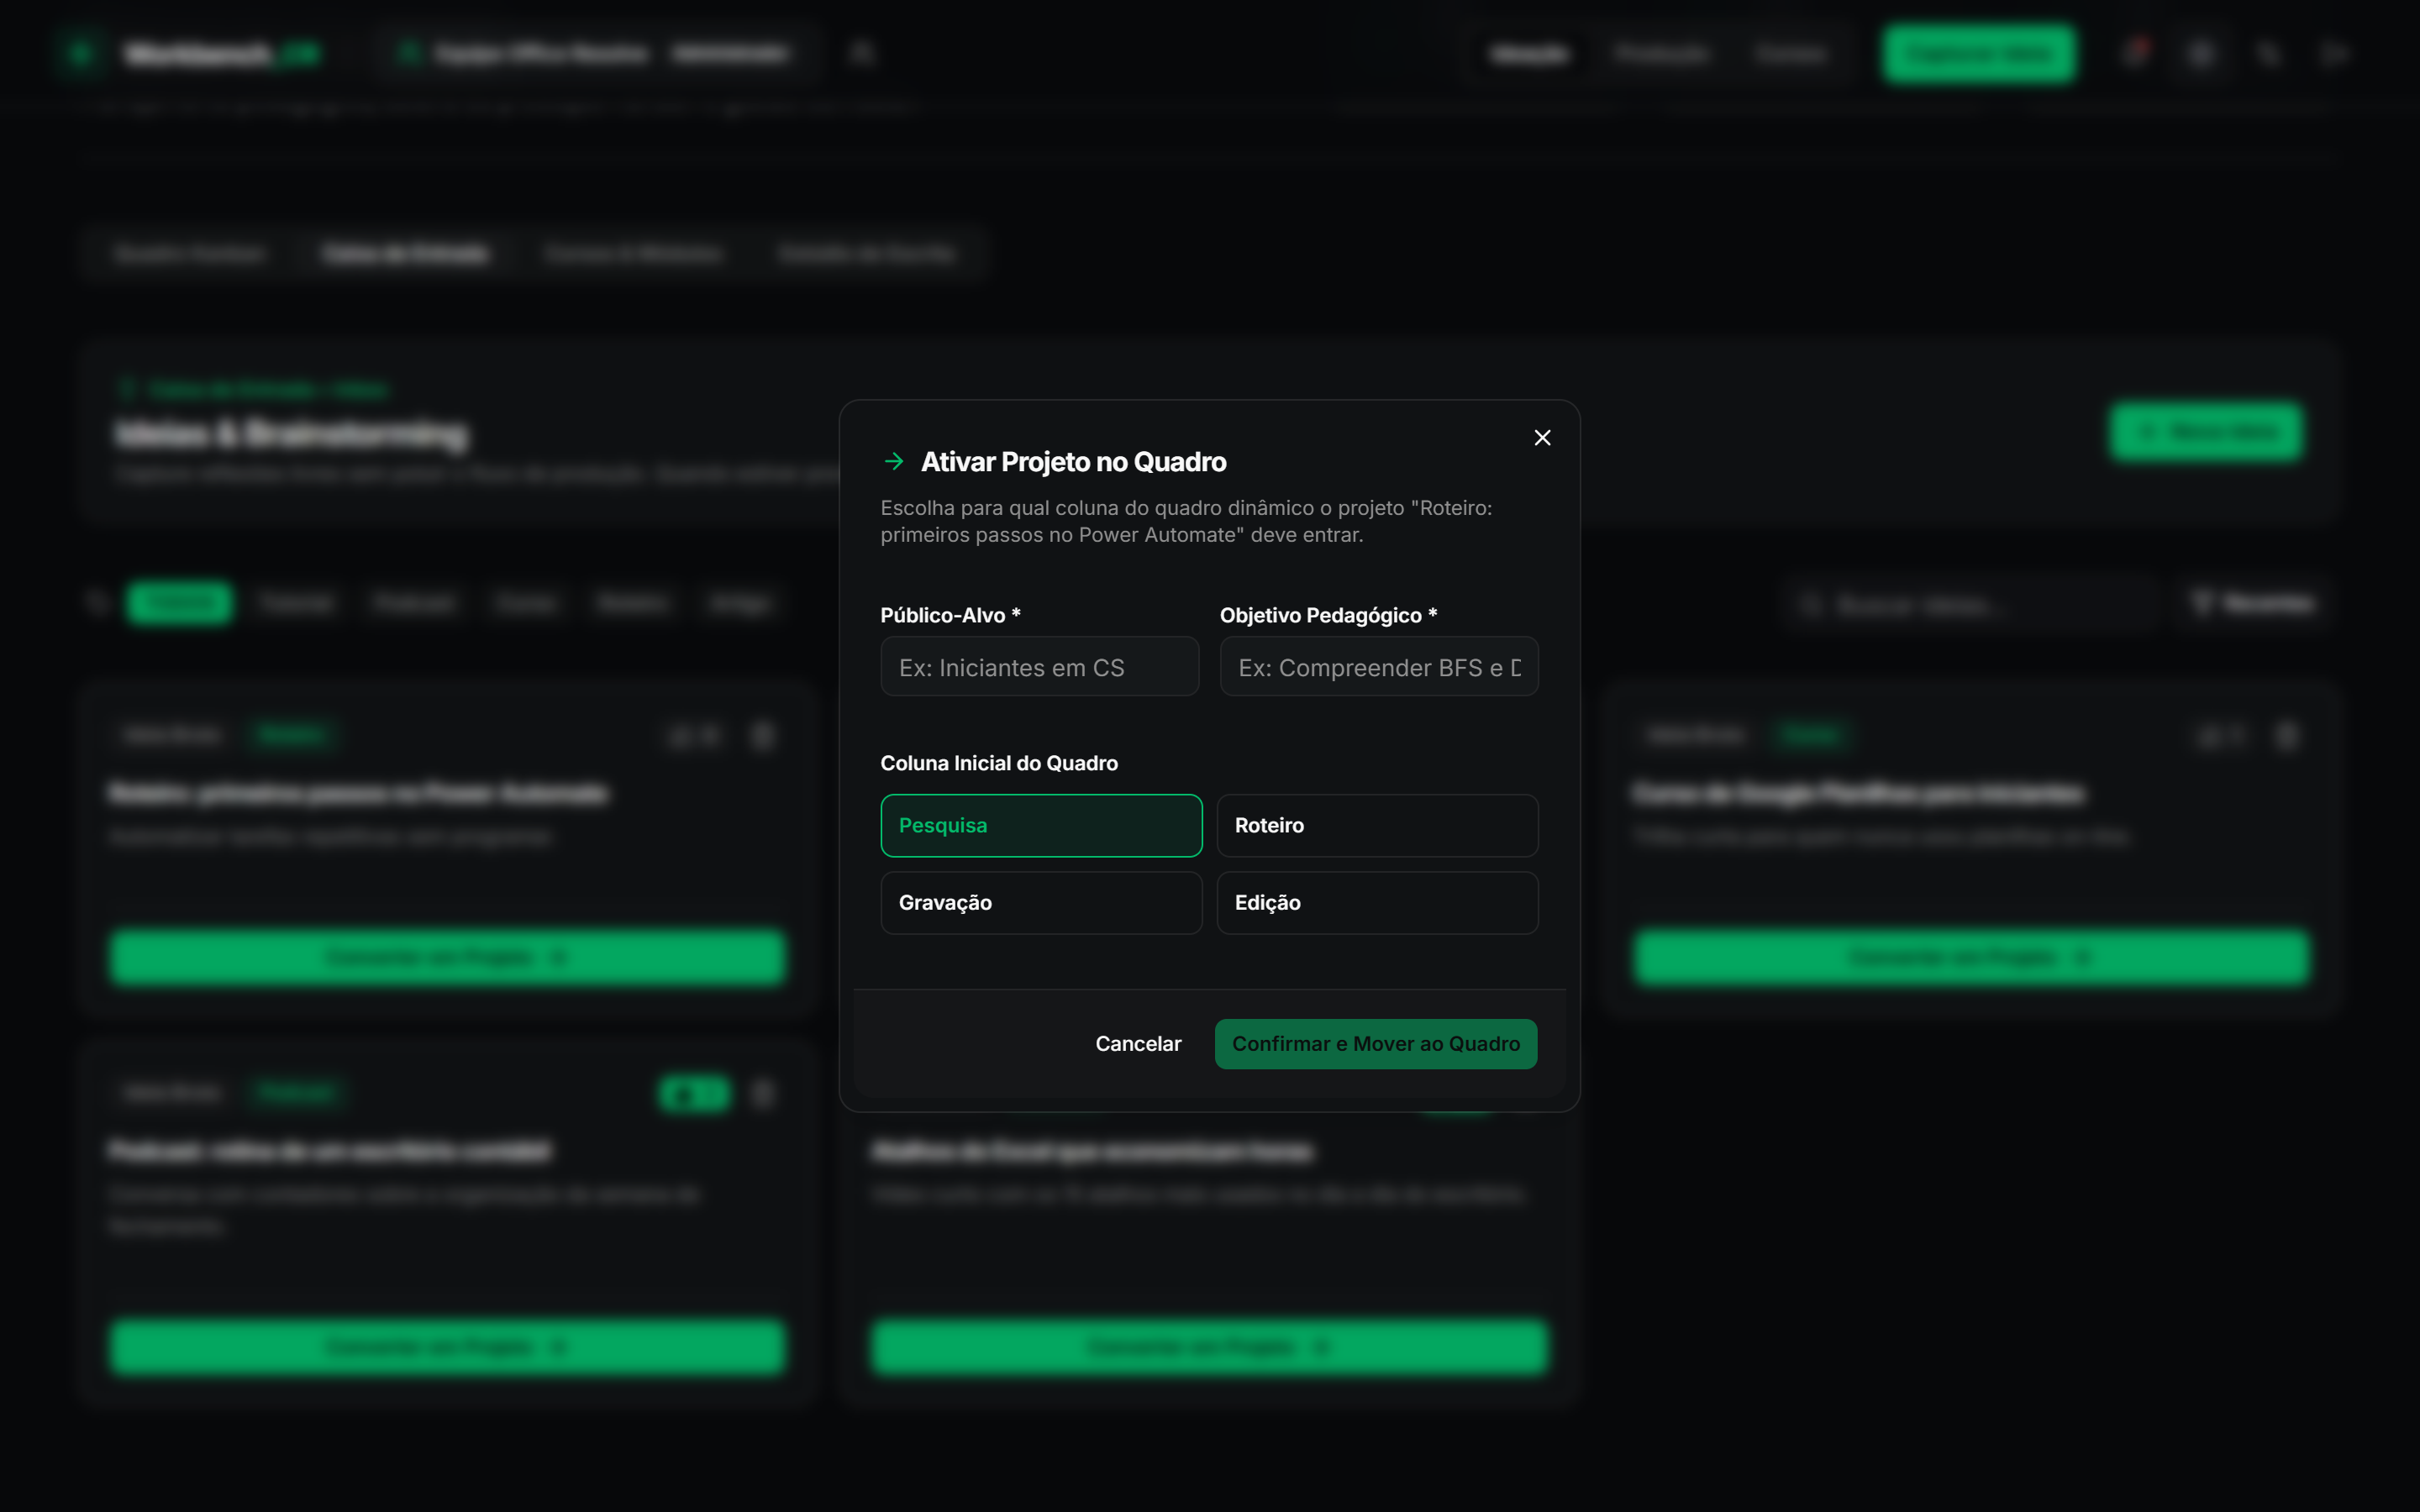
\includegraphics[width=0.85\textwidth]{imagens/09-converter-ideia-em-projeto.png}
    \legend{Fonte: Produzido pelos autores.}
\end{figure}

\section{Detalhes do projeto}

\begin{figure}[H]
    \centering
    \caption{Detalhes do projeto: tarefas, com o progresso calculado pelas tarefas concluídas}
    \label{fig:tela-10}
    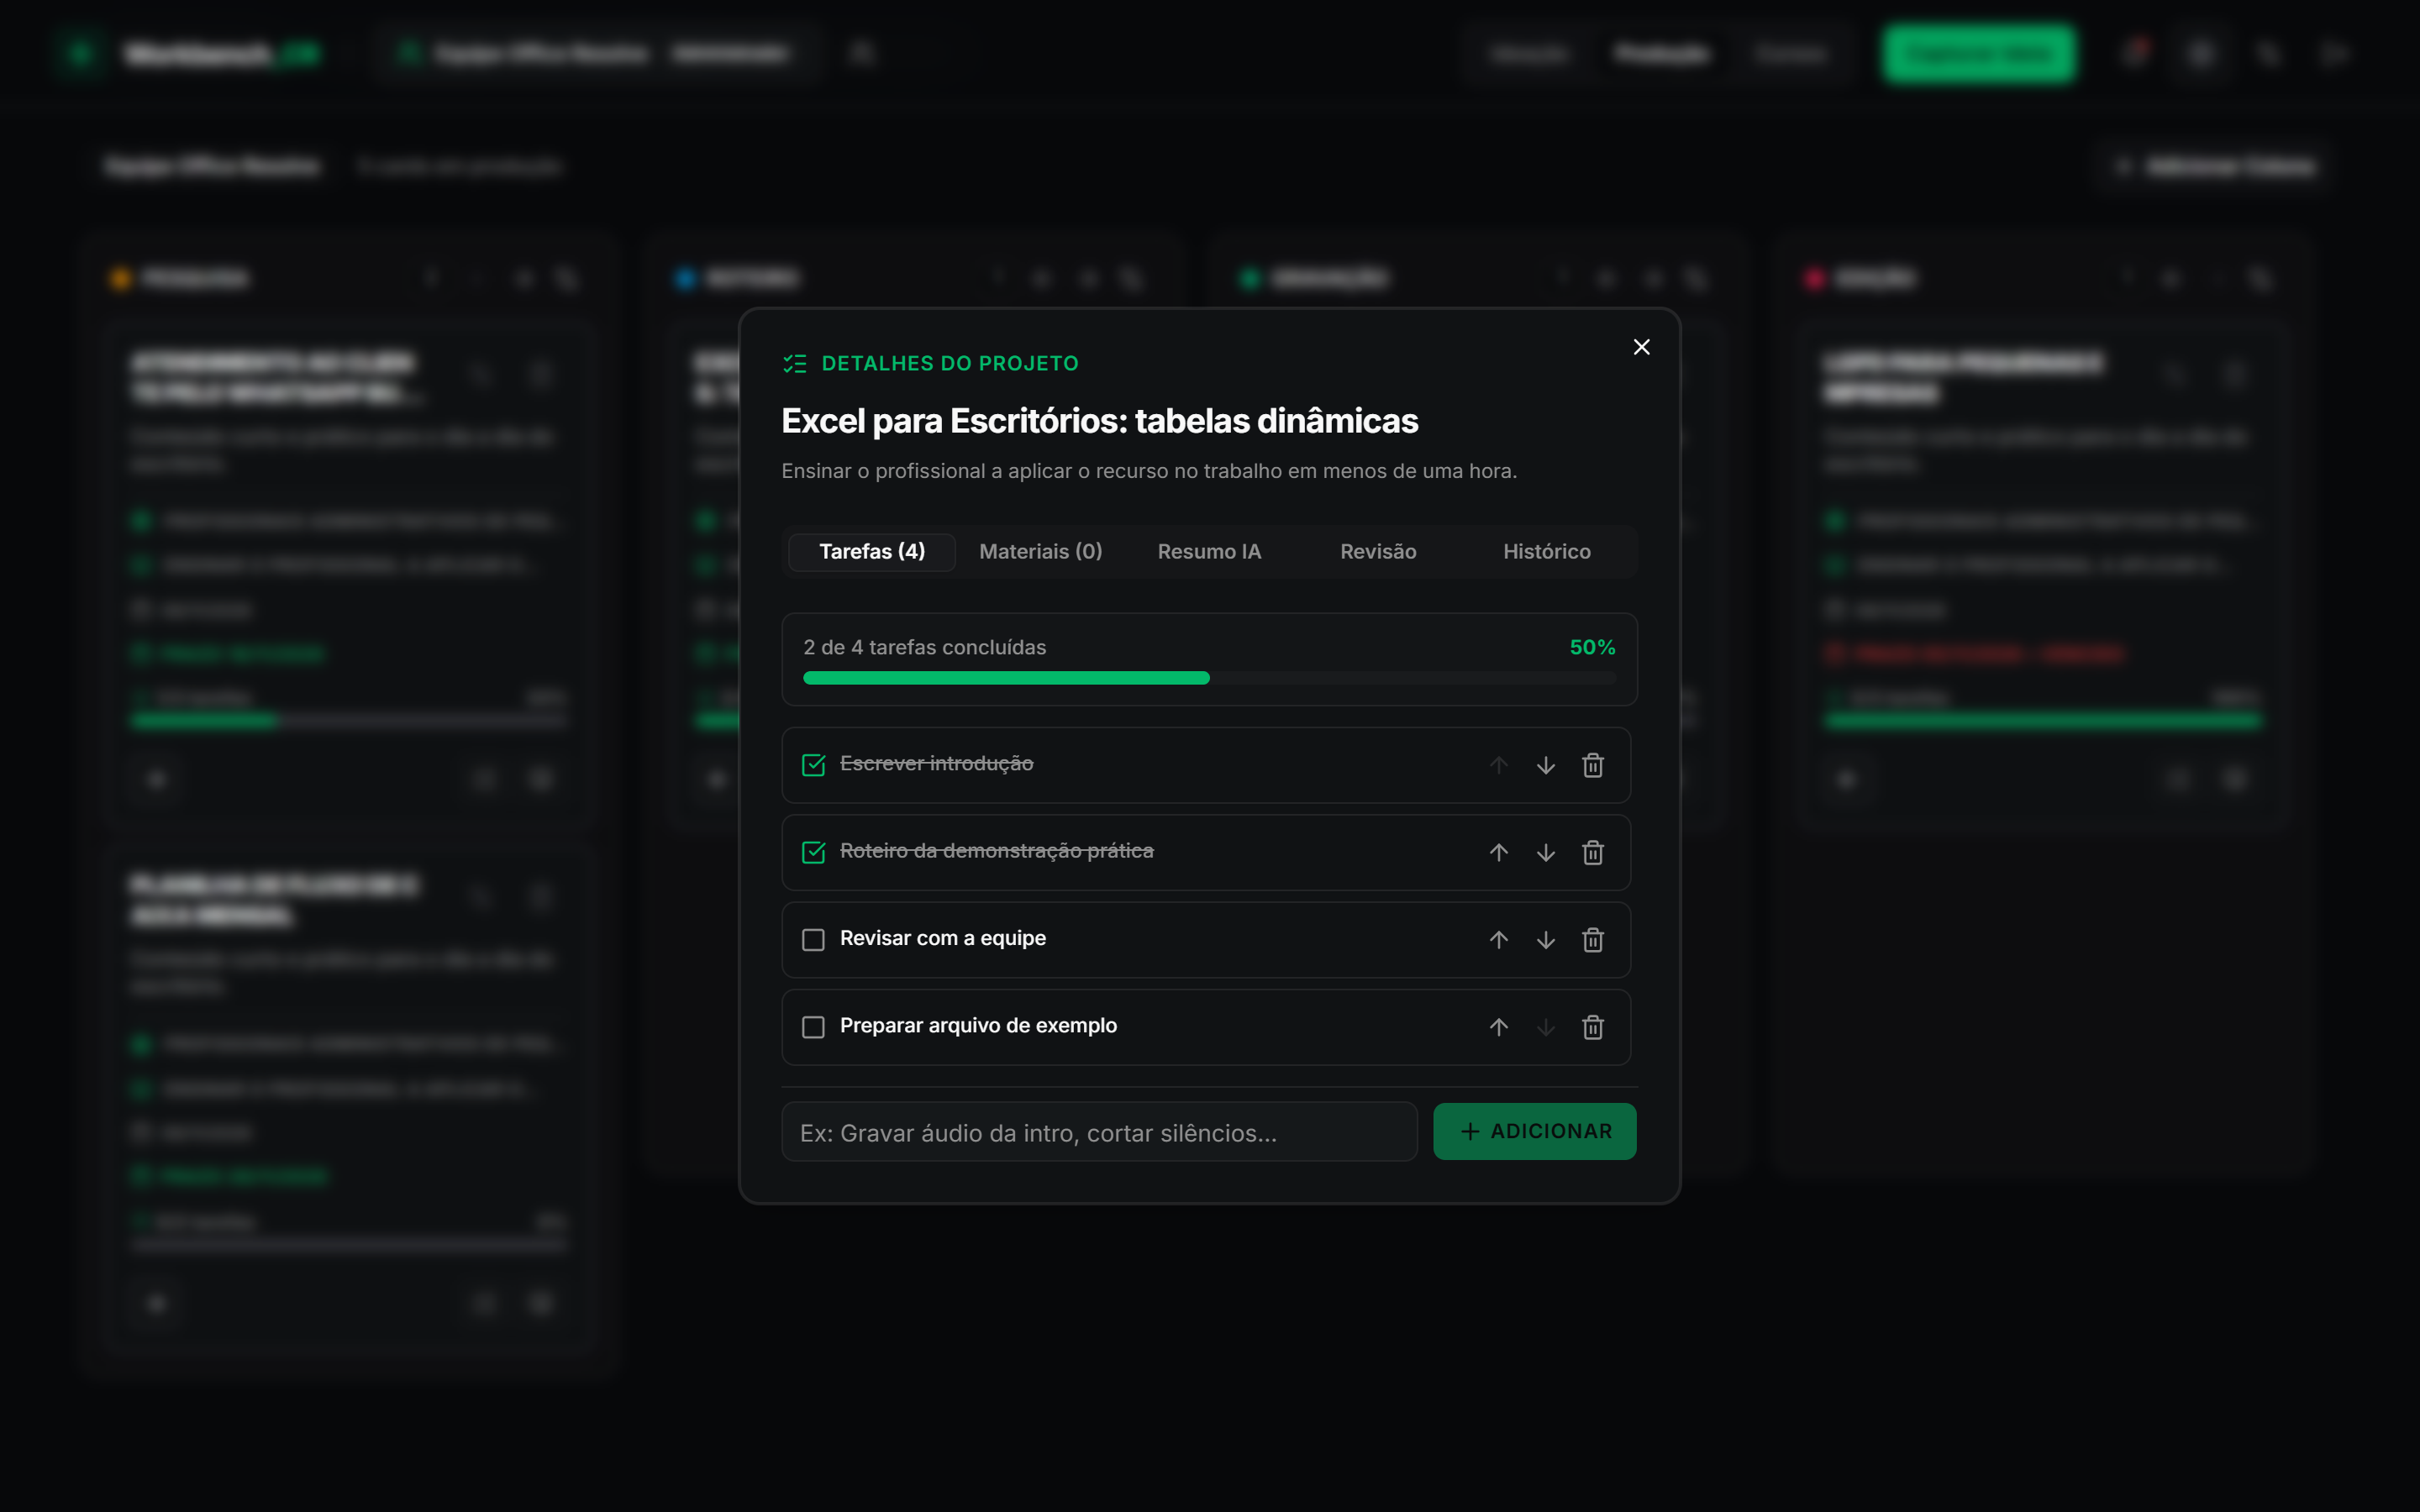
\includegraphics[width=0.85\textwidth]{imagens/10-projeto-tarefas.png}
    \legend{Fonte: Produzido pelos autores.}
\end{figure}

\begin{figure}[H]
    \centering
    \caption{Detalhes do projeto: materiais de apoio, com envio e \textit{download} de arquivos de até 20 MB (RF06)}
    \label{fig:tela-11}
    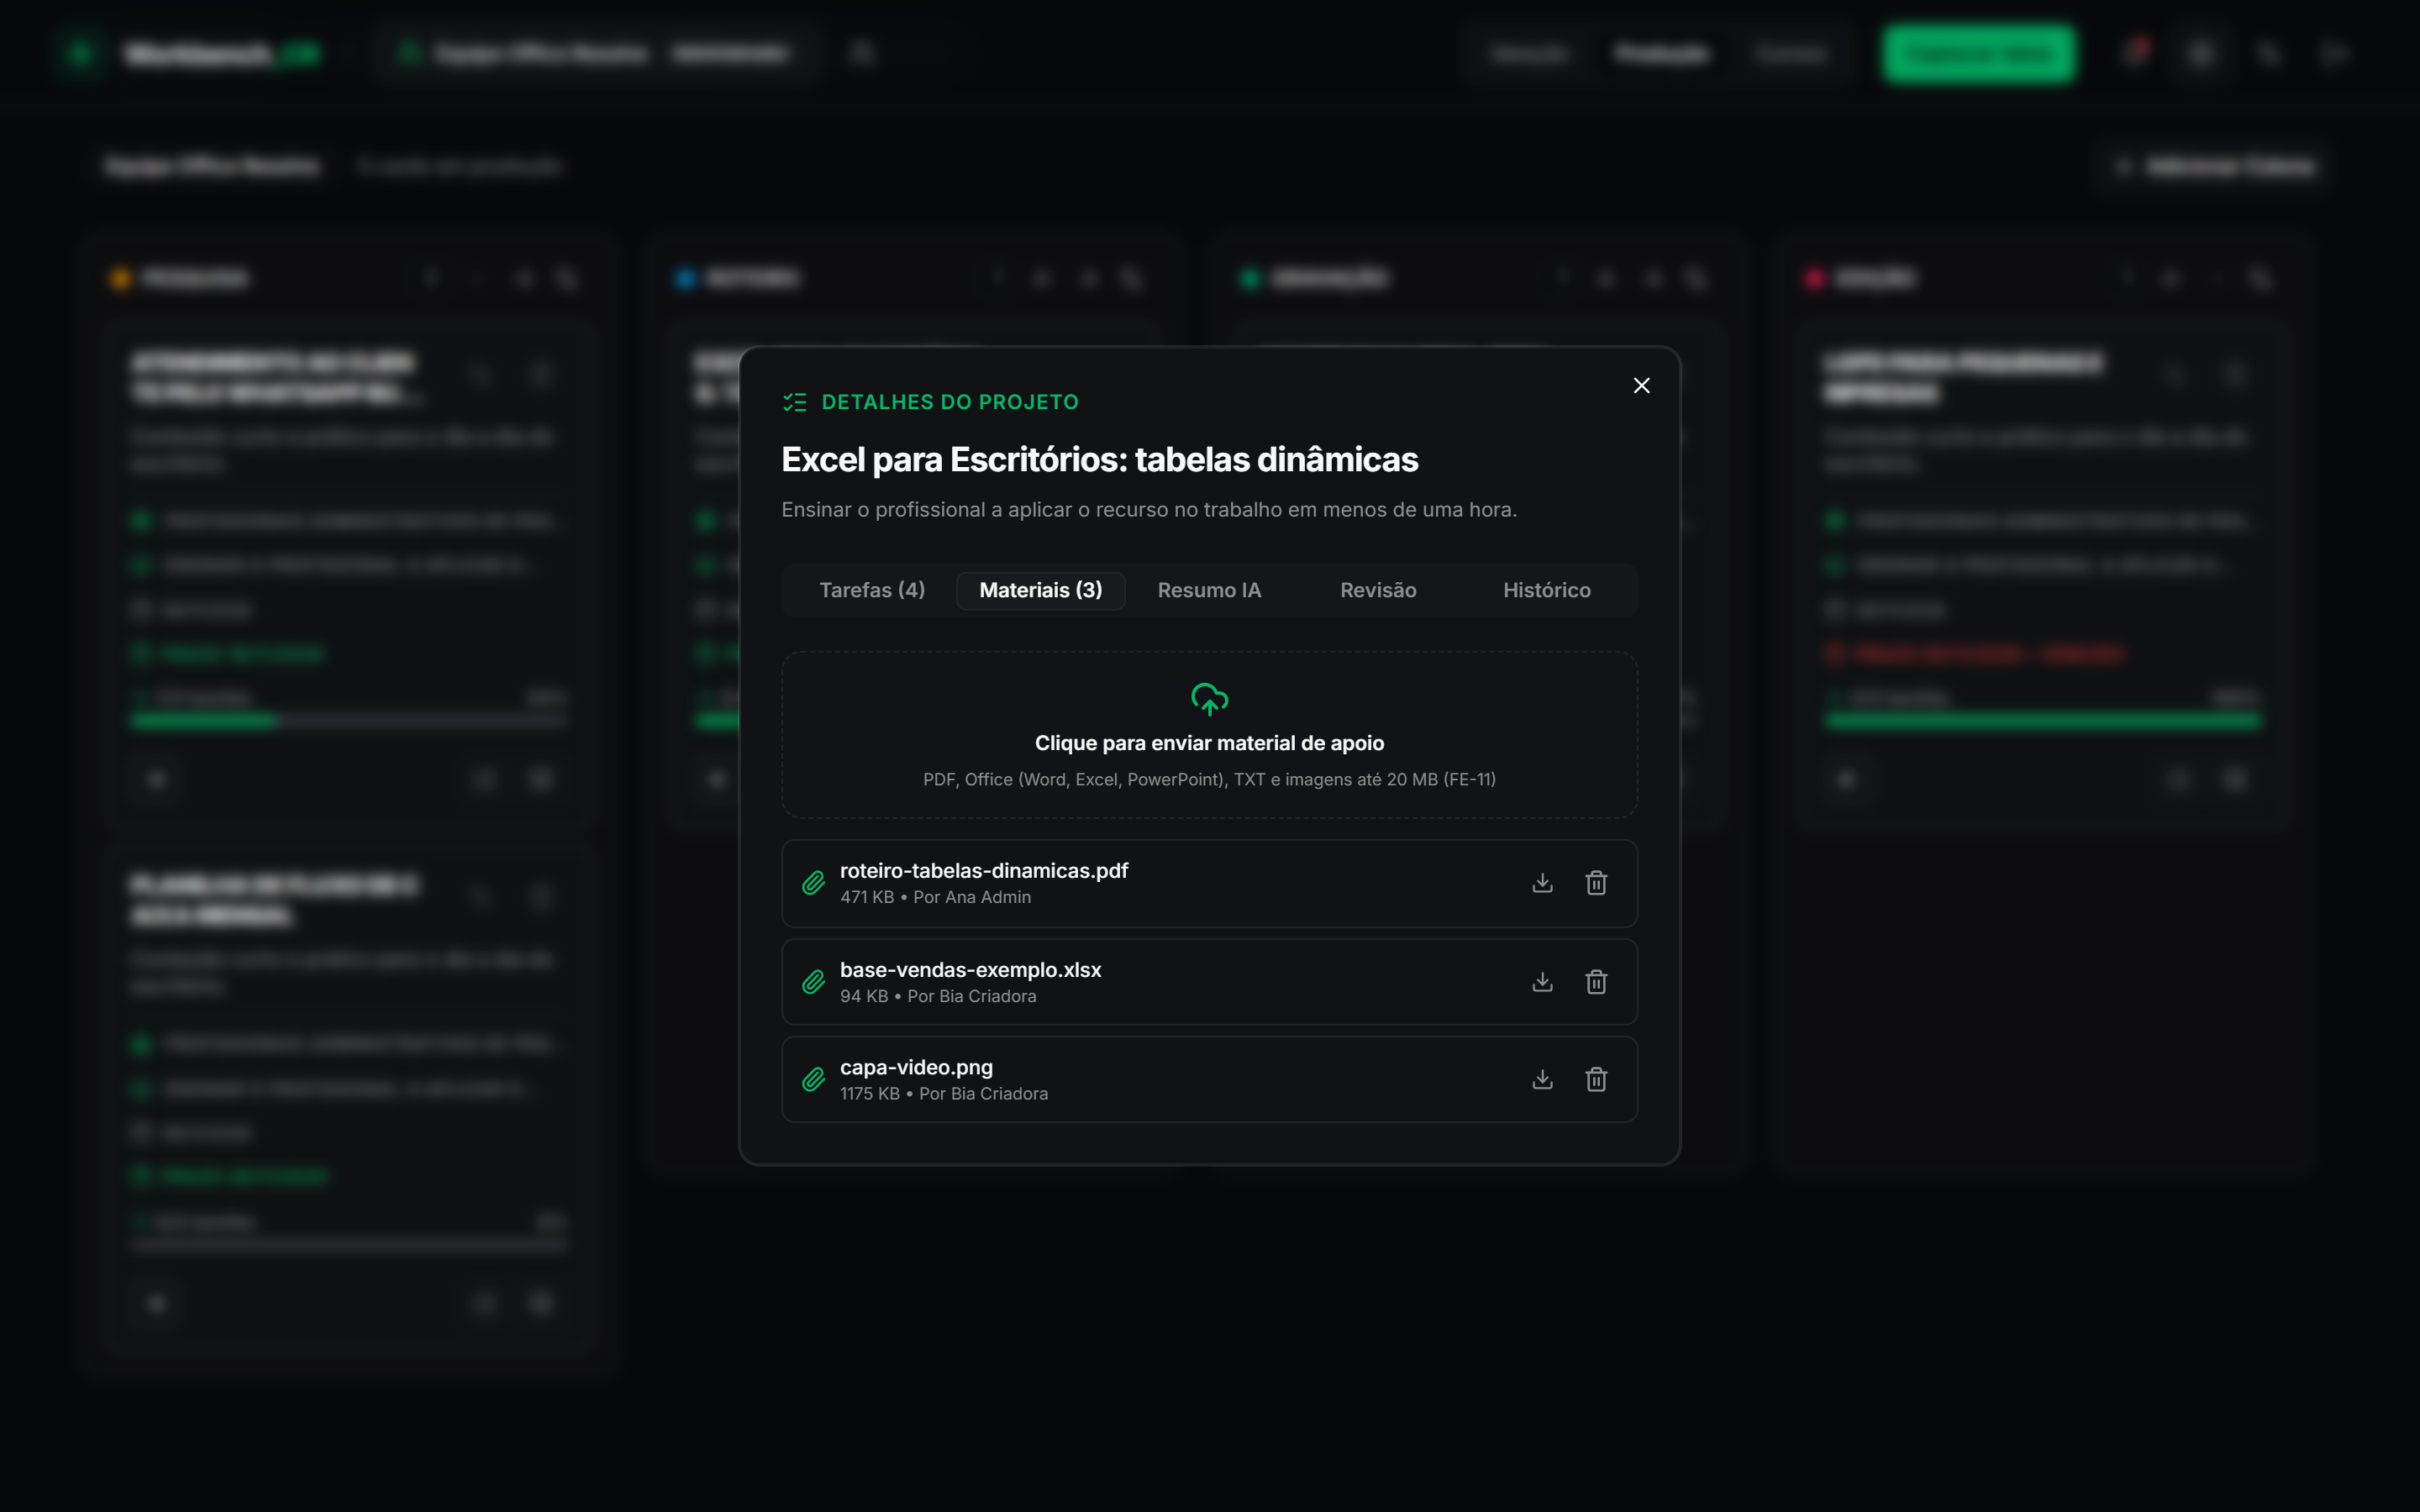
\includegraphics[width=0.85\textwidth]{imagens/11-projeto-materiais.png}
    \legend{Fonte: Produzido pelos autores.}
\end{figure}

\begin{figure}[H]
    \centering
    \caption{Detalhes do projeto: resumo automático gerado pelo serviço de automação a partir do roteiro (RF08)}
    \label{fig:tela-12}
    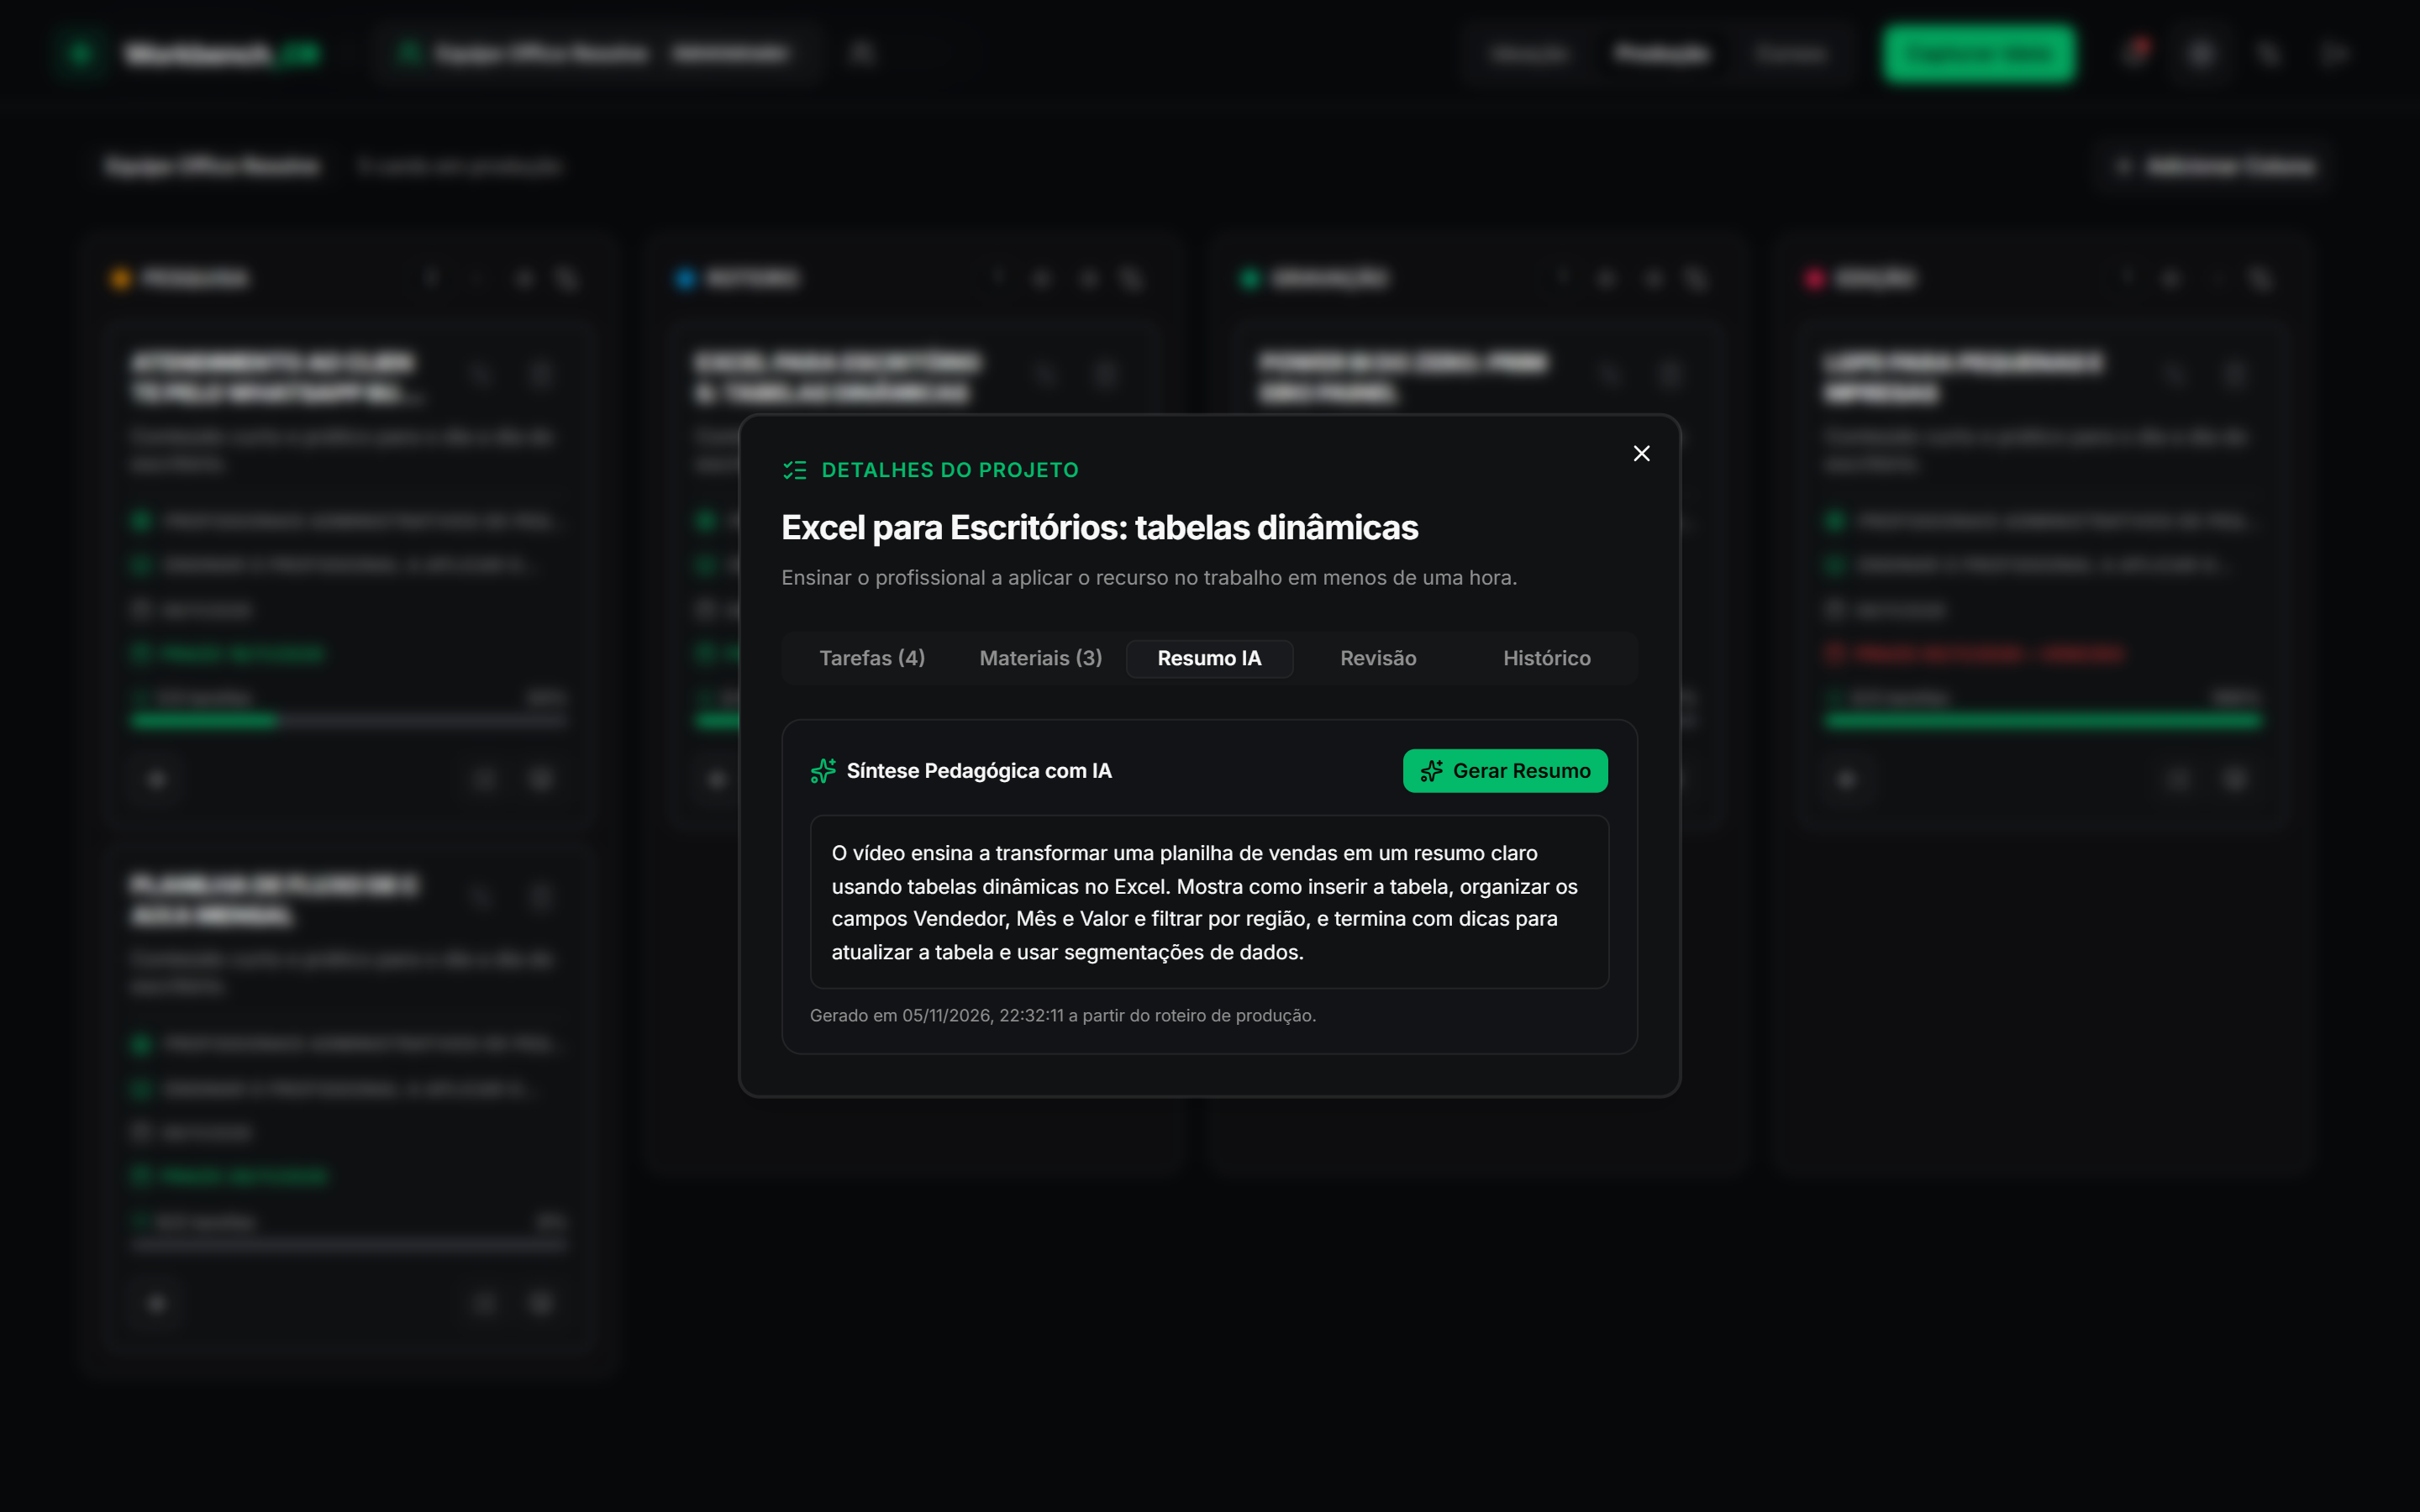
\includegraphics[width=0.85\textwidth]{imagens/12-projeto-resumo-automatico.png}
    \legend{Fonte: Produzido pelos autores.}
\end{figure}

\begin{figure}[H]
    \centering
    \caption{Detalhes do projeto: revisão, em que o revisor aprova o projeto ou pede alterações}
    \label{fig:tela-13}
    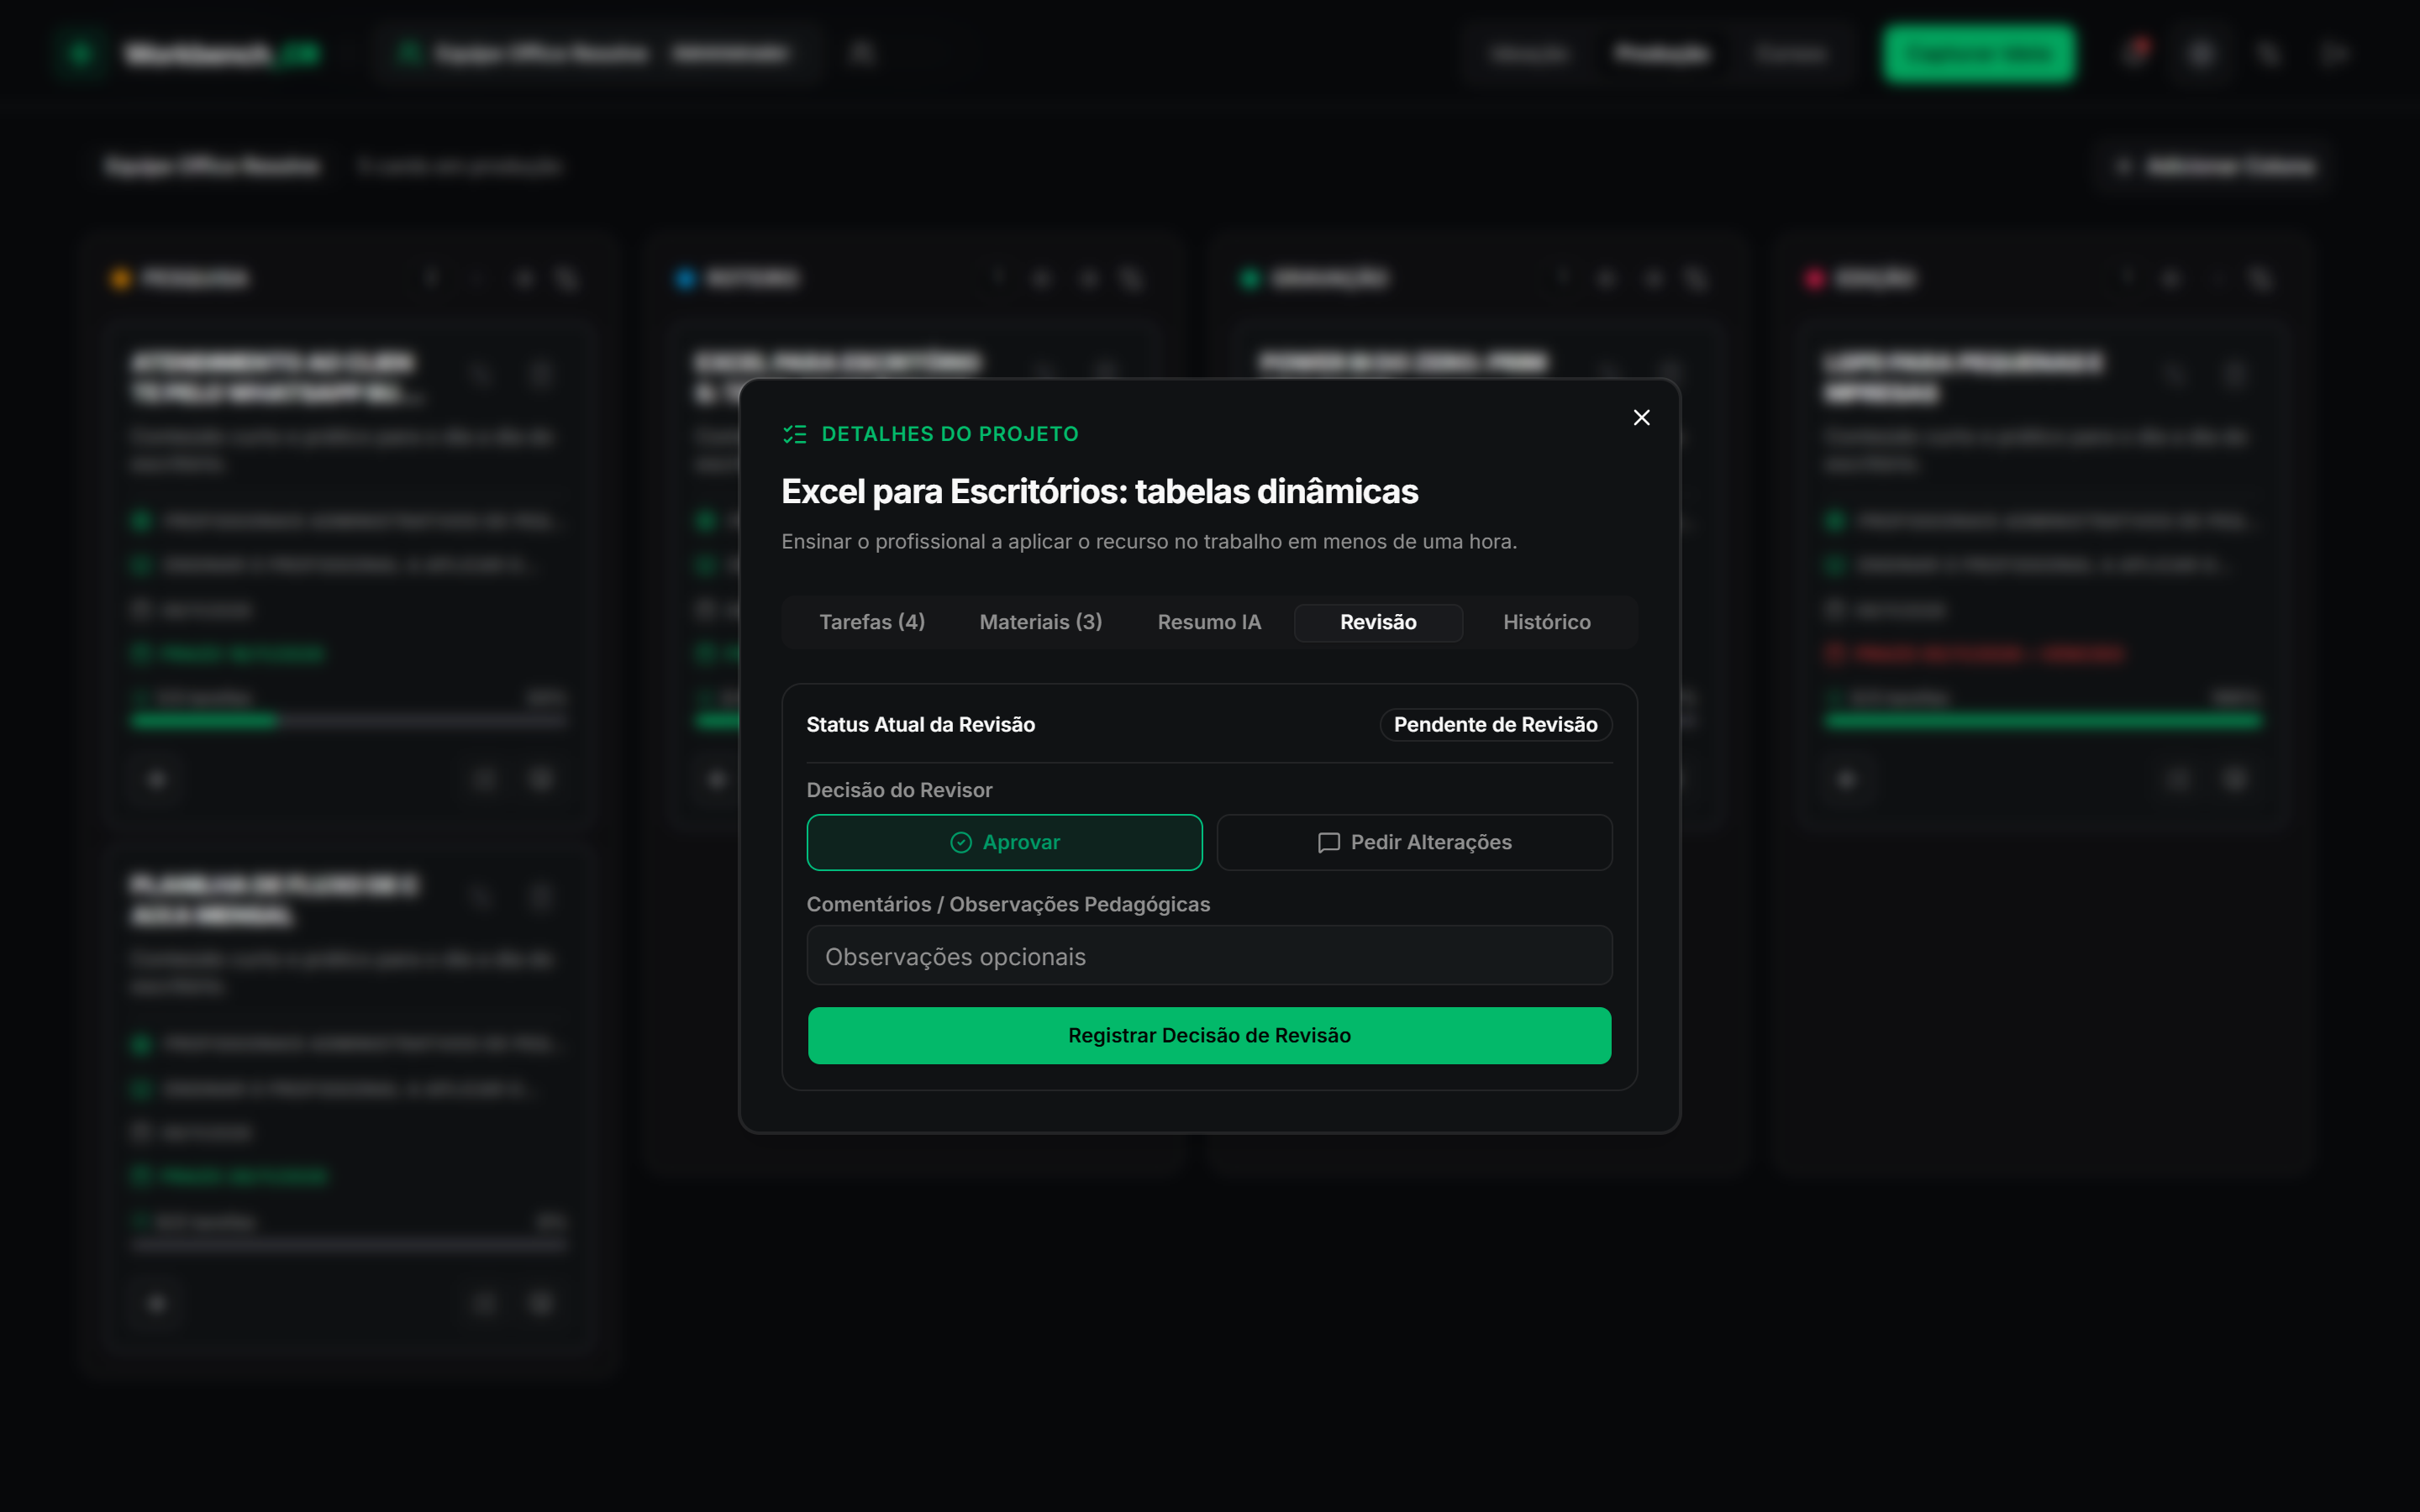
\includegraphics[width=0.85\textwidth]{imagens/13-projeto-revisao.png}
    \legend{Fonte: Produzido pelos autores.}
\end{figure}

\begin{figure}[H]
    \centering
    \caption{Detalhes do projeto: histórico das mudanças de coluna, com a data e quem fez cada mudança}
    \label{fig:tela-14}
    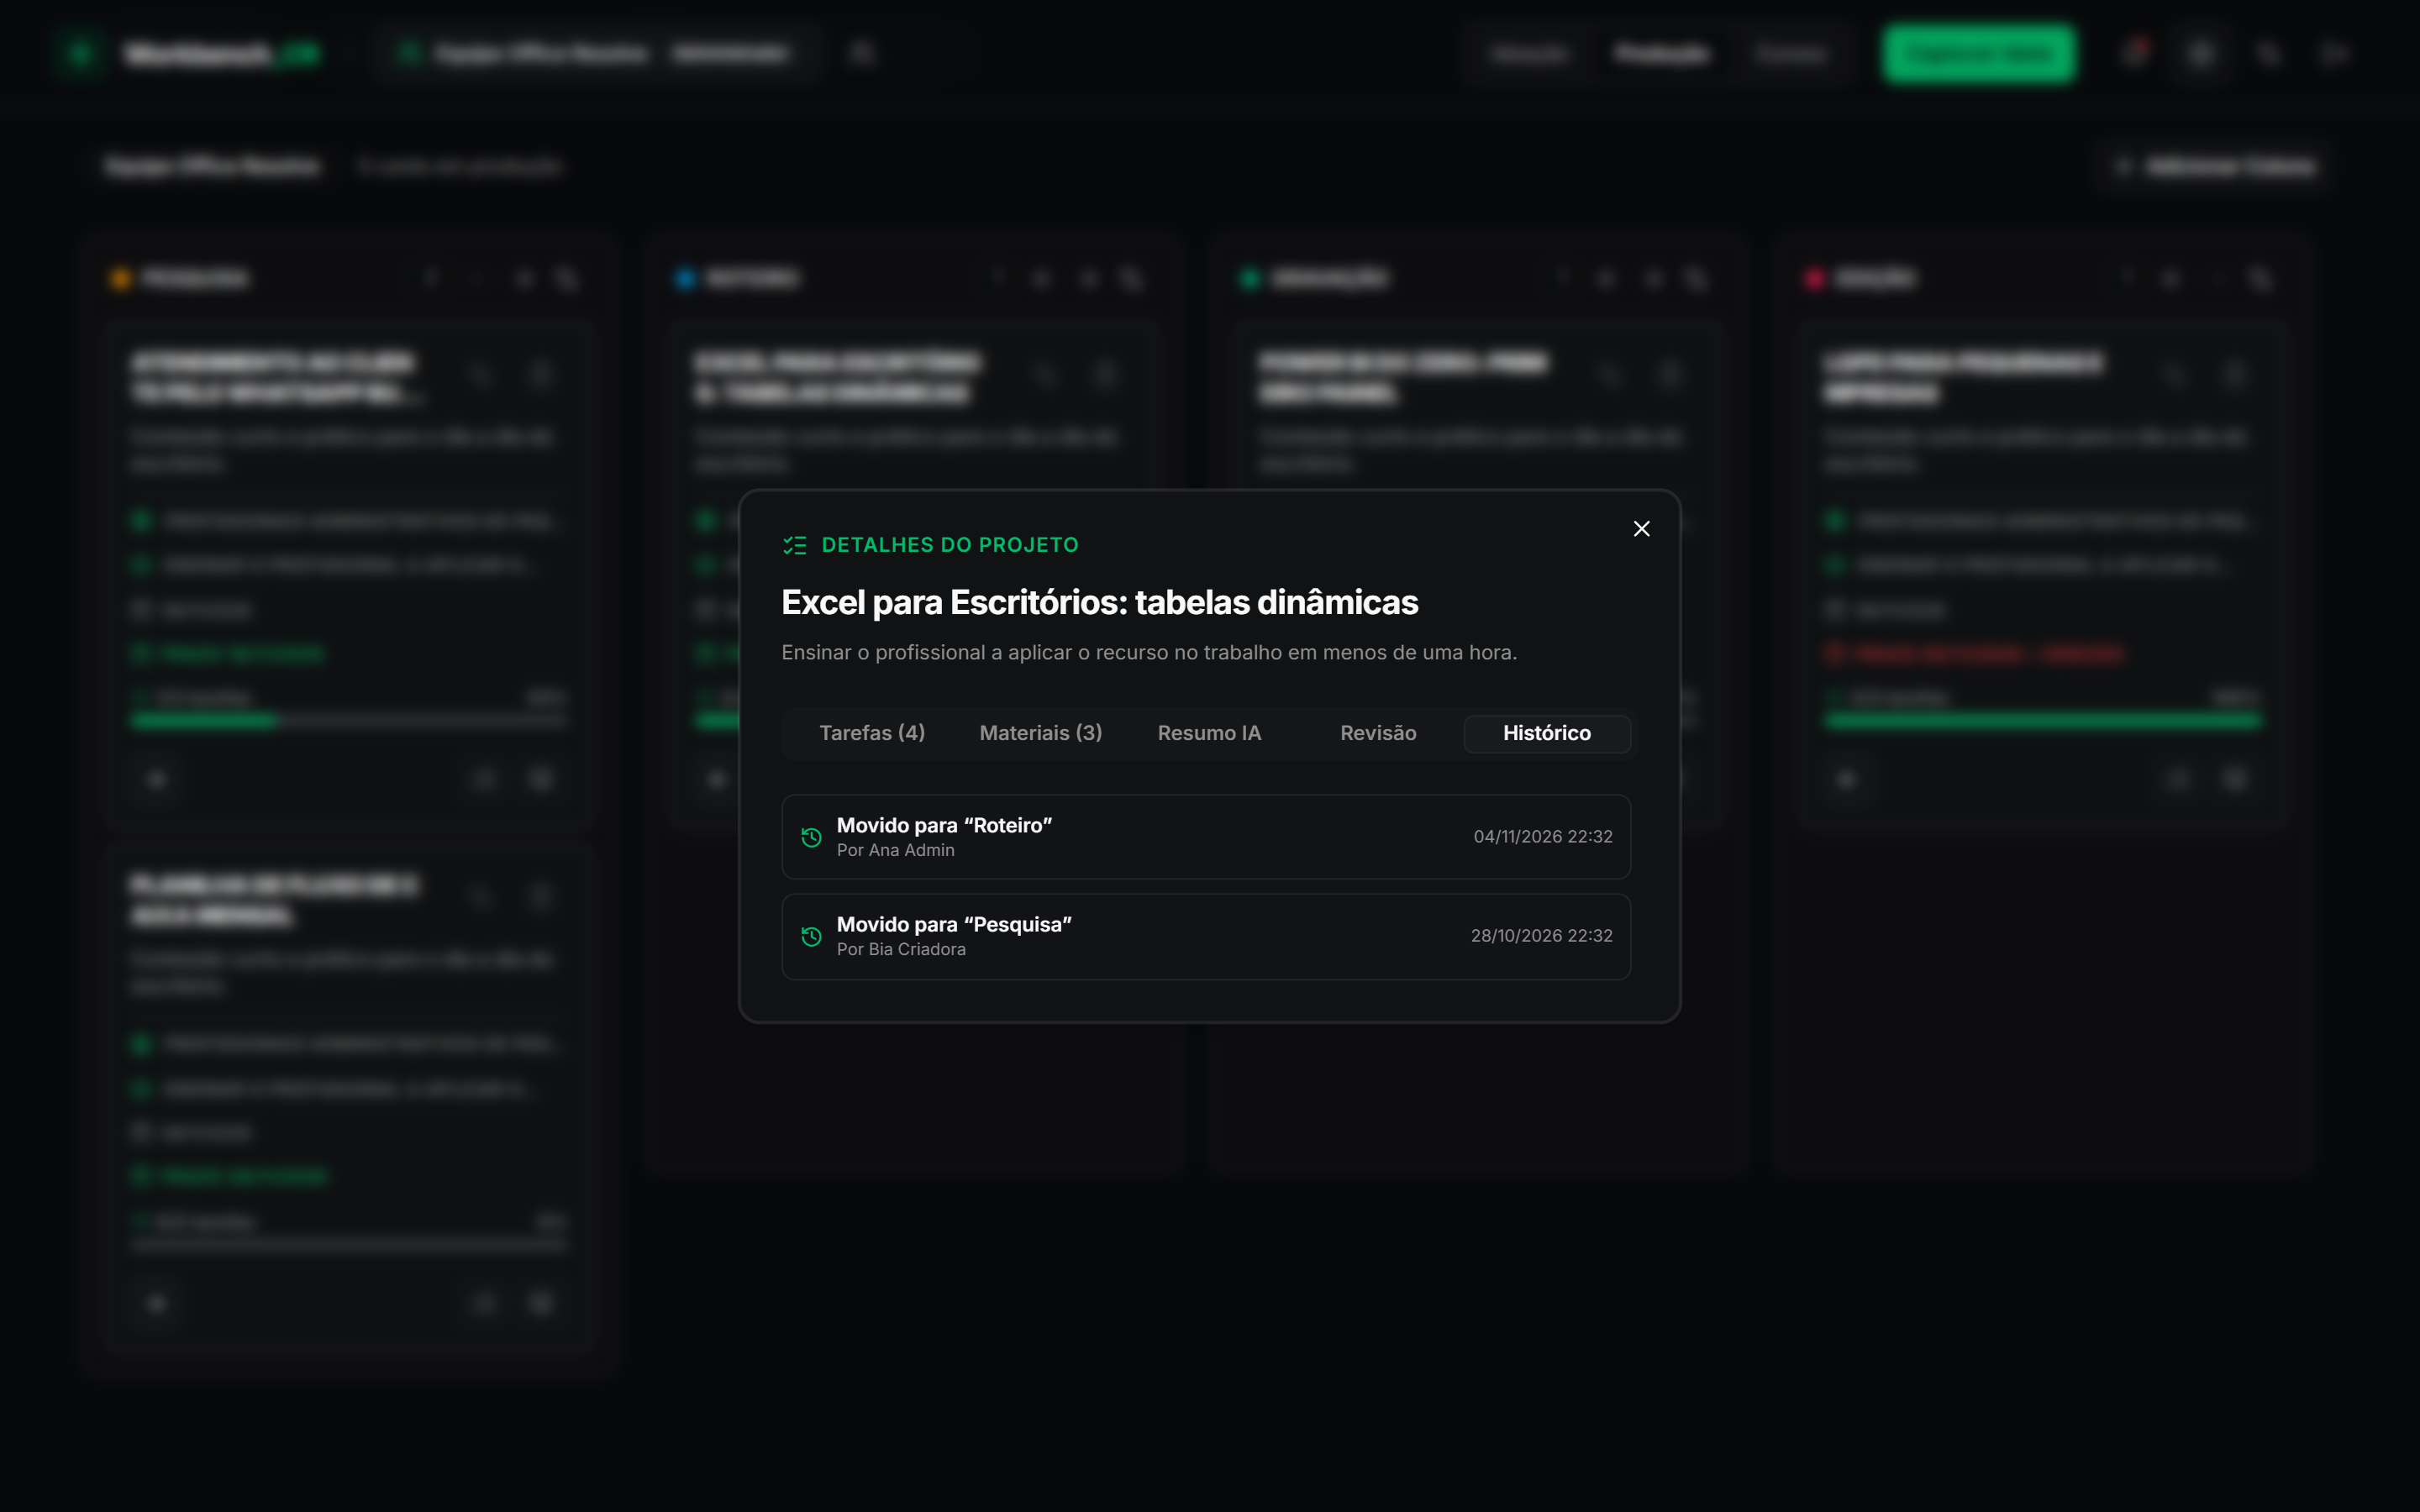
\includegraphics[width=0.85\textwidth]{imagens/14-projeto-historico.png}
    \legend{Fonte: Produzido pelos autores.}
\end{figure}

\section{Roteiro}

\begin{figure}[H]
    \centering
    \caption{Estúdio de Escrita, com o editor de roteiro, formatação, versões, exportação em Markdown e impressão (RF07)}
    \label{fig:tela-15}
    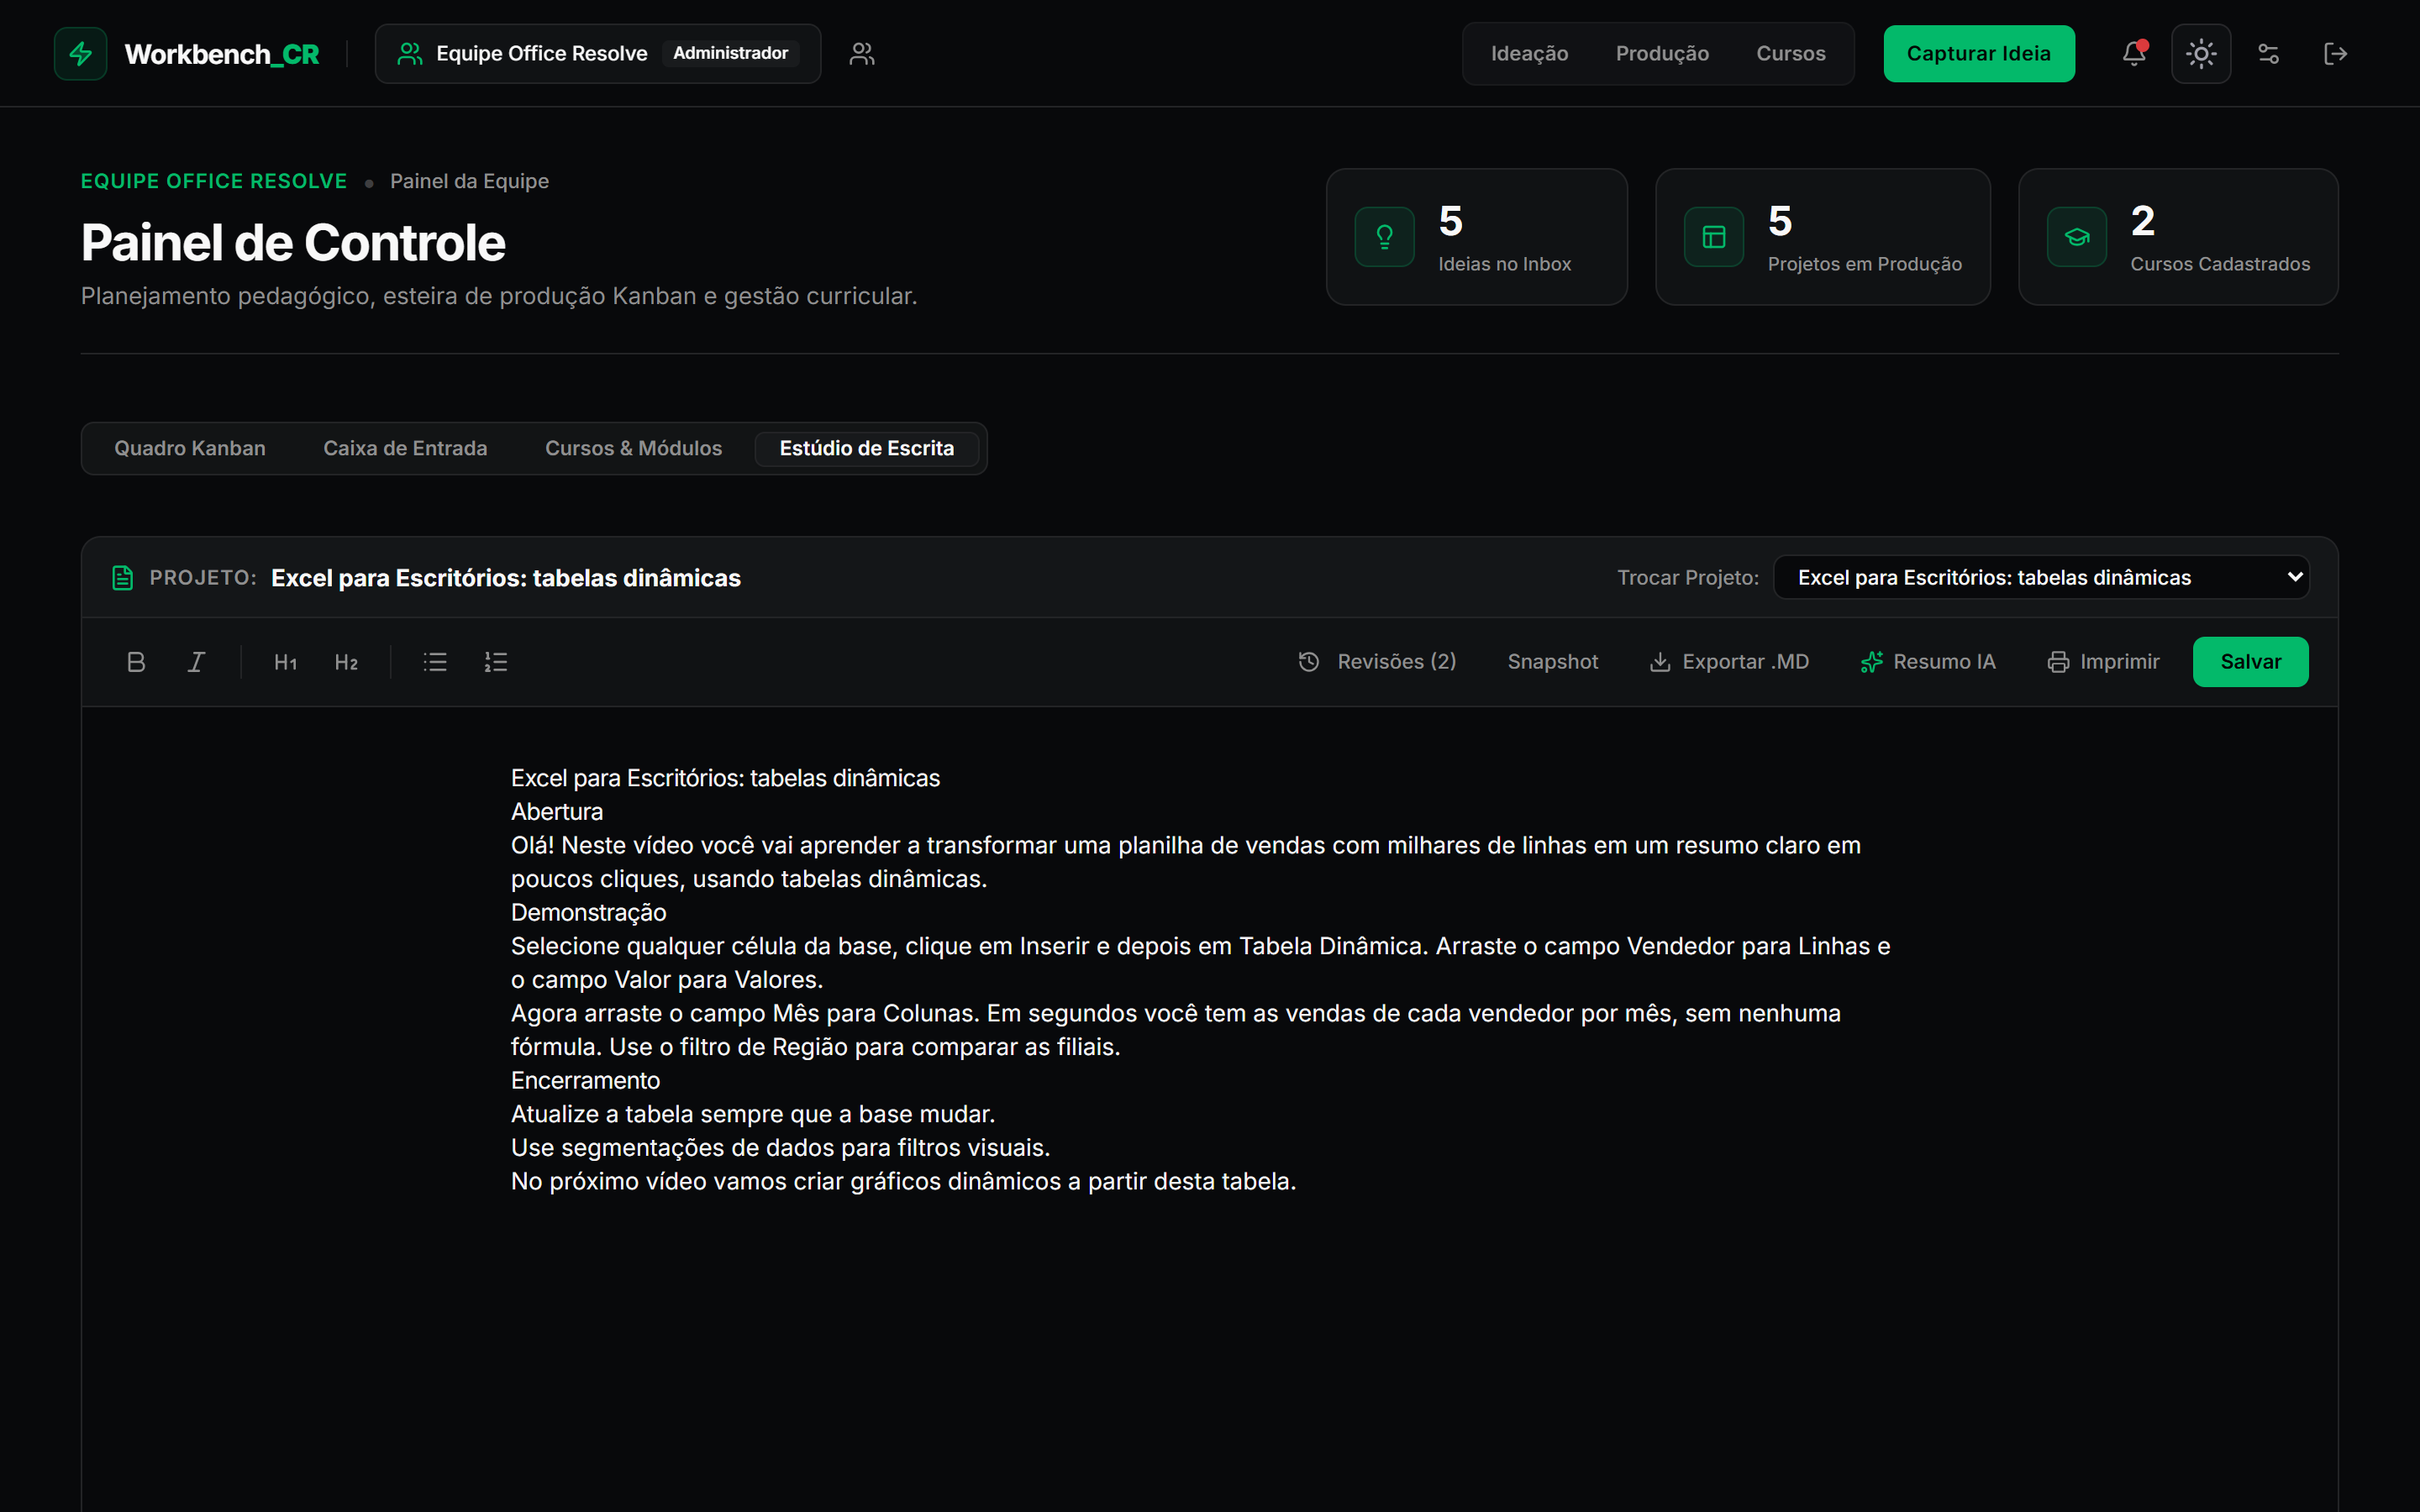
\includegraphics[width=0.85\textwidth]{imagens/15-estudio-de-escrita.png}
    \legend{Fonte: Produzido pelos autores.}
\end{figure}

\begin{figure}[H]
    \centering
    \caption{Histórico de versões do roteiro, que podem ser consultadas e restauradas (RN02)}
    \label{fig:tela-16}
    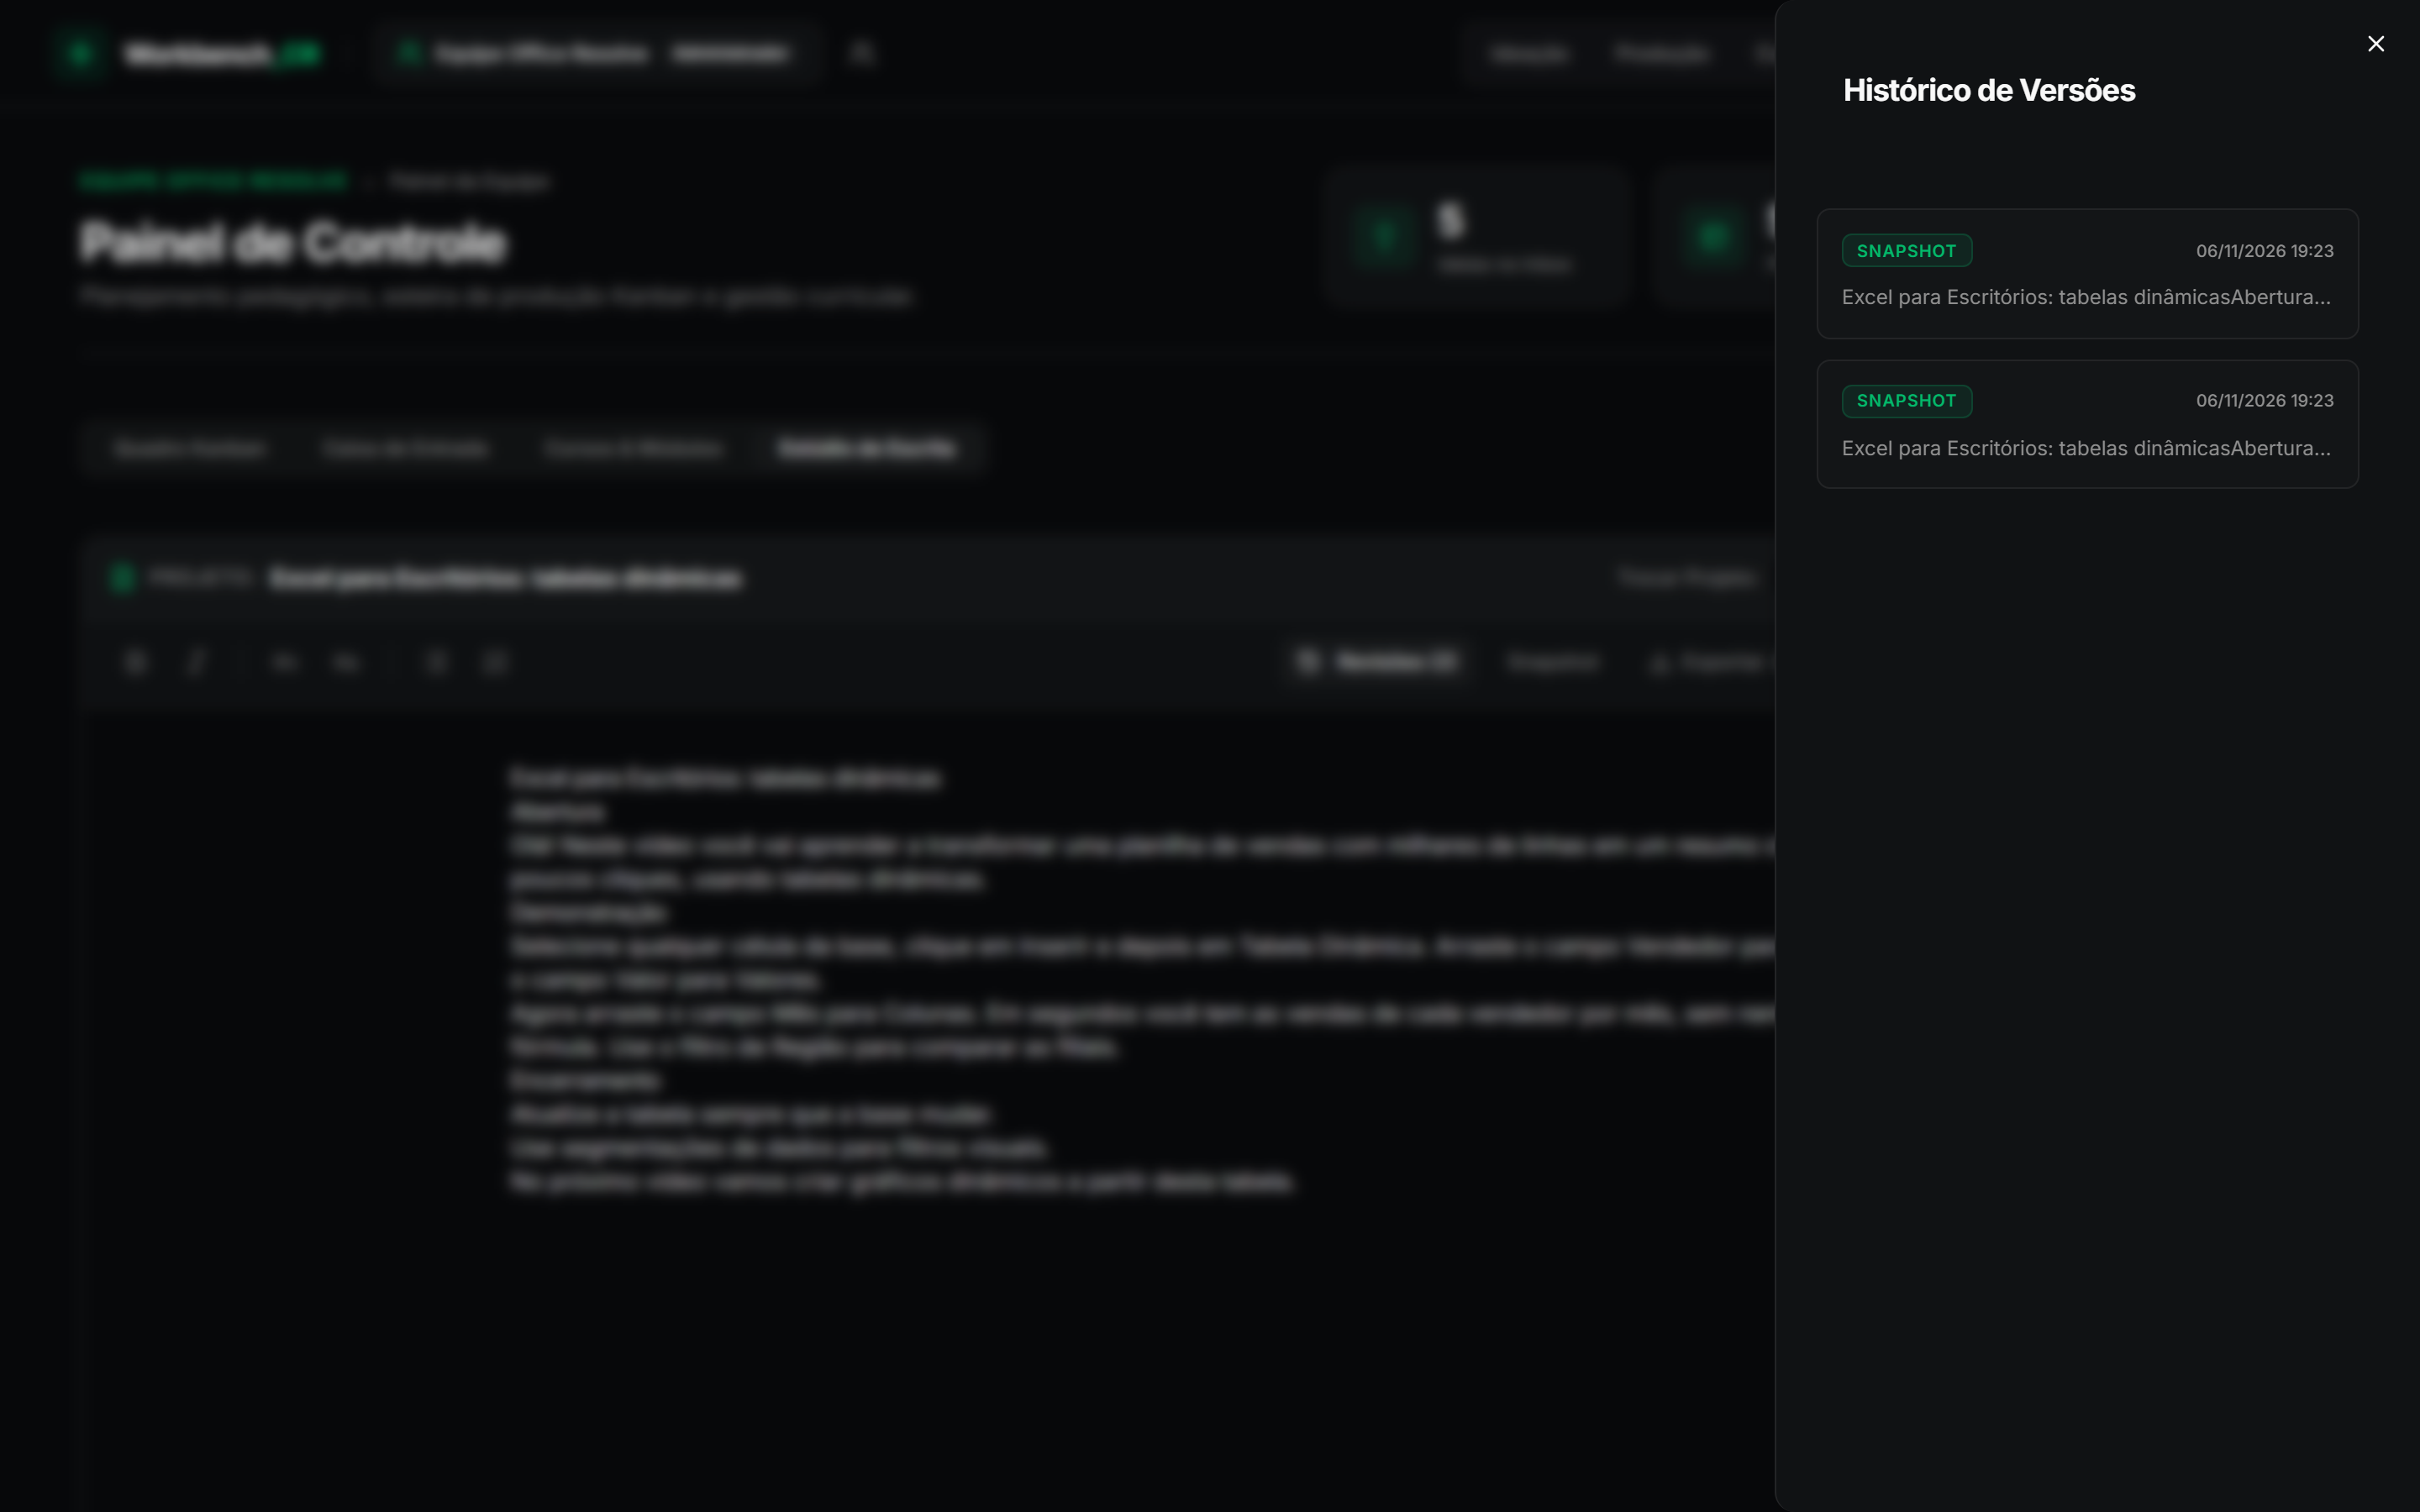
\includegraphics[width=0.85\textwidth]{imagens/16-versoes-do-roteiro.png}
    \legend{Fonte: Produzido pelos autores.}
\end{figure}

\section{Cursos}

\begin{figure}[H]
    \centering
    \caption{Lista de cursos da equipe}
    \label{fig:tela-17}
    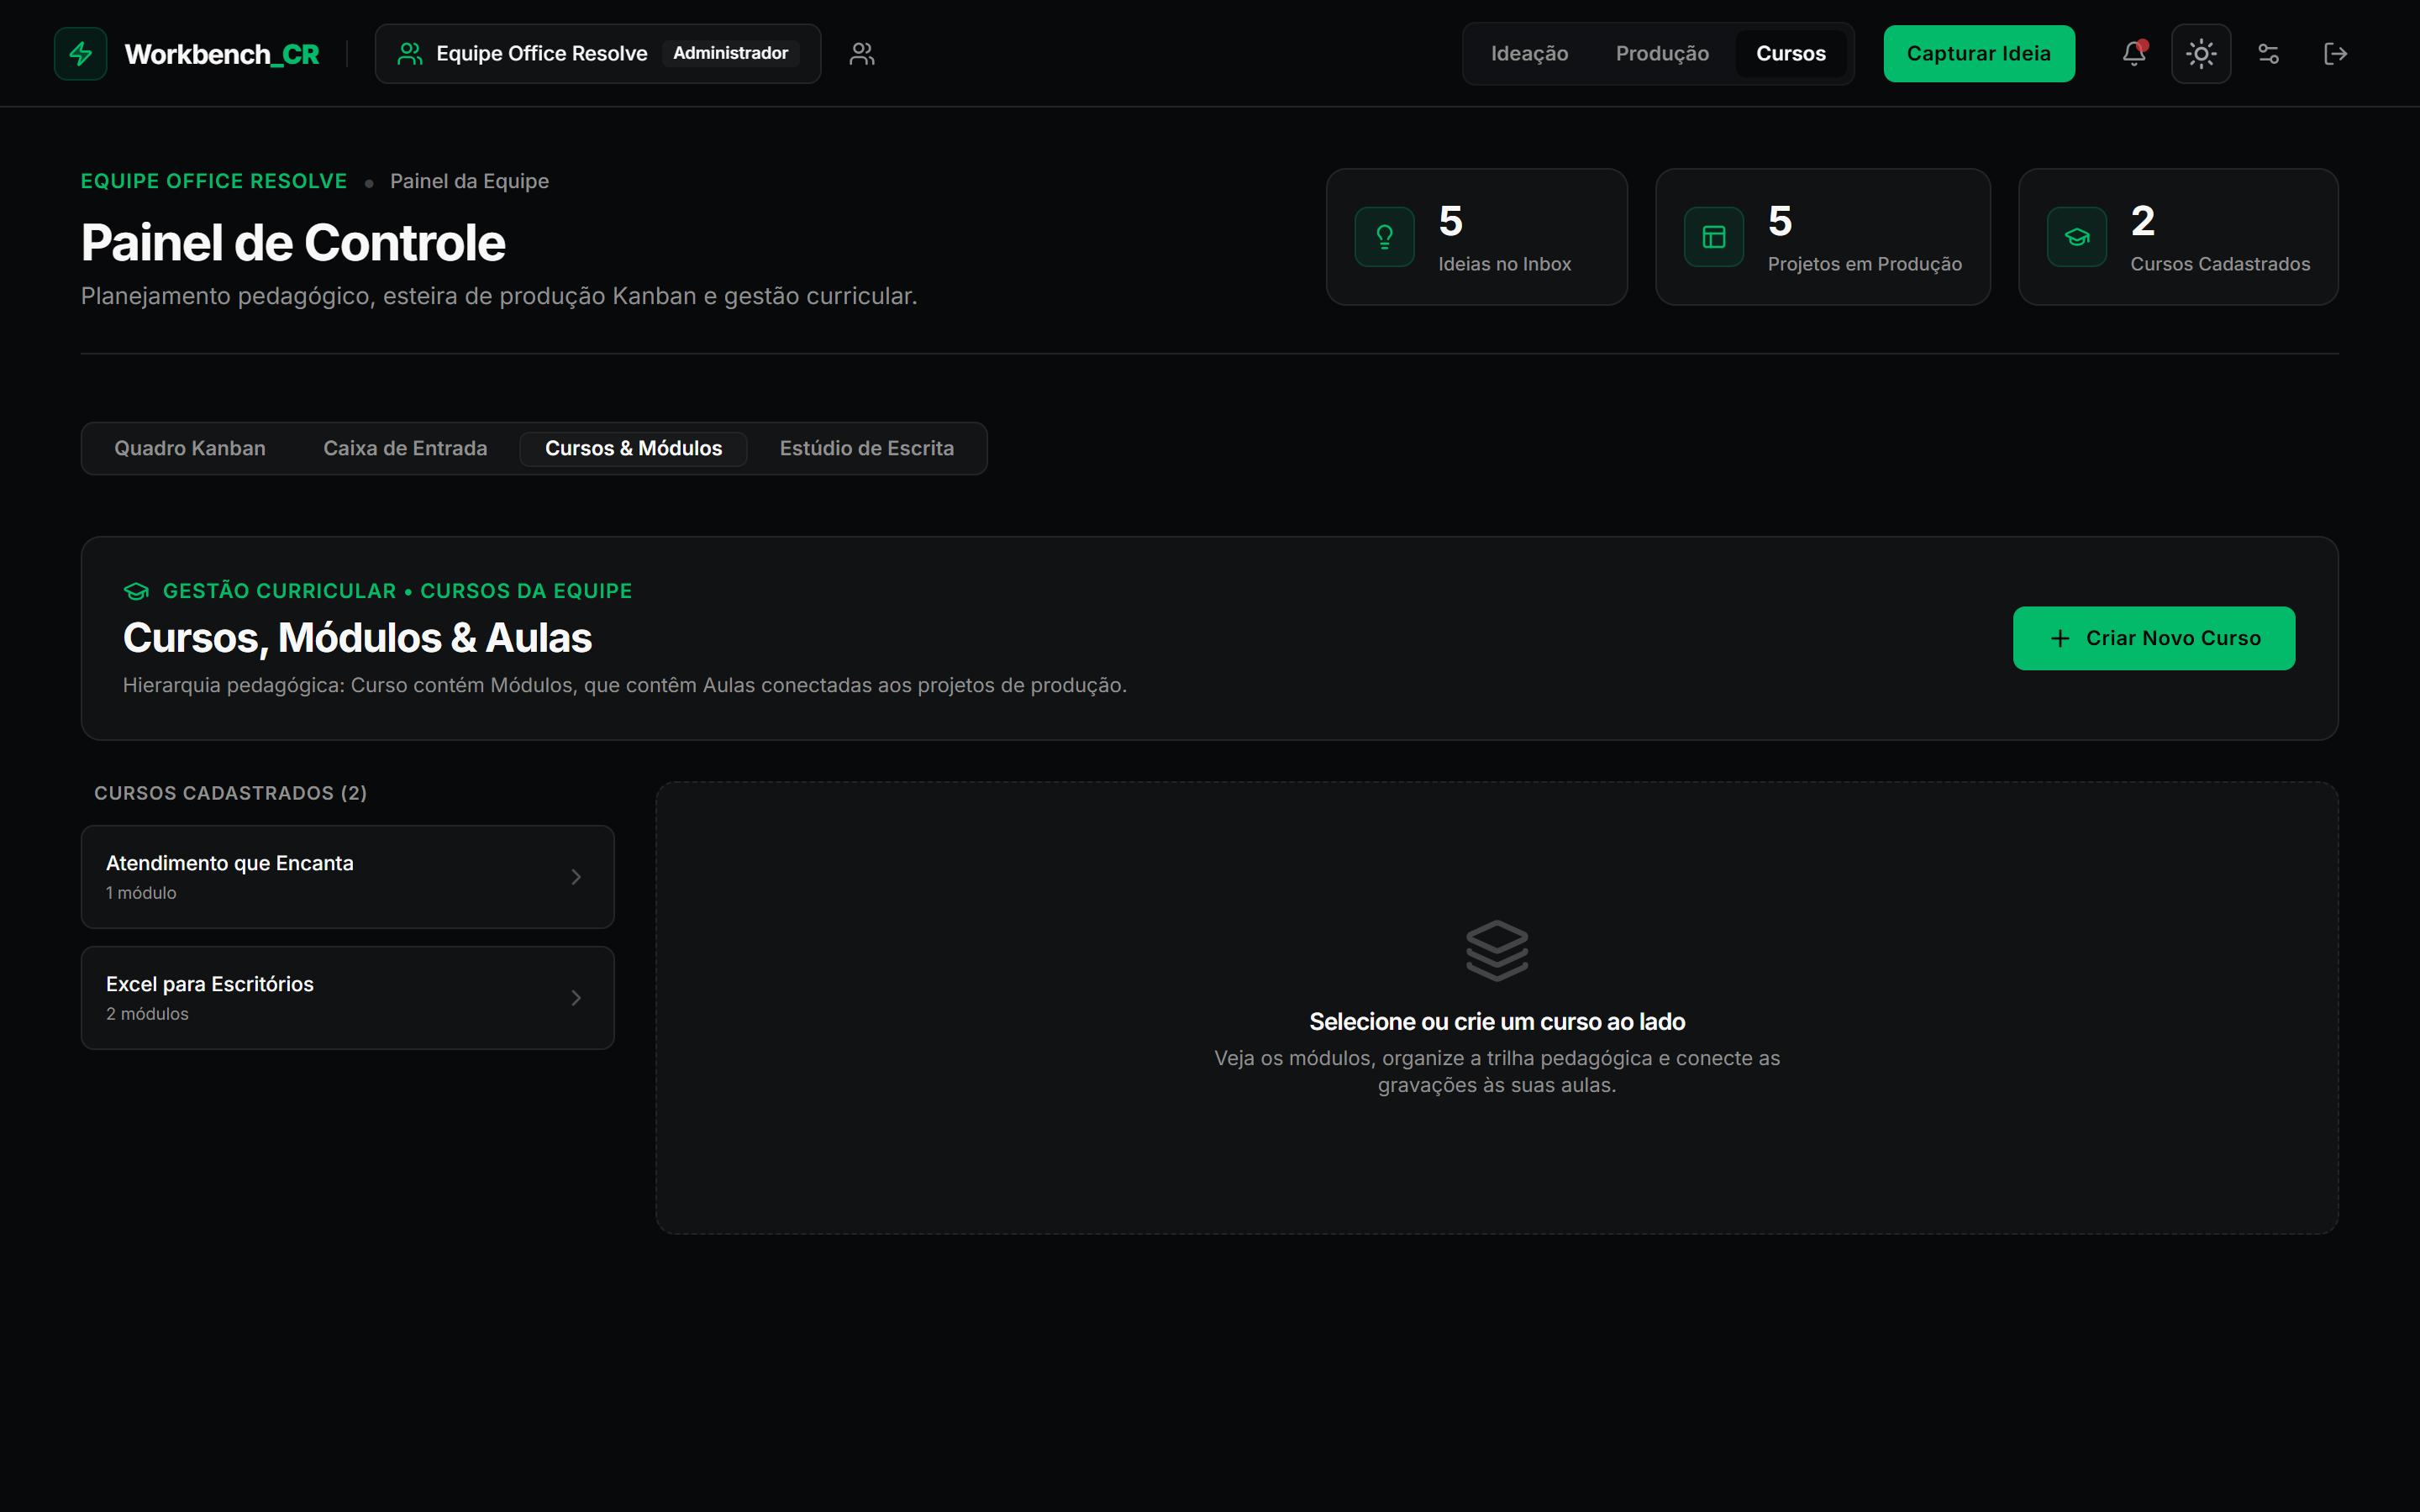
\includegraphics[width=0.85\textwidth]{imagens/17-cursos.png}
    \legend{Fonte: Produzido pelos autores.}
\end{figure}

\begin{figure}[H]
    \centering
    \caption{Curso organizado em módulos e aulas (RF10), com exportação em JSON e CSV (RF11) e botão de publicação}
    \label{fig:tela-18}
    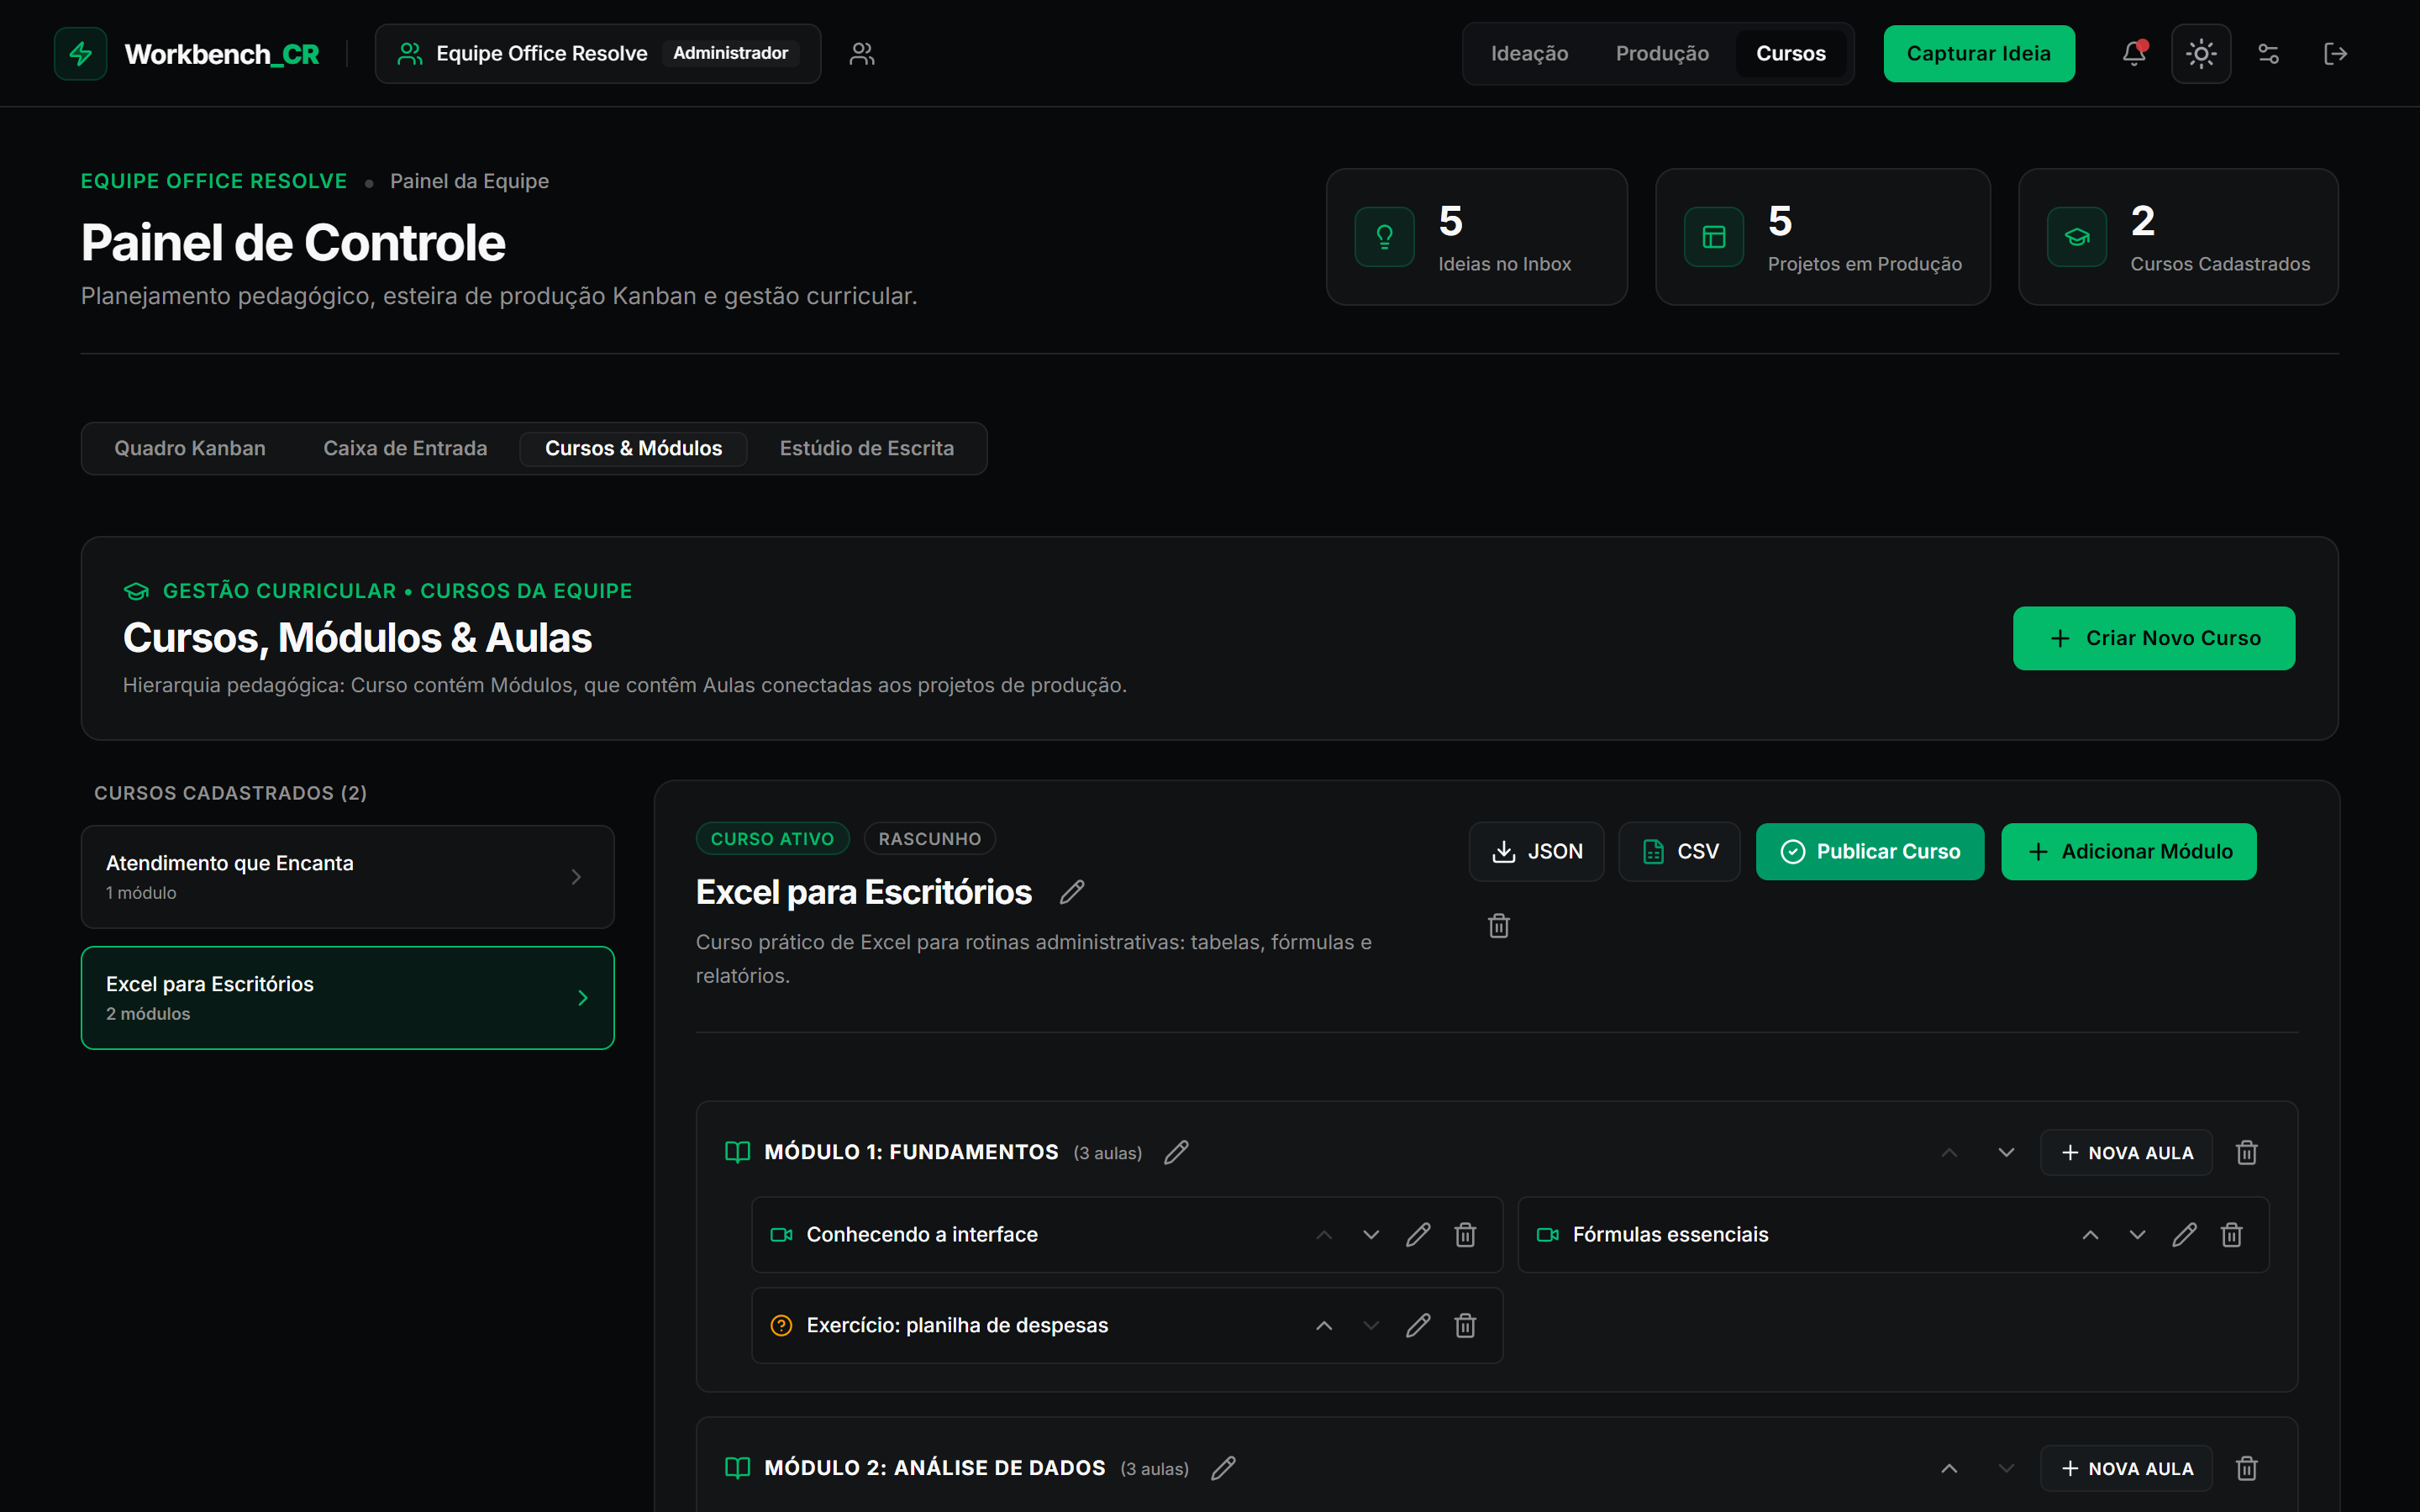
\includegraphics[width=0.85\textwidth]{imagens/18-curso-modulos-e-aulas.png}
    \legend{Fonte: Produzido pelos autores.}
\end{figure}

\begin{figure}[H]
    \centering
    \caption{Confirmação de publicação de um curso que atende às regras de publicação (RN03 e RN06)}
    \label{fig:tela-19}
    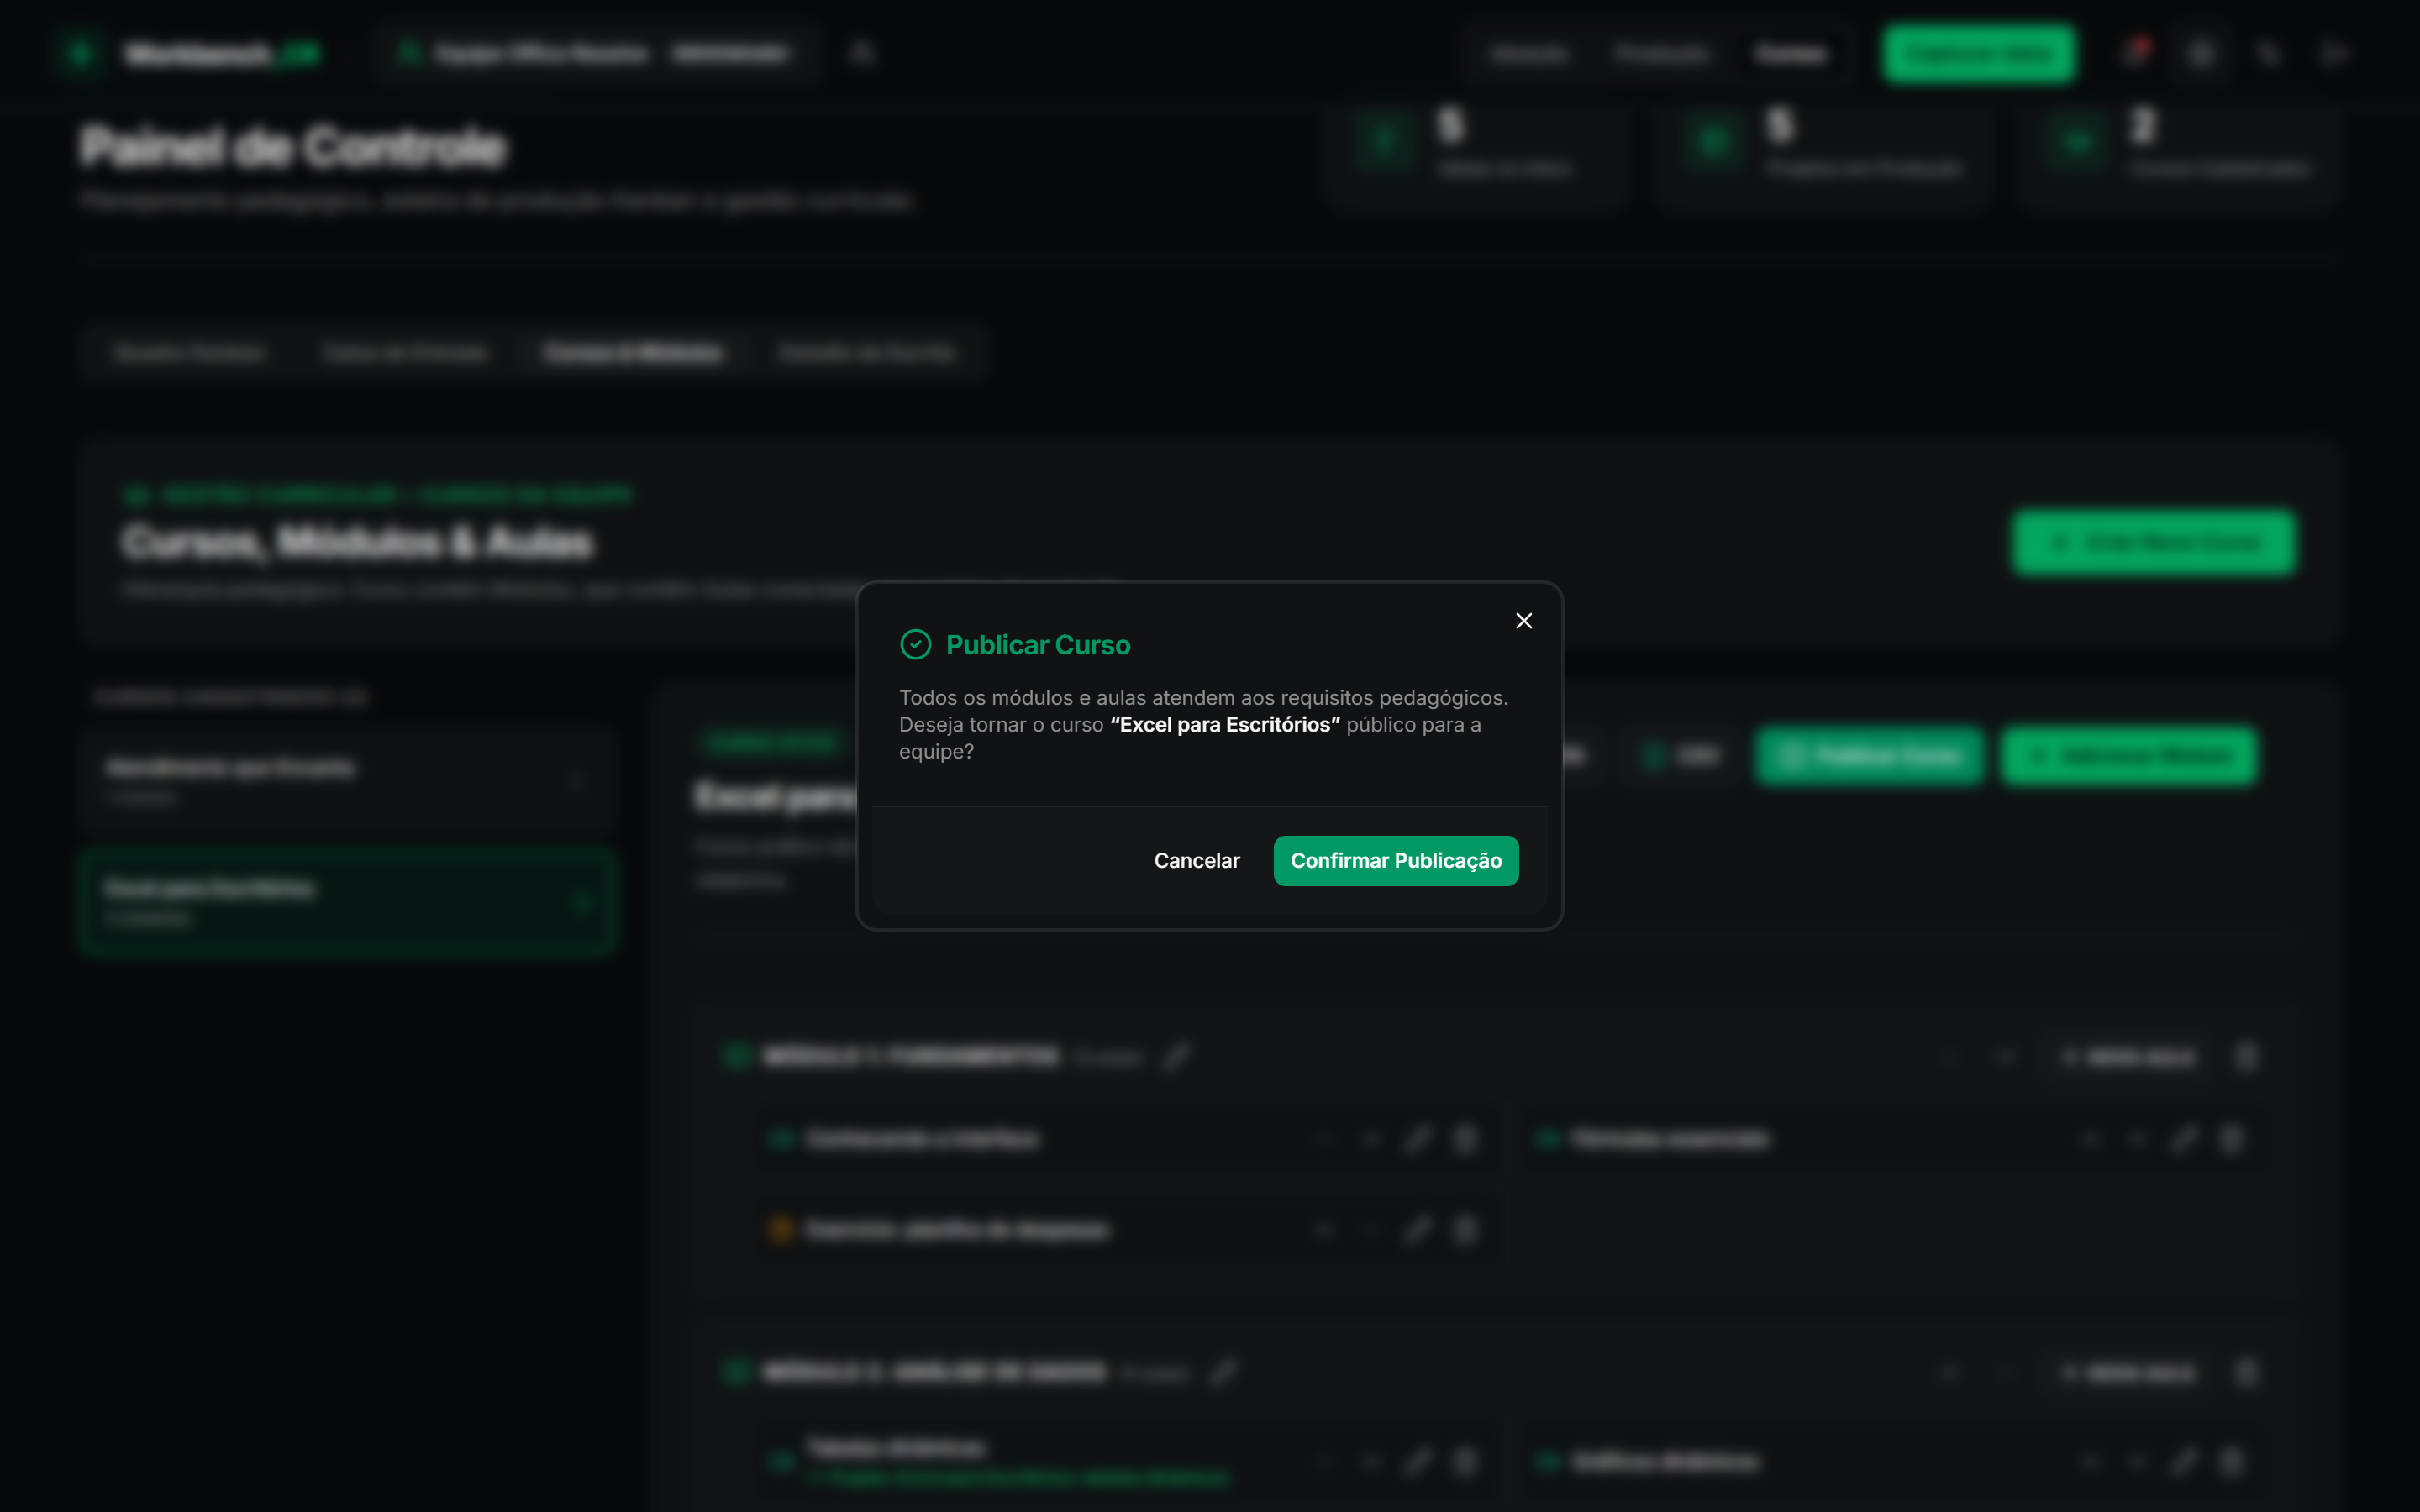
\includegraphics[width=0.85\textwidth]{imagens/19-publicacao-aprovada.png}
    \legend{Fonte: Produzido pelos autores.}
\end{figure}

\begin{figure}[H]
    \centering
    \caption{Publicação bloqueada, com a lista de pendências que o criador precisa corrigir (RN03)}
    \label{fig:tela-20}
    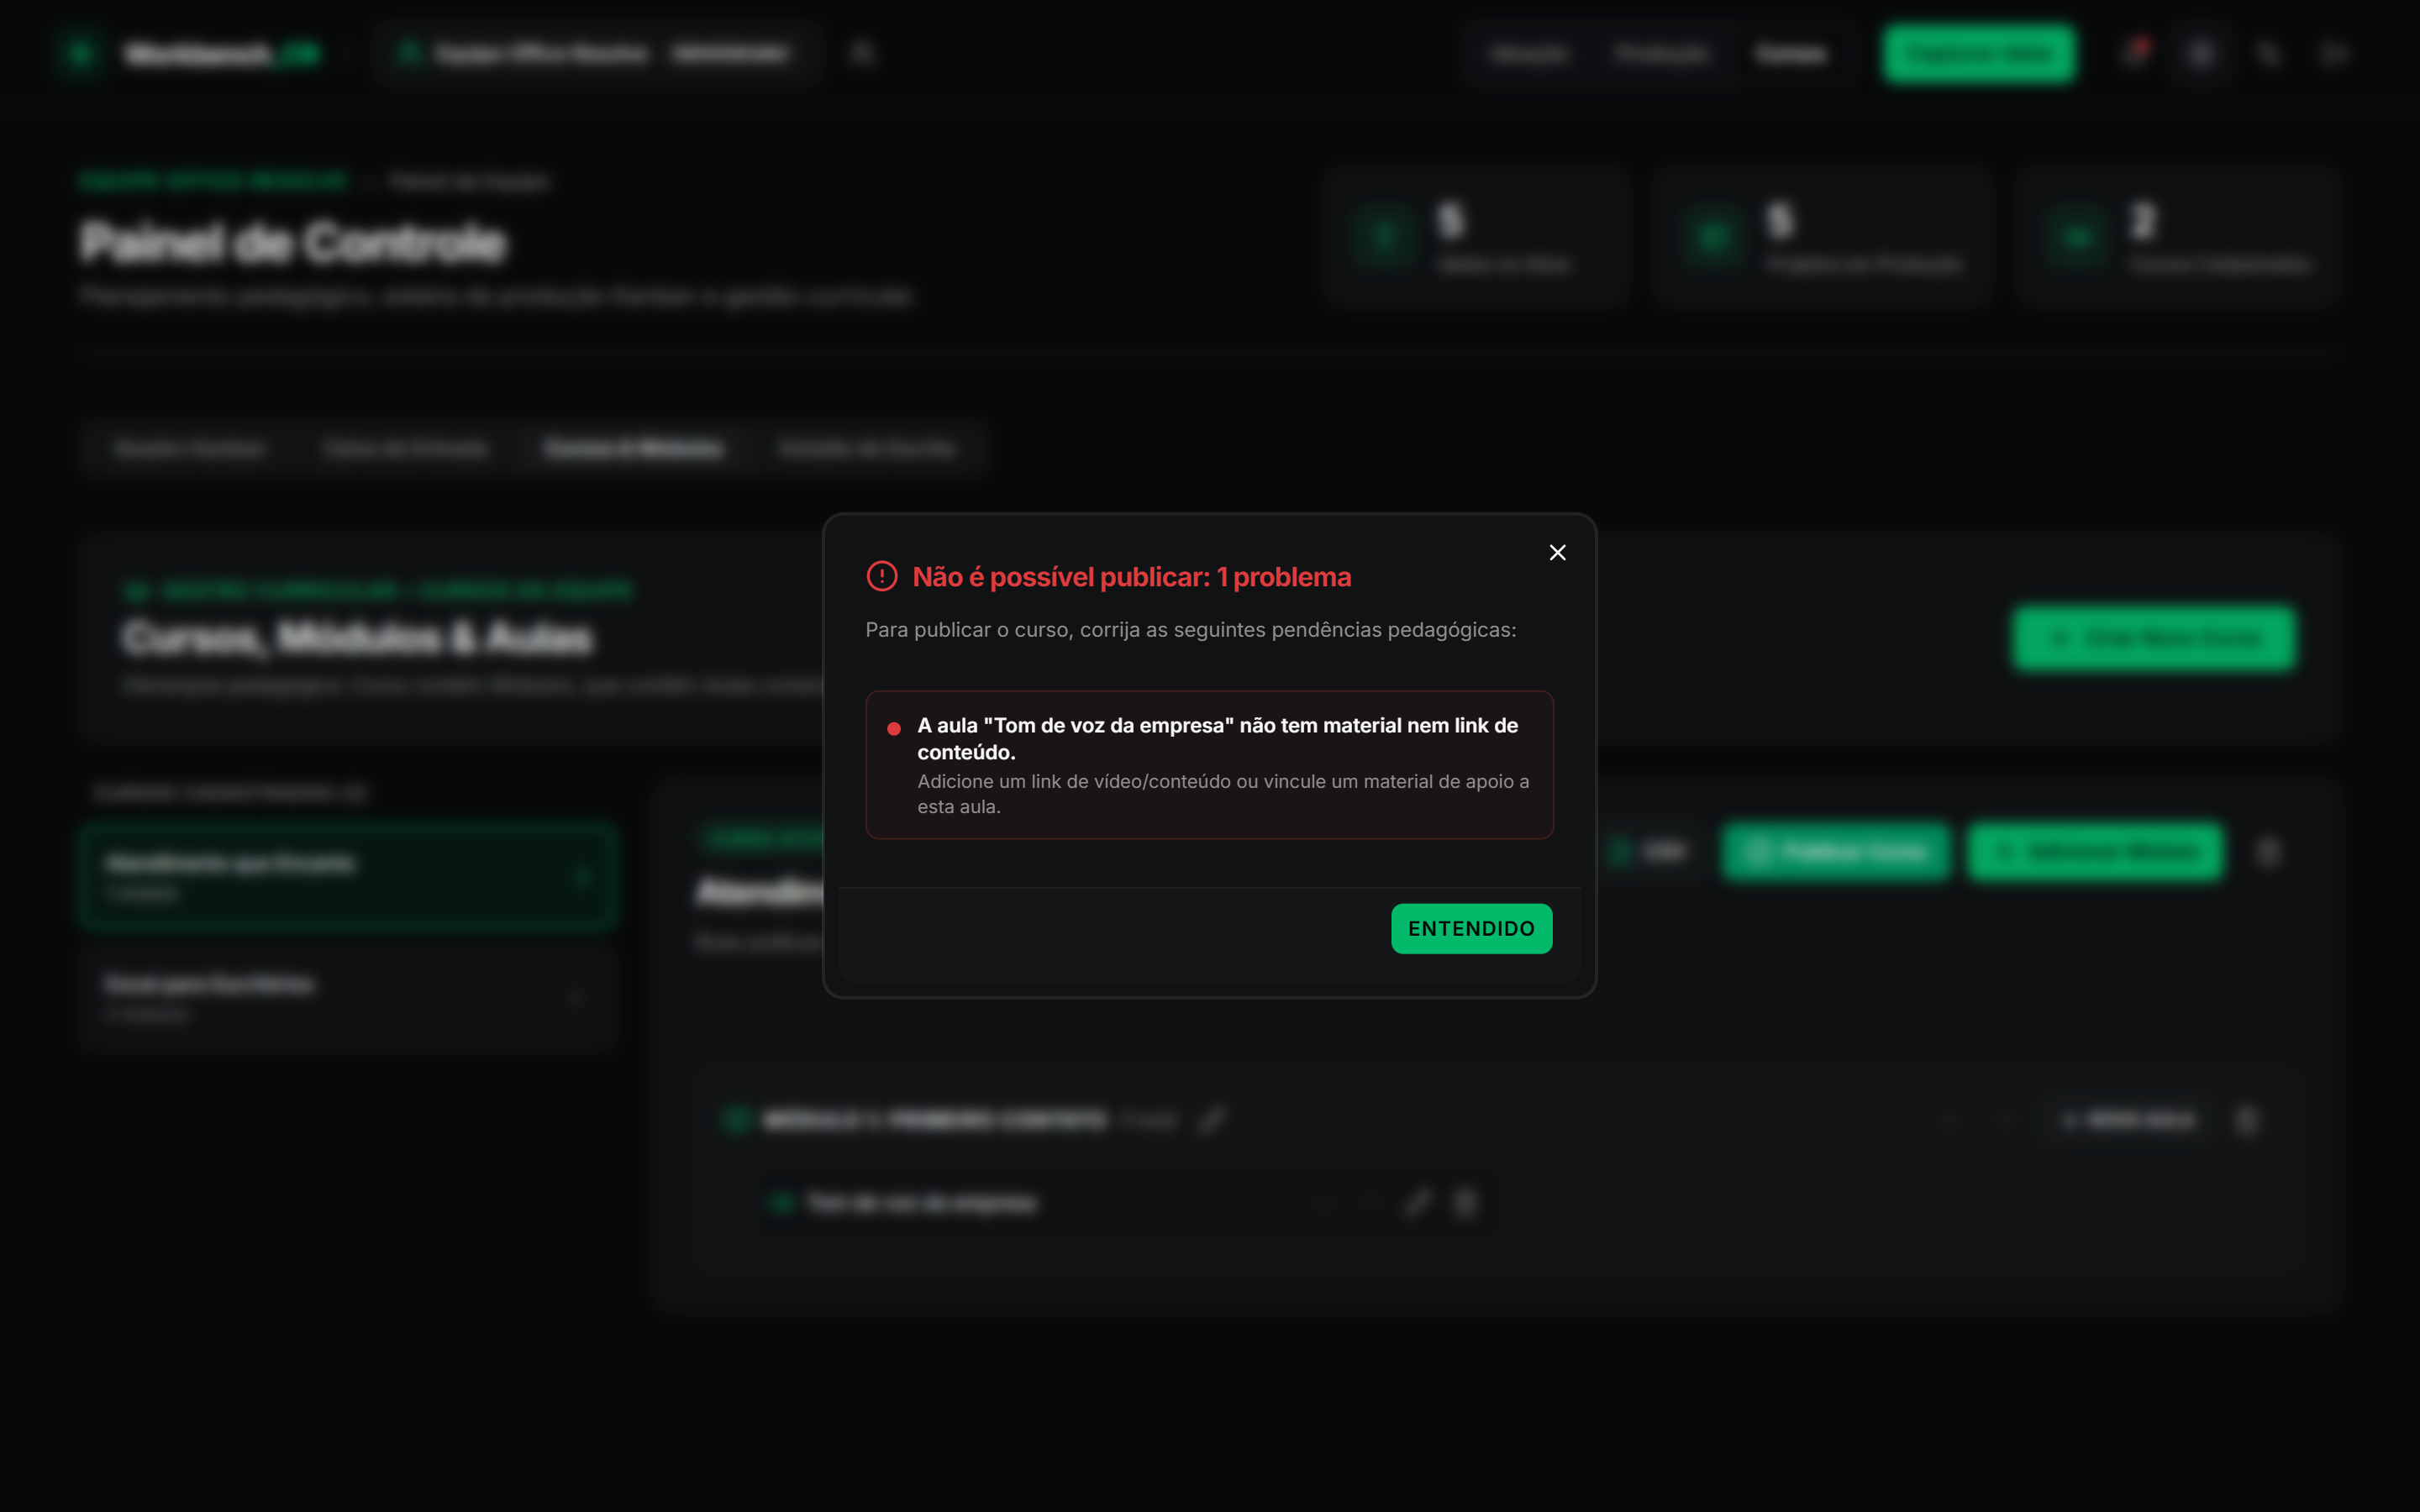
\includegraphics[width=0.85\textwidth]{imagens/20-publicacao-com-pendencias.png}
    \legend{Fonte: Produzido pelos autores.}
\end{figure}

\section{Equipes e conta}

\begin{figure}[H]
    \centering
    \caption{Troca de equipe e criação de nova equipe}
    \label{fig:tela-21}
    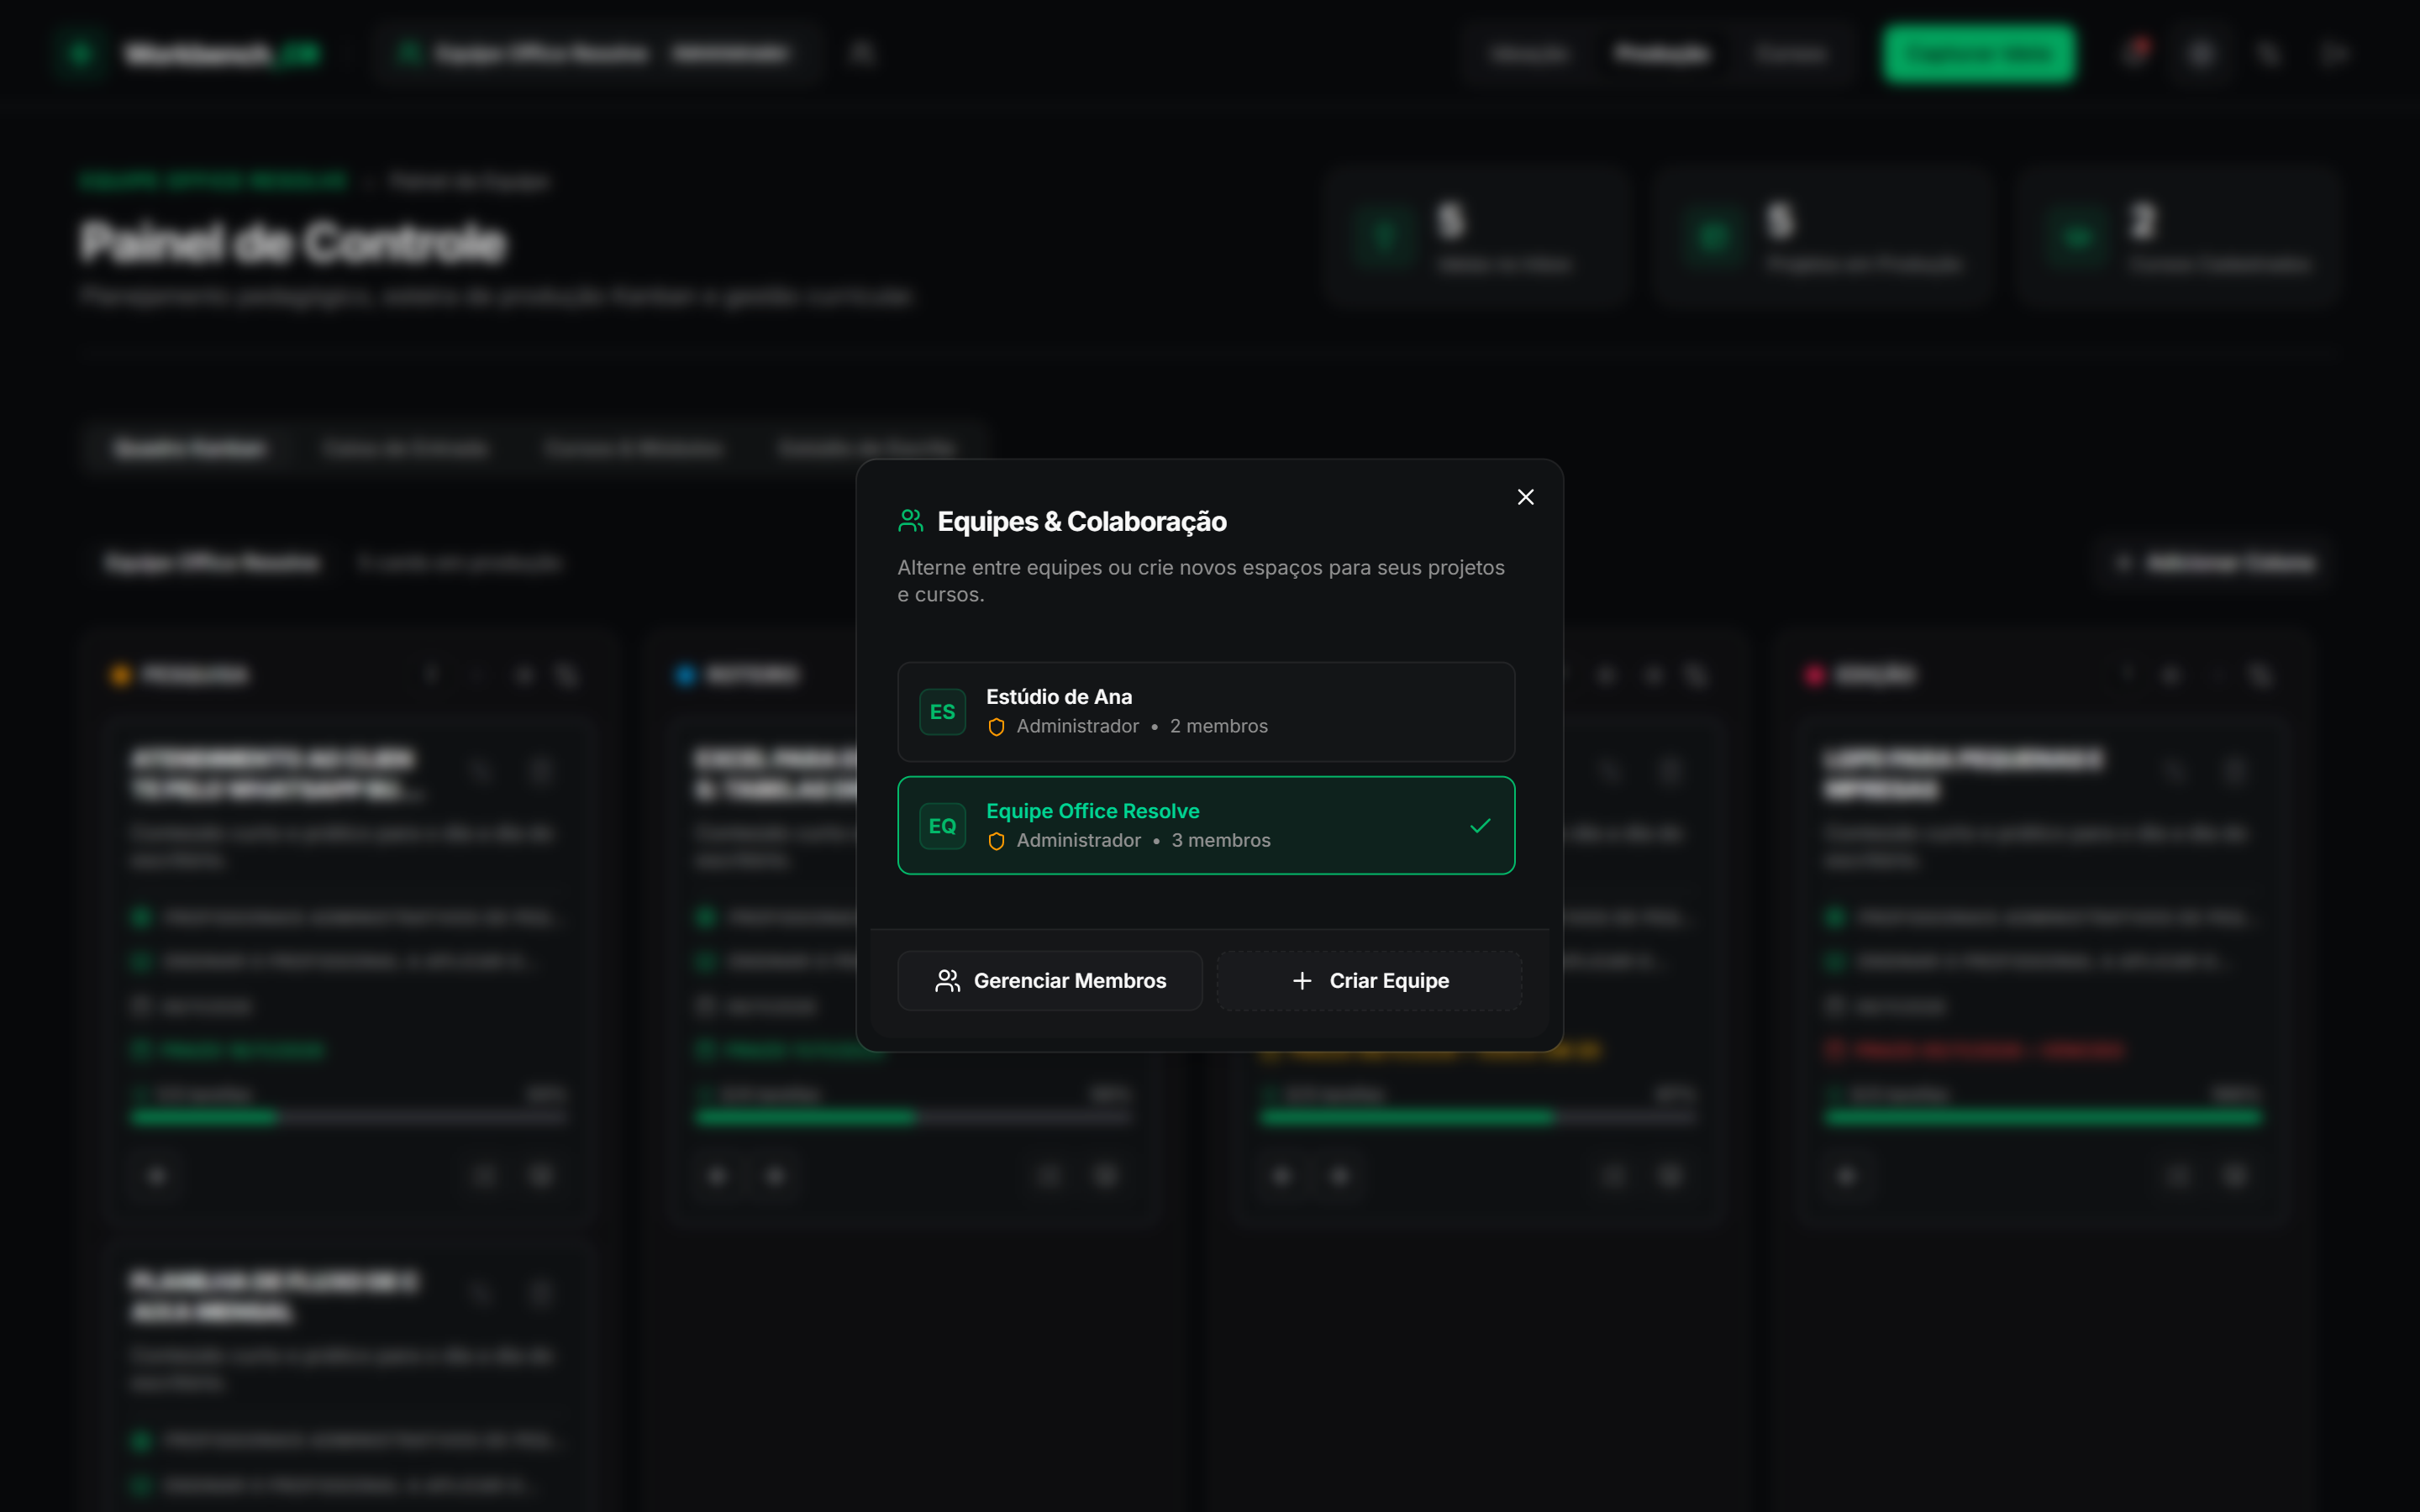
\includegraphics[width=0.85\textwidth]{imagens/21-equipes.png}
    \legend{Fonte: Produzido pelos autores.}
\end{figure}

\begin{figure}[H]
    \centering
    \caption{Gestão dos membros da equipe e de seus papéis: Administrador, Criador e Revisor (RF02)}
    \label{fig:tela-22}
    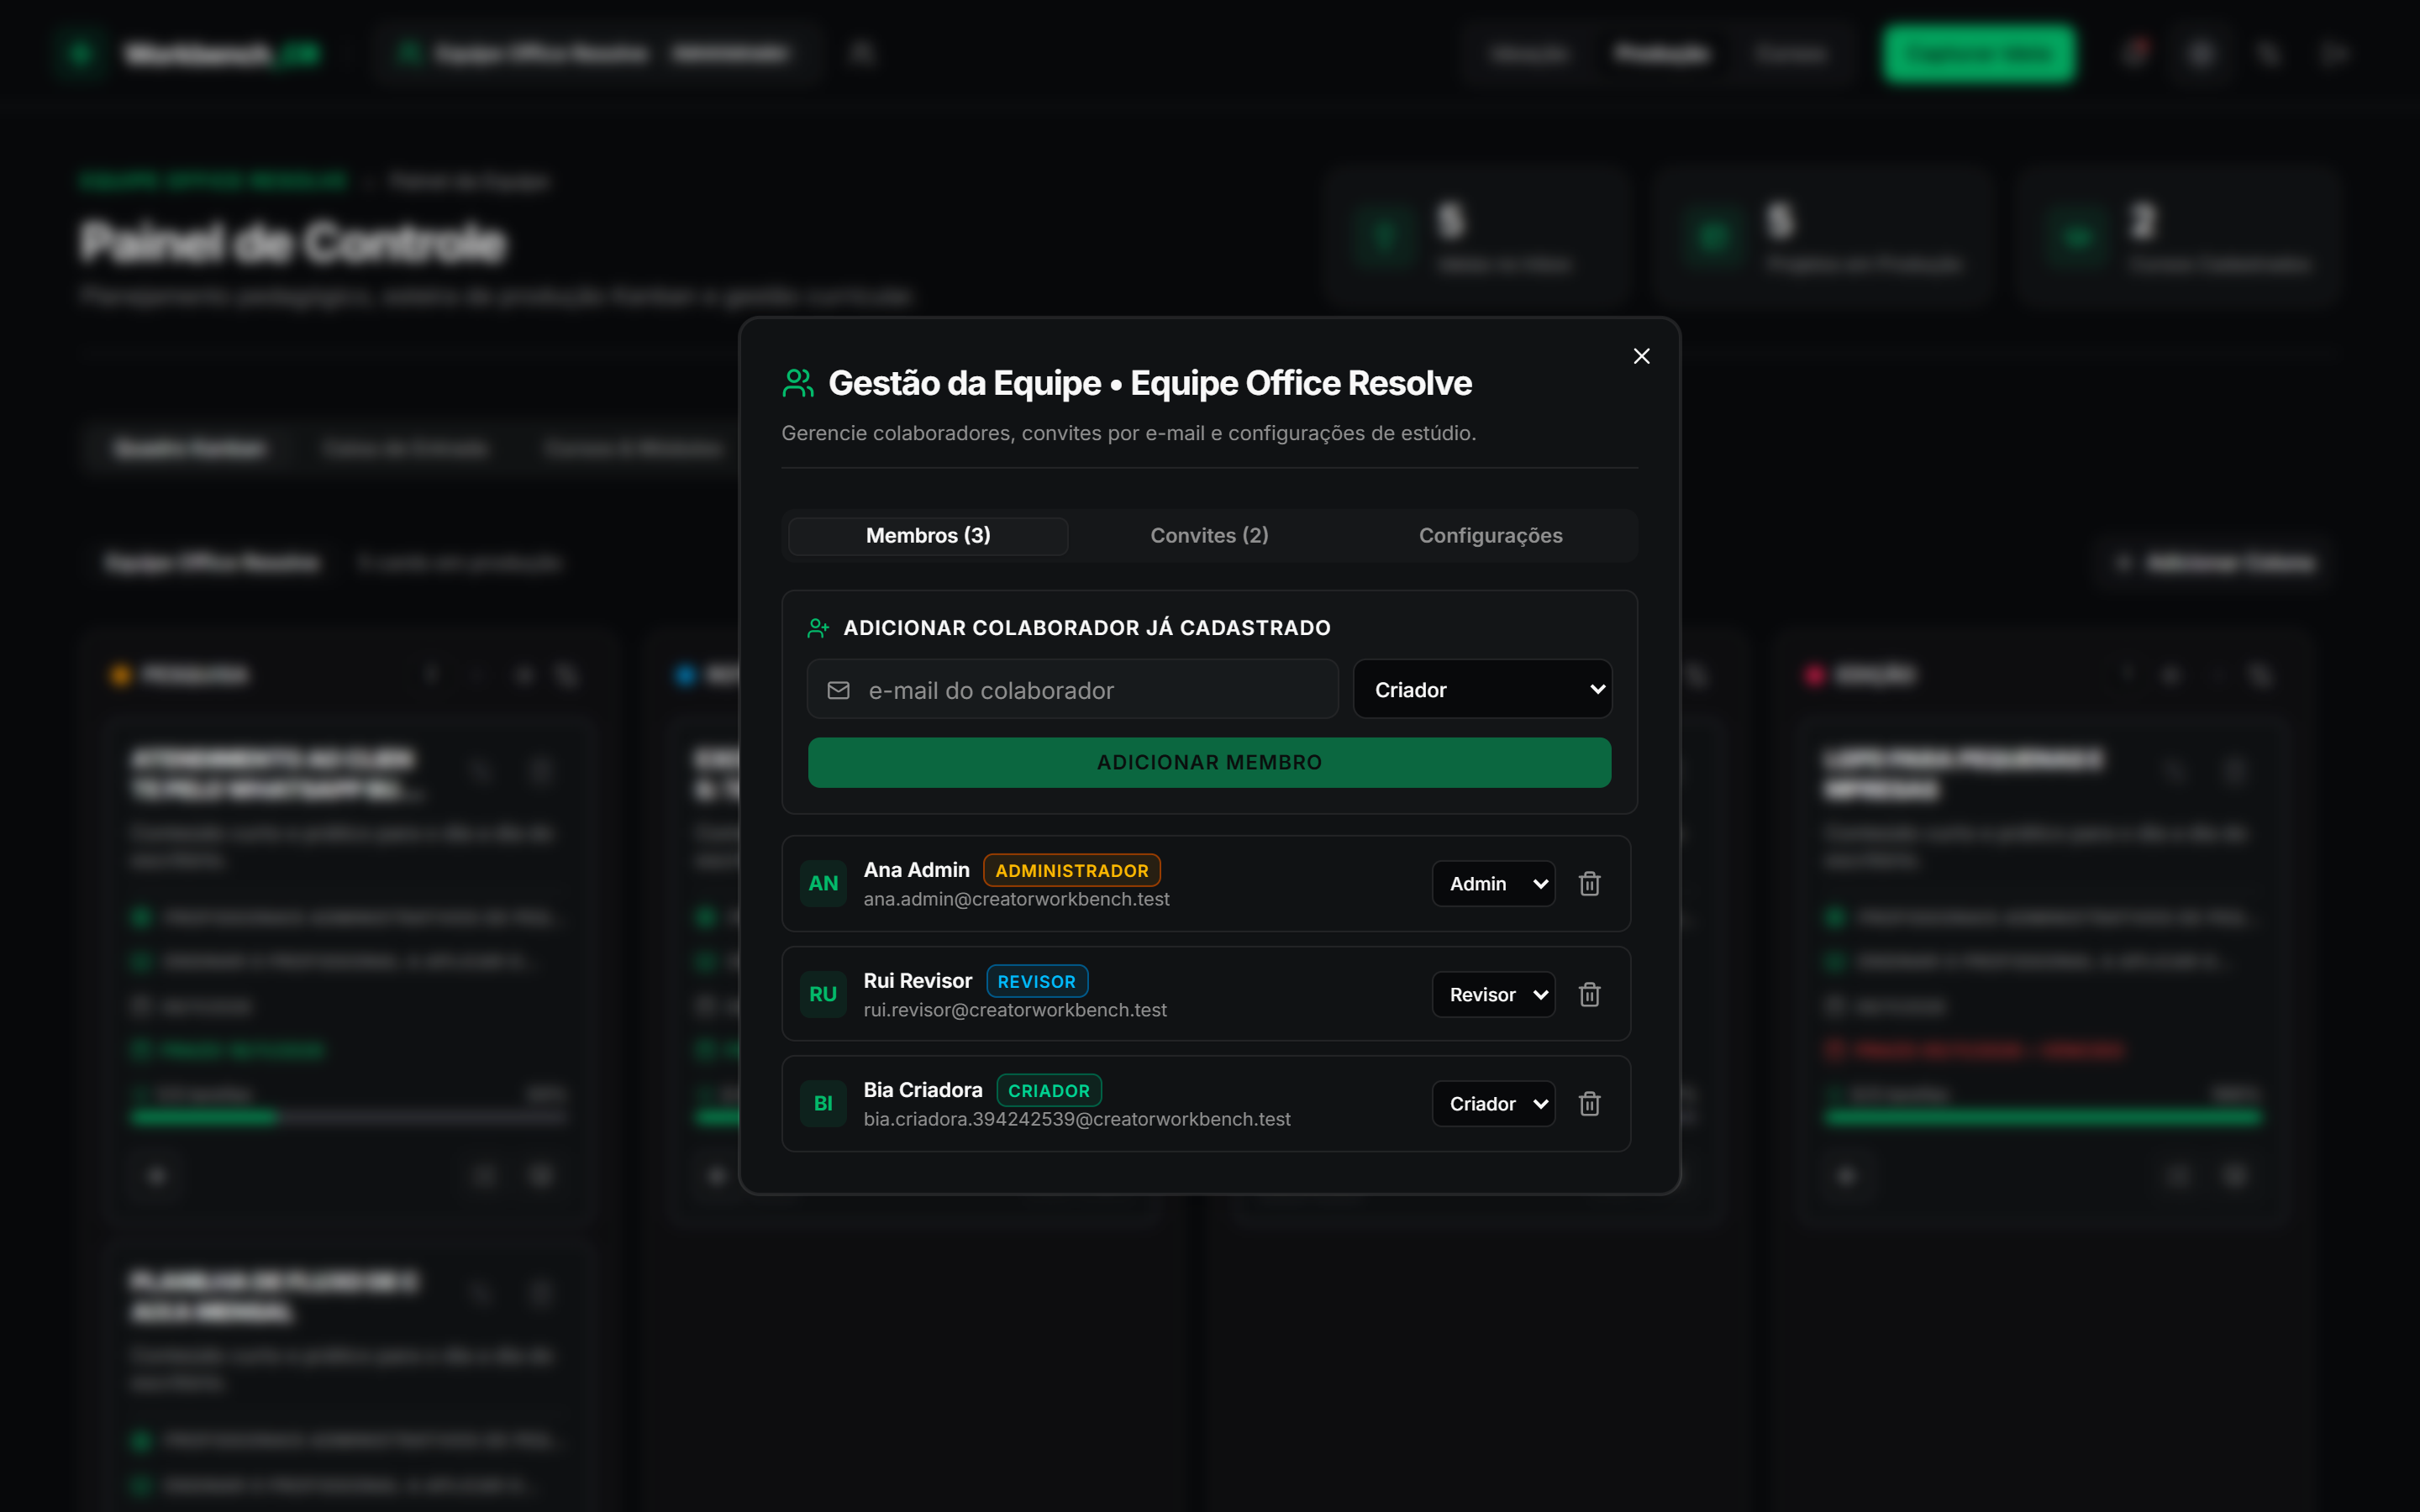
\includegraphics[width=0.85\textwidth]{imagens/22-membros-da-equipe.png}
    \legend{Fonte: Produzido pelos autores.}
\end{figure}

\begin{figure}[H]
    \centering
    \caption{Convites por e-mail, válidos por 7 dias, com o papel de cada convidado}
    \label{fig:tela-23}
    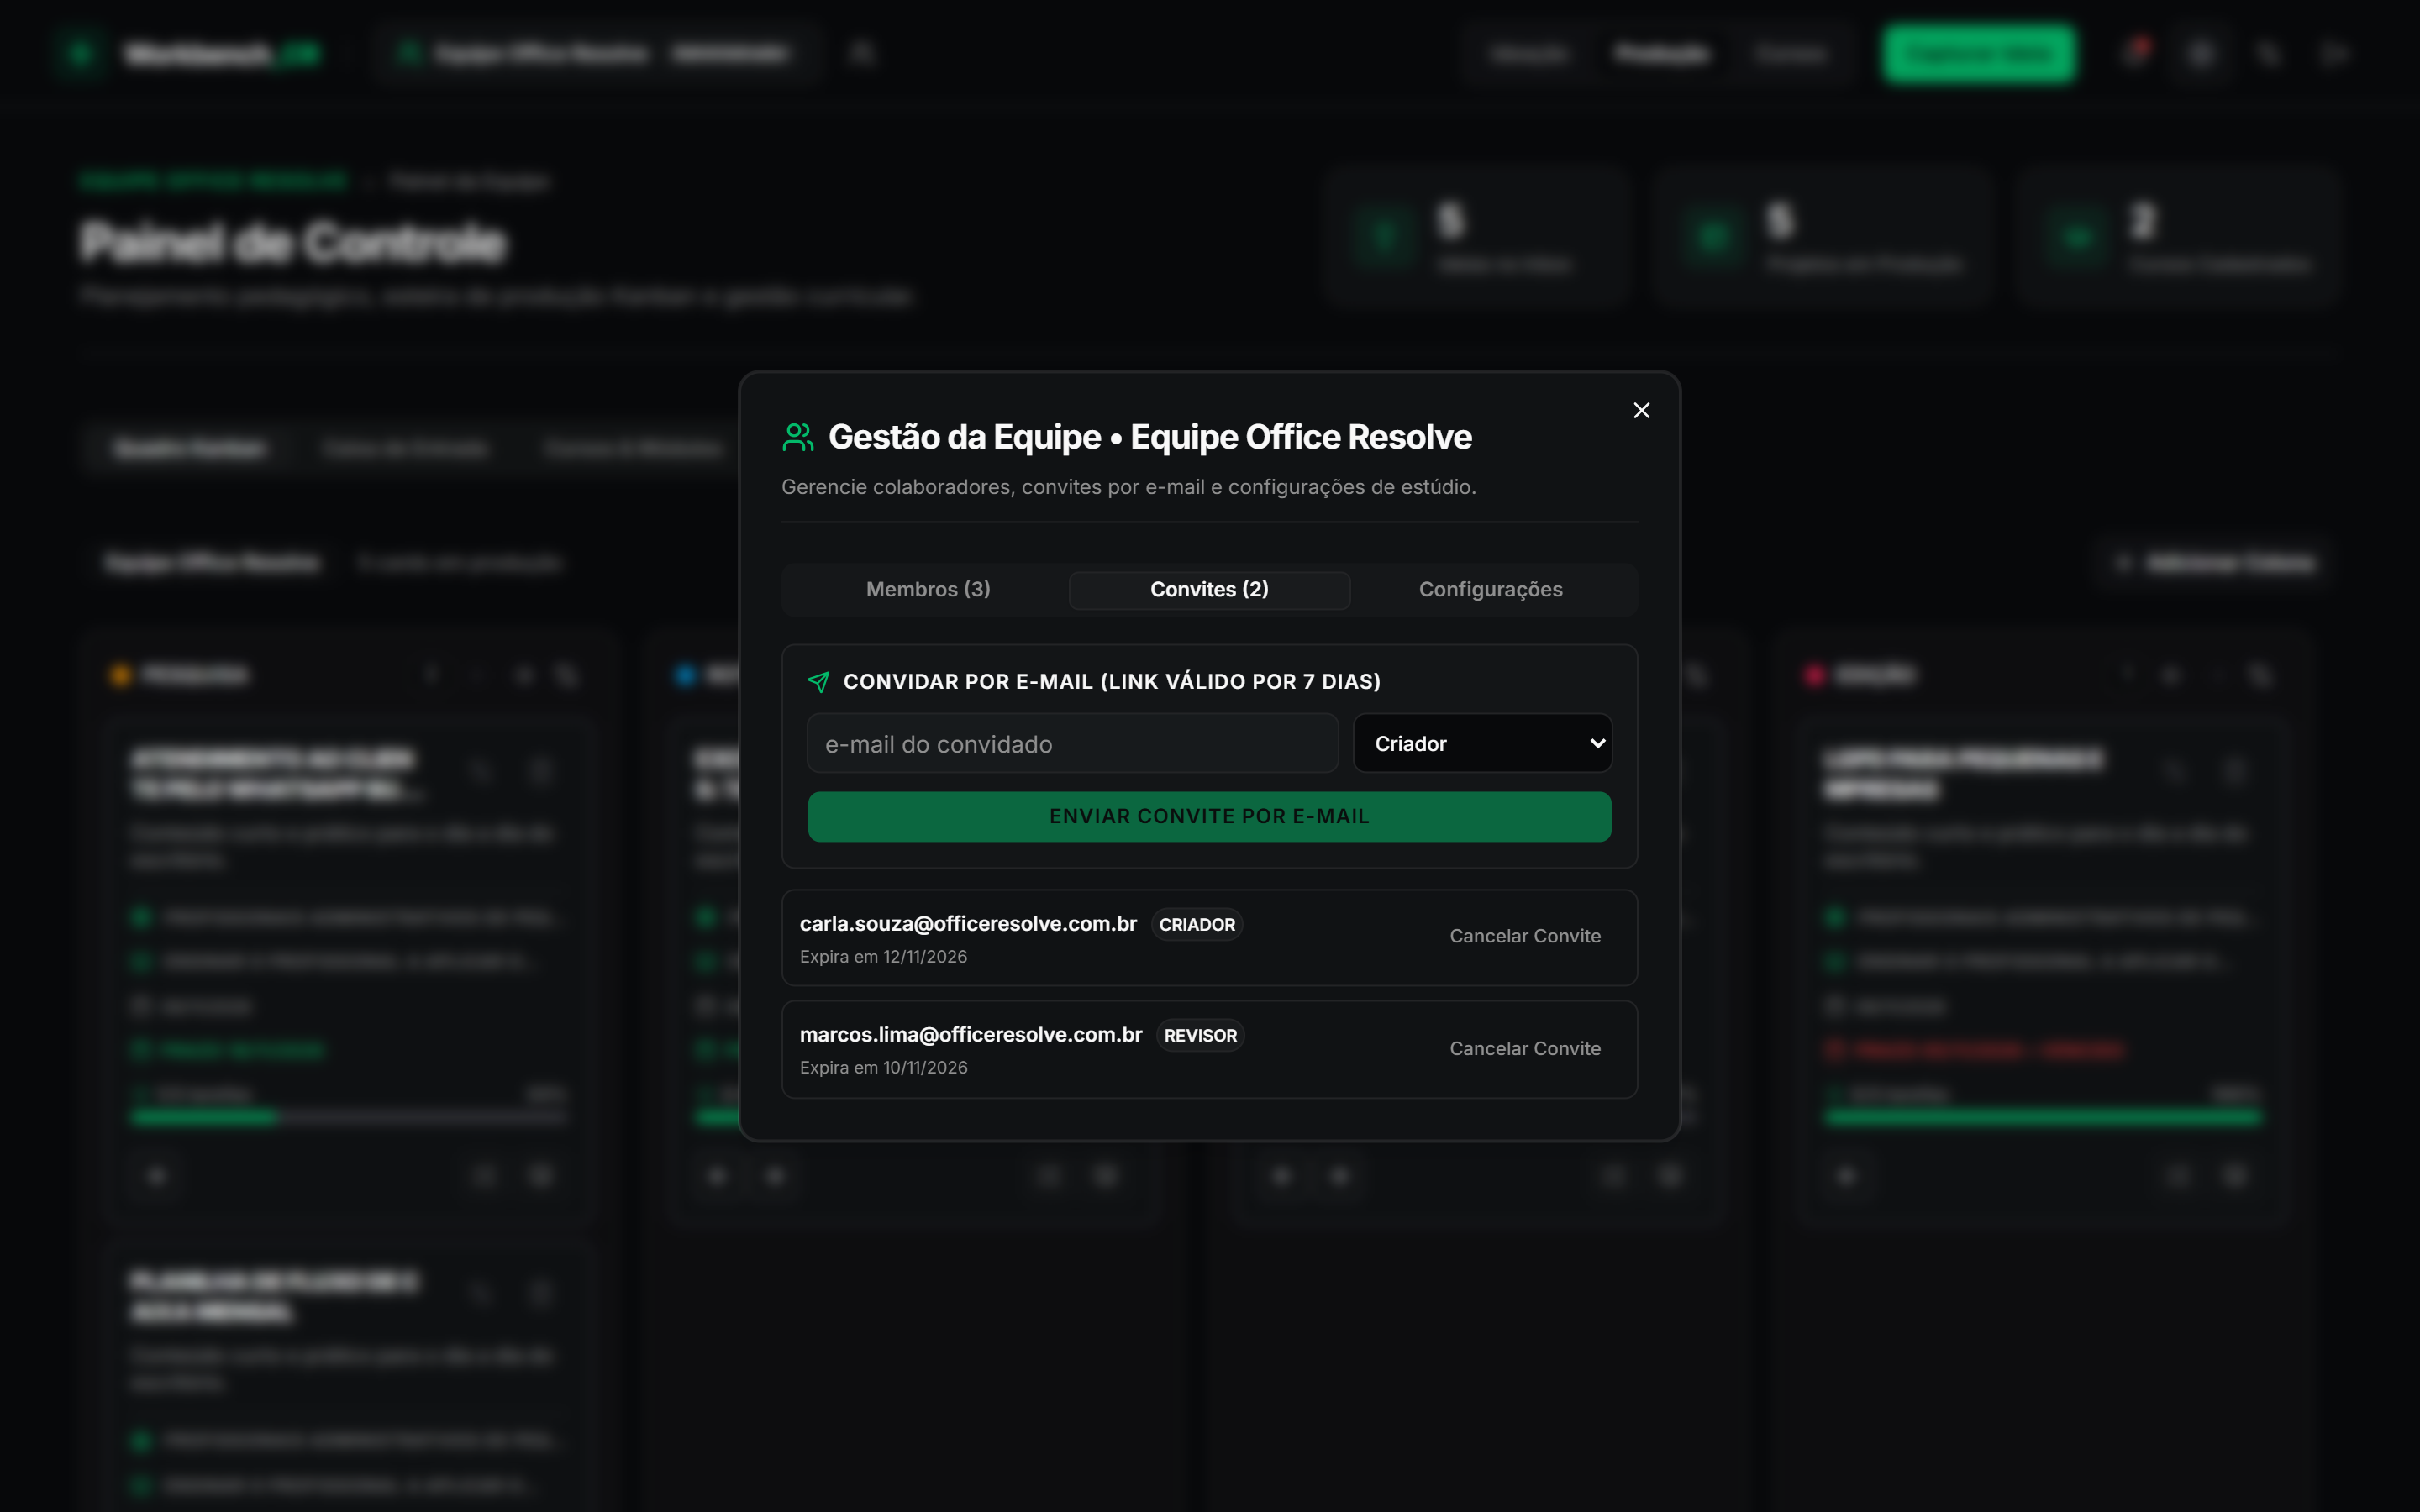
\includegraphics[width=0.85\textwidth]{imagens/23-convites-da-equipe.png}
    \legend{Fonte: Produzido pelos autores.}
\end{figure}

\begin{figure}[H]
    \centering
    \caption{Configurações da conta, com nome, e-mail, senha e exclusão da conta}
    \label{fig:tela-24}
    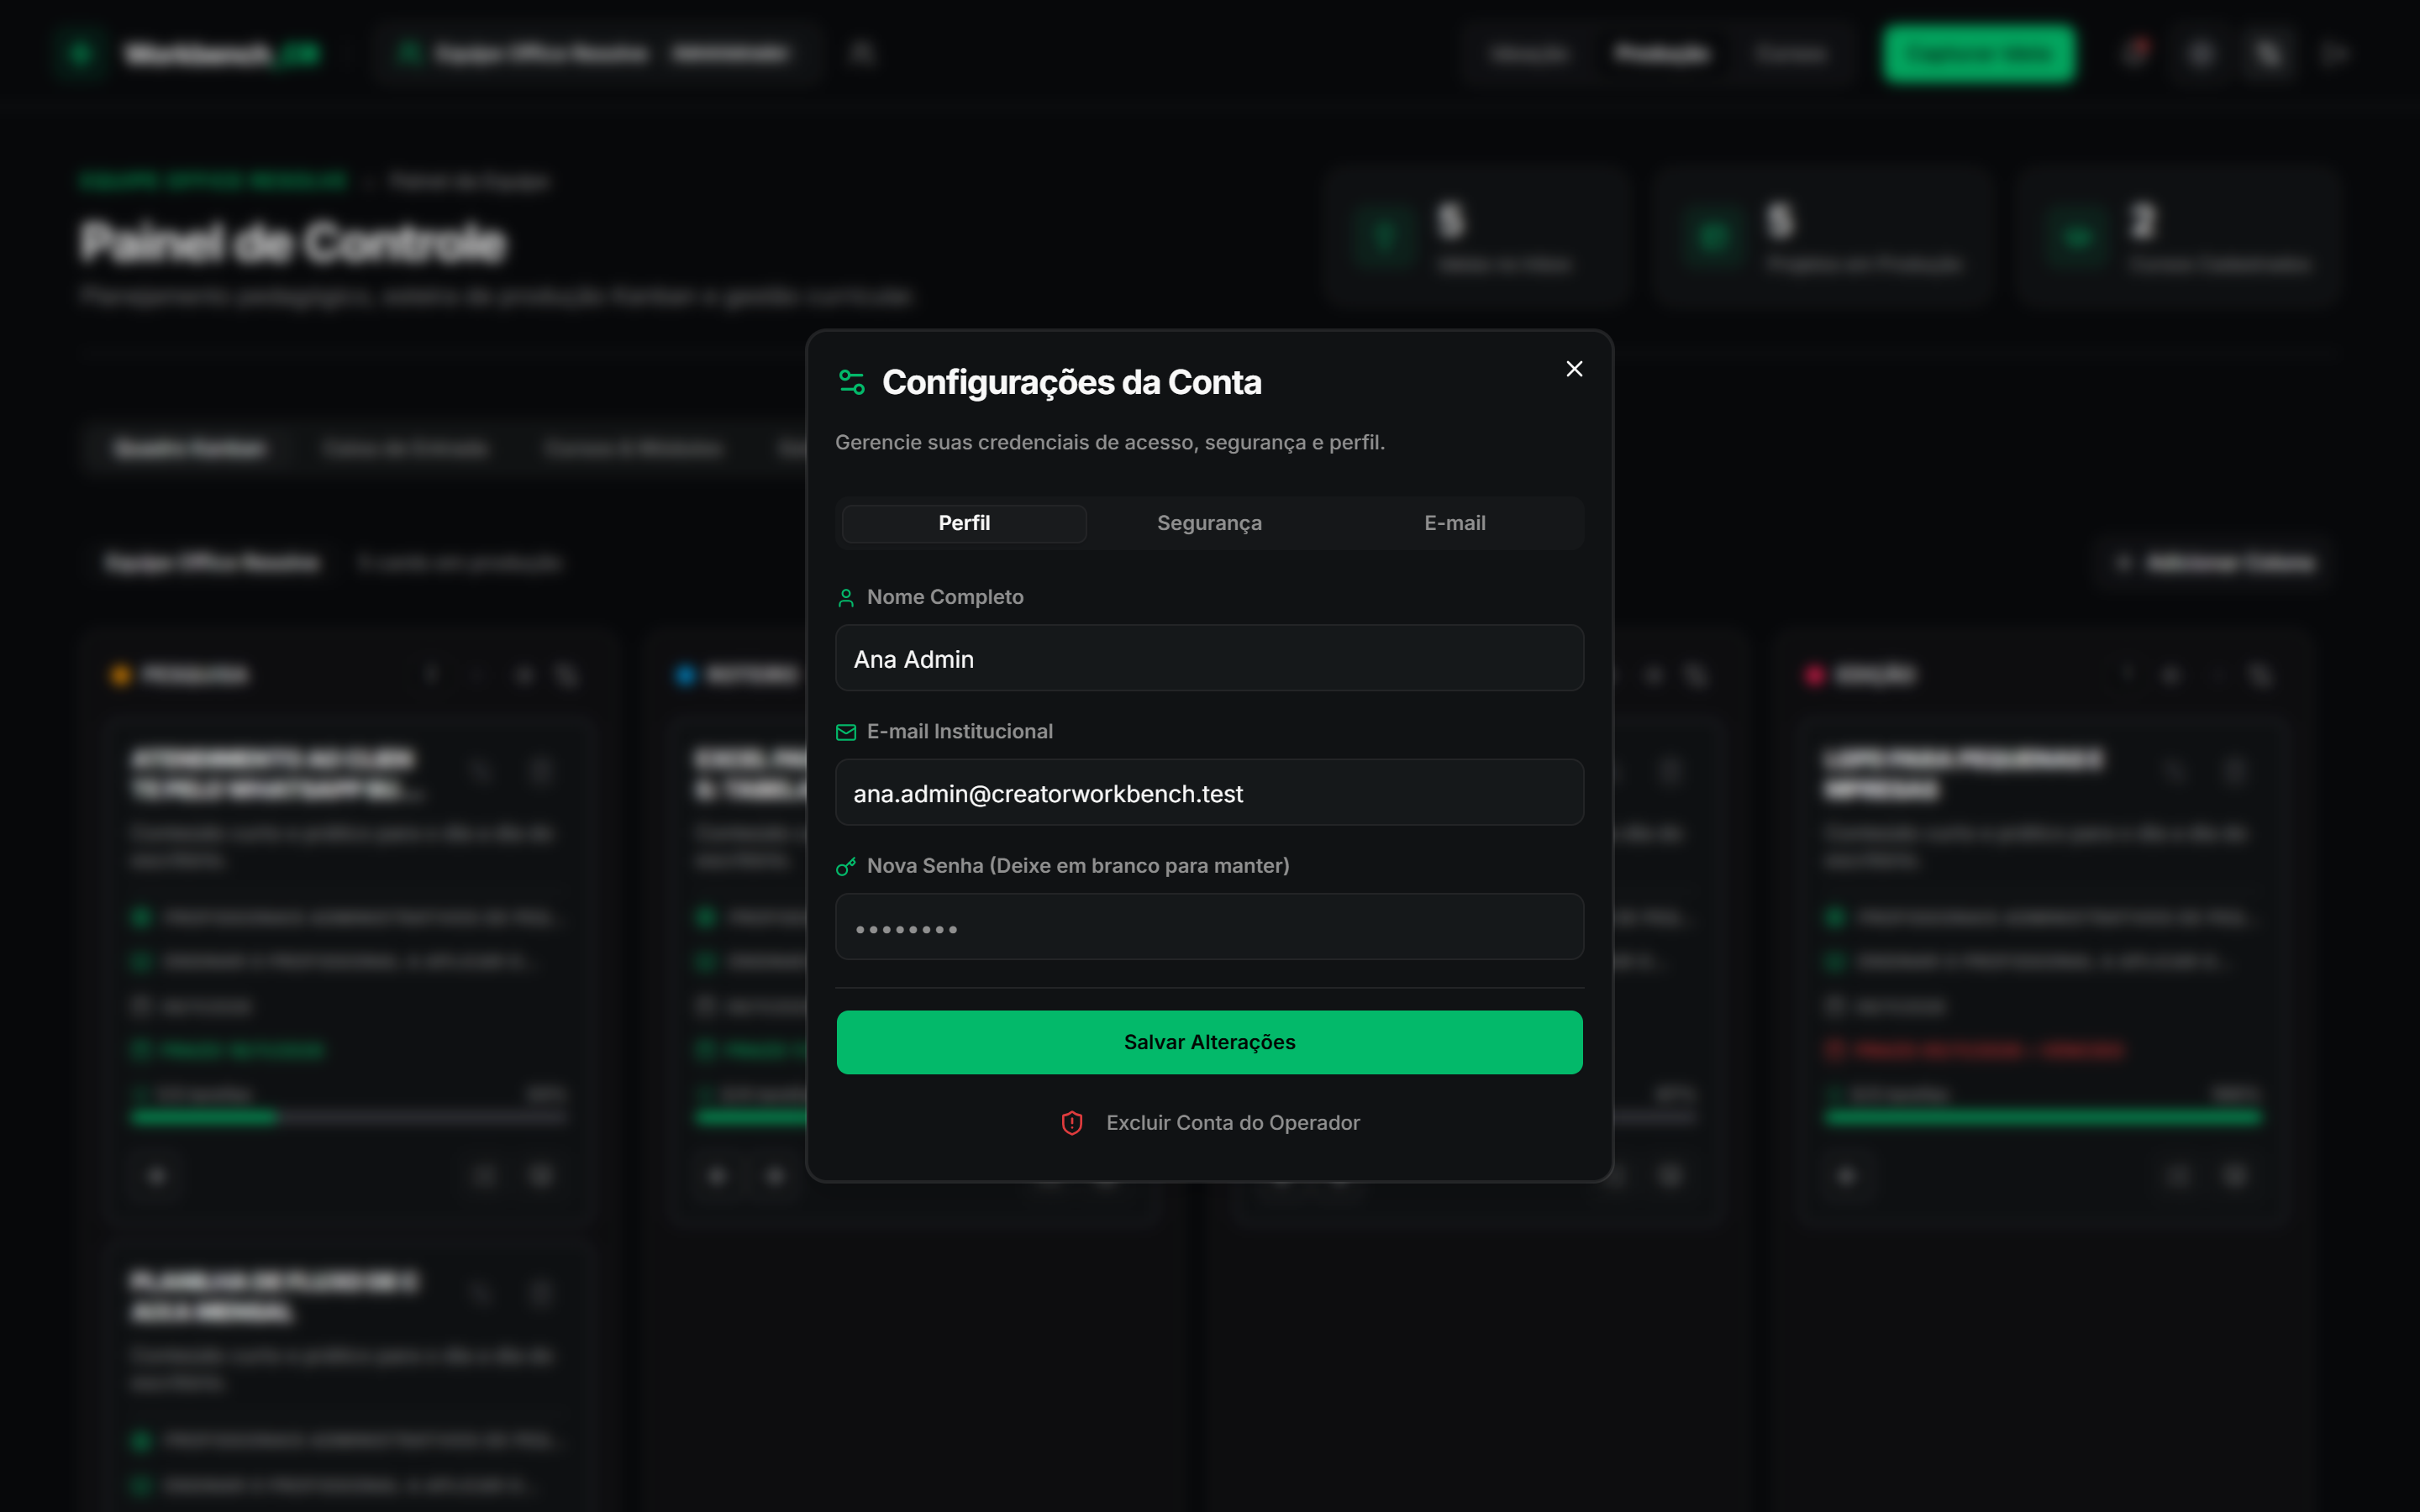
\includegraphics[width=0.85\textwidth]{imagens/24-configuracoes-do-usuario.png}
    \legend{Fonte: Produzido pelos autores.}
\end{figure}

\end{apendicesenv}
